\chapter[Application of models to HSI data]{Application of analytical tissue models to Hyperspectral Imaging data}\label{chap:HSImodel}
\begin{center}
\begin{minipage}[b]{0.9\linewidth}
\small
\textbf{Foreword\,}
This chapter is as yet unpublished. 
\newline
AB has conducted all of the research presented in this chapter under the supervision of JS, MB, and TV. The gelatin-based phantom images were annotated by OM. 
\end{minipage}
\end{center}

\minitoc

\section{Introduction}
As described in Chapter \ref{chap:intro}, hyperspectral imaging (HSI) is able to capture spatially resolved, diffuse reflectance spectra via non-contact imaging~\citep{Lu2014,Giannoni2018,Calin2014,Shapey2019}, which could enable quantitative, spatially-resolved, tissue oxygenation ($StO_2$) extraction. Many methods have been considered for this ranging from two or three wavelength approaches~\citep{Clancy2020} to wavelength-dependent analytical models including those investigated in Chapters \ref{chap:1layer} and \ref{chap:2layer} as these have been some of the prominent methods of doing so~\citep{Yudovsky2009, Jacques1999, Clancy2015, Clancy2020}. Other methods include deep-learning based approaches, however these rely on models or simulation to generate their training data~\citep{Wirkert2016}, or models based on the derivatives of the spectra, however these rely on extensive calibration and assume that the scattering contribution is wavelength-independent which may not be true for all tissues~\citep{Holmer2018}.

HSI data is often of lower spectral resolution than the spectrophotometer data tested in the previous chapters, particularly that of snapshot HSI data which compromises spectral resolution in favour of shorter aquisition times~\citep{Geelen2014}. Additionally, hyperspectral imaging is known to suffer from spectral noise which may be reduced significantly by spatial averaging~\citep{Zhang2020}.

In this chapter, we quantify the impact of reducing the spectral resolution and introduction of noise on the performance of the analytical models investigated in Chapters \ref{chap:1layer} and \ref{chap:2layer} by simulating a snapshot camera response from the Monte Carlo datasets used in these previous chapters. These impacts are then evaluated with experimental HSI data of the phantoms detailed in Chapter \ref{chap:1layer}. Finally, the models are applied to neurosurgical HSI data obtained intra-operatively as part of the HELICoiD dataset~\cite{Fabelo2019}. % and NHSI datasets. 

\section{Methods}
\subsection{Camera response simulation}\label{sec:MCcameras}
To obtain datasets of simulated data with known ground truth parameters, the datasets described in Sections \ref{sec:methodsMC} and \ref{sec:methodreference2} of internal and skin tissues are used. For each spectrum in the dataset, the camera response is simulated by convolving the band responses of the snapshot HSI camera (depicted in Figures \ref{fig:rulerspectrum} and \ref{fig:simulatingcam}) and the integral of this is divided by the band response integral as defined in Equation \eqref{eq:simulatingcam}. 
\begin{equation}
	c_{n} = \frac{\int r(\lambda)b_n(\lambda) d\lambda}{\int b_n(\lambda) d\lambda}
\label{eq:simulatingcam}
\end{equation}
Here $c_n$ is the measured value from band $n$ by the camera when the true spectrum is $r(\lambda)$ and the band response for this band is $b_n(\lambda)$. Each band response has a major peak around a central wavelength which is the wavelength associated with that band in the simulated spectrum. This is similar to the approach taken in Chapter \ref{chap:SWB} for the ruler reflectivity correction as it takes into account both the true diffuse reflectance spectrum of the sample and the band responses of the camera used to capture it which do not perfectly sample single wavelengths. Random Gaussian noise can also be added at this stage where the mean is taken to be 0 and varying standard deviations ($\sigma$) are added. $c_n$ is then corrected using an correction matrix to account for the parasitic cross-talk effects as in \ref{methodnecessity}. Whilst the illuminant spectrum will impact the measured spectrum, we employ appropriate white balancing as described in Chapter \ref{chap:SWB} which should take account of this as well as the reflectivity of the white reference so the illuminant spectrum is not included in this simulation. An example of the stages of this process can be seen in Figure \ref{fig:simulatingcam}. This allows a variety of datasets to be simulated with the same set of ground truth parameters for both quantitative and mean-normalised relative data. Two noise levels are investigated alongside noiseless simulations. The maximum noise level chosen ($\sigma = 3pp$ before mean normalisation) is similar to the standard deviation size seen in the highly controlled dataset investigated in Chapter \ref{chap:SWB} in units of percentage point (pp).  
\begin{figure}[h!]
    \centering 
    \begin{subfigure}{0.7\textwidth}
    \centering
        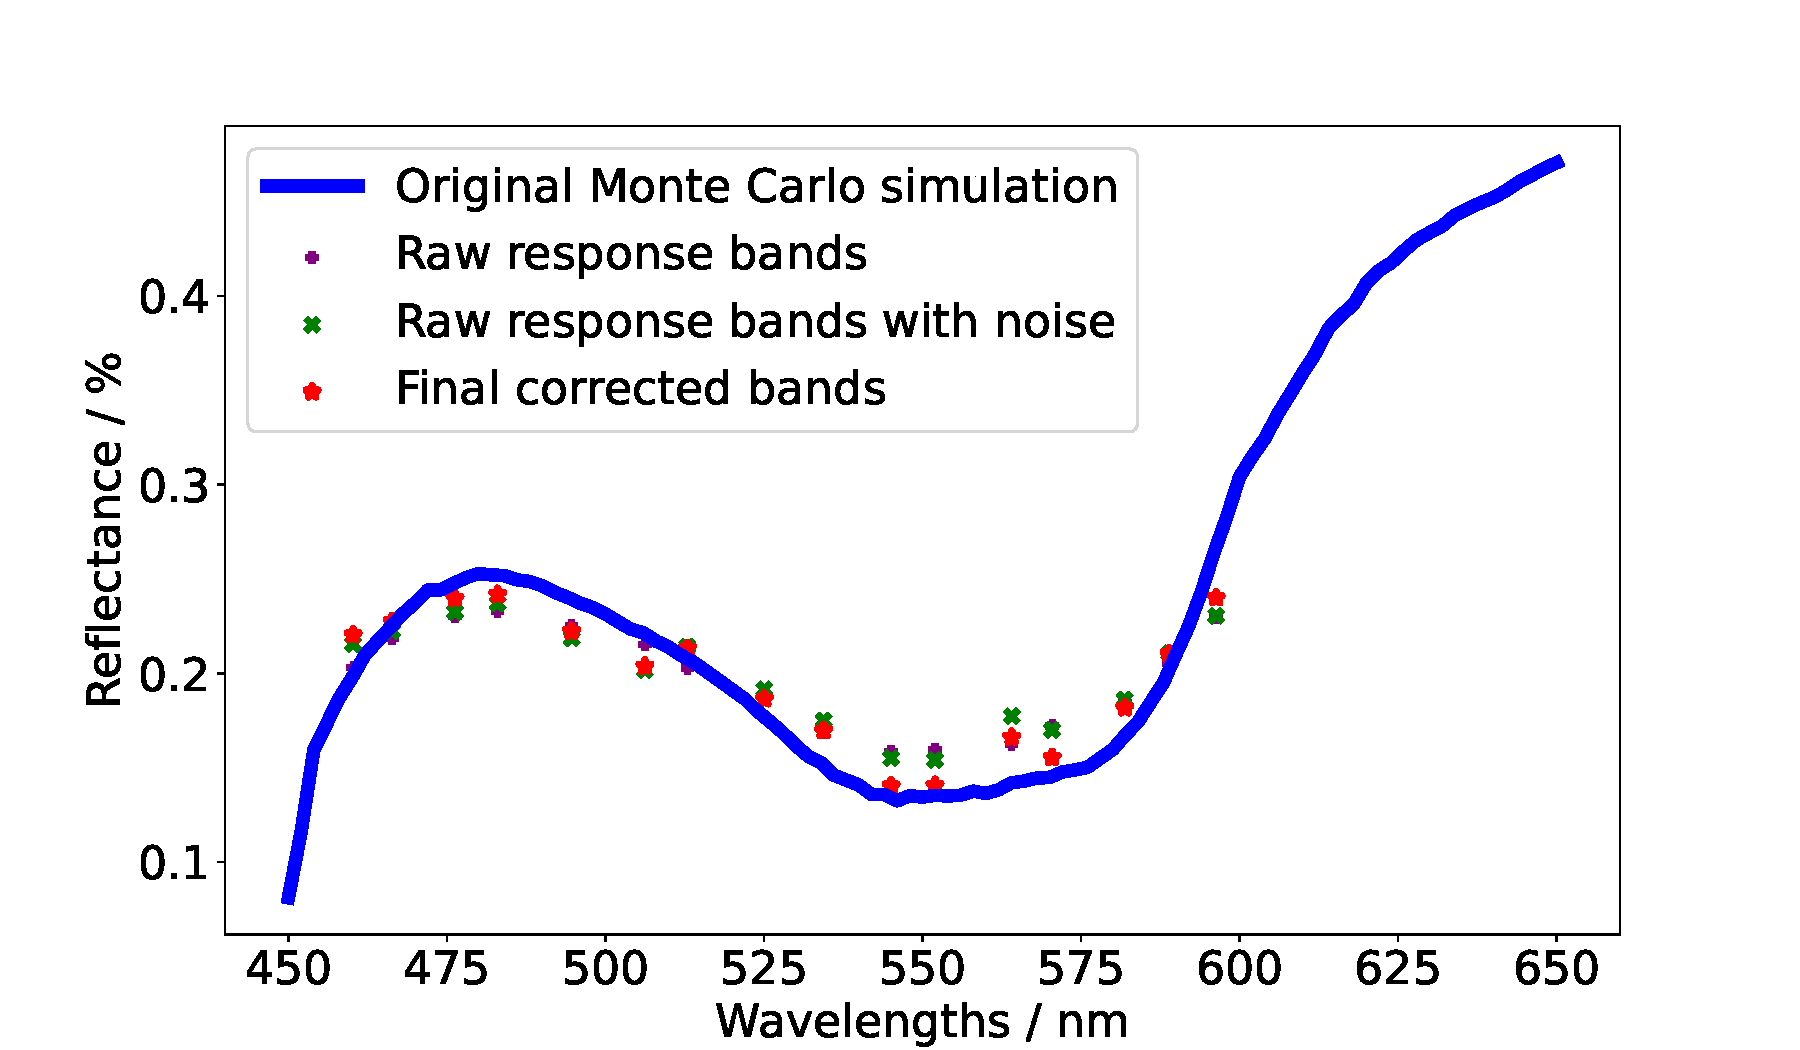
\includegraphics[width=\textwidth]{simulatingcam.pdf}
        \caption{}
        \label{fig:simulatingcamsubfigure}
    \end{subfigure}
    \begin{subfigure}{0.62\textwidth}
        \centering
        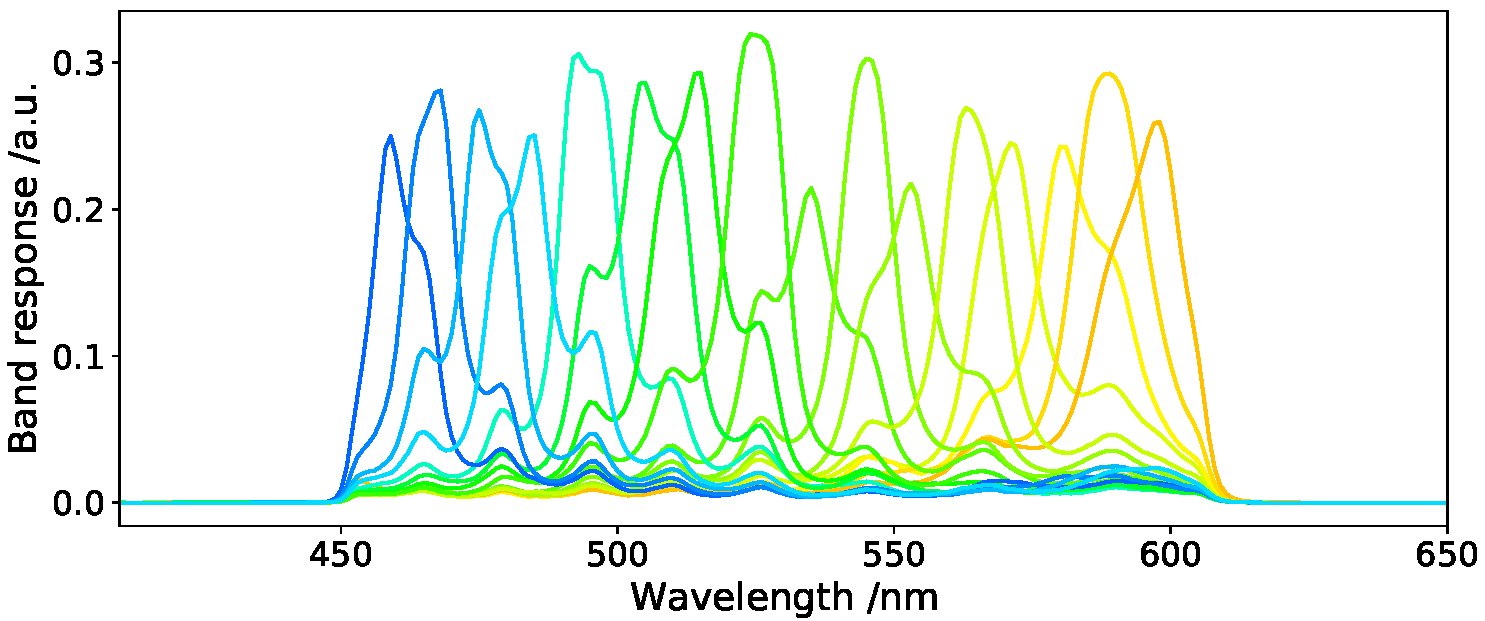
\includegraphics[width=\textwidth]{band_responses.pdf}
        \caption{}
        \label{fig:bandresponses}
    \end{subfigure}
    % 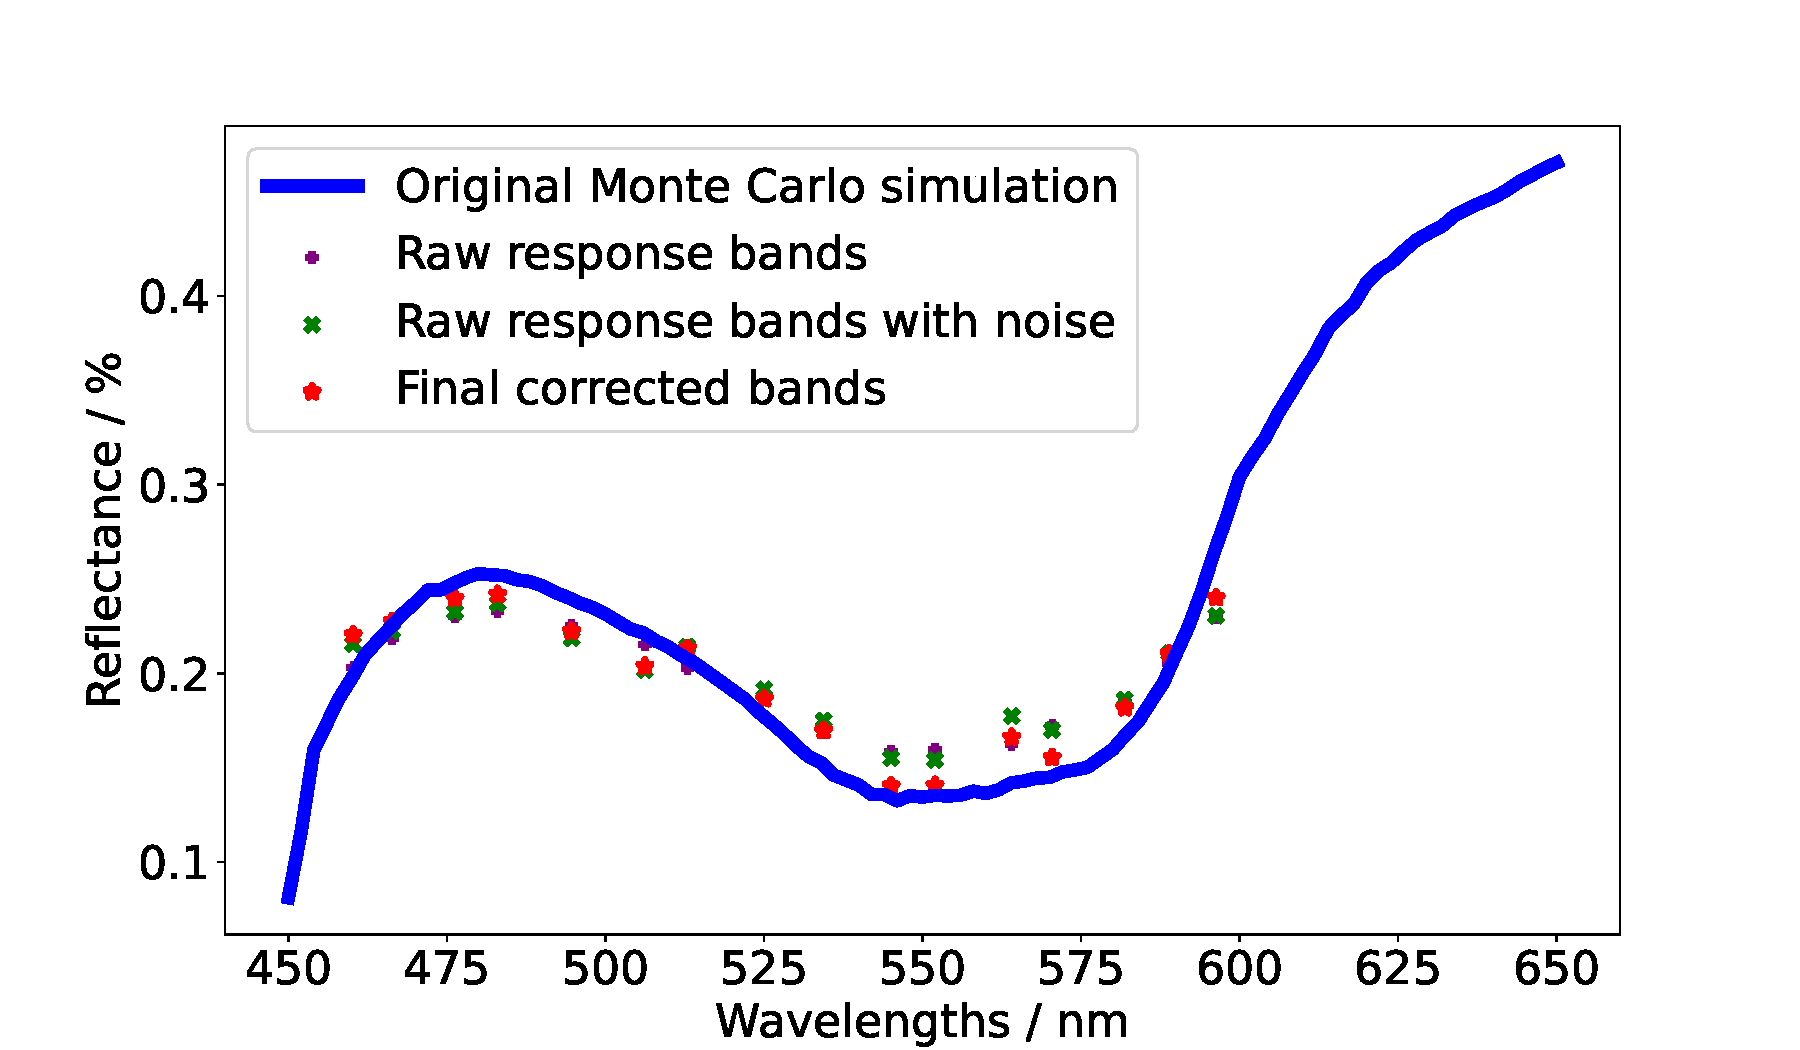
\includegraphics[width=0.7\textwidth]{simulatingcam.pdf}
    \caption{Top: An example of the stages of converting a Monte Carlo diffuse reflectance spectrum (\textcolor{blue}{blue solid}) to a simulated camera response (\textcolor{red}{red $*$}) via the band response convolution (\textcolor{purple}{purple $+$}), the noise addition (\textcolor{MyGreen}{green $\times$}), and finally cross-talk correction. Bottom: A depiction of the band responses used in this camera simulation.}
    \label{fig:simulatingcam}
\end{figure}

\subsection{Hyperspectral imaging of gelatin-based phantoms}\label{sec:imagingphantoms}
To obtain a measured hyperspectral dataset with known ground truth, short static HSI videos are taken of the two-dye configuration gelatin-based phantoms detailed in Section \ref{sec:methodsphantoms}. The imaging configuration is similar to that described in Section \ref{materials} using a 4x4 16 band visible range snapshot mosaic camera (Ximea utilising the IMEC CMV2K-SSM4X4-VIS sensor, Germany) alongside an f=35mm coupler (Karl Storz, NDTec, VCam HD-F-35 - Camera Lens Adapter, Germany), a $0^\circ$ exoscope (Karl Storz Endoscopy, VITOM Telescope 0° w Integ. Illuminator, UK) and a Xenon light source (Karl Storz Endoscopy, Cold Light Fountain D light C, UK), as detailed in \citet{Ebner2021} and pictured in Figure \ref{fig:imagephantoms}.
\begin{figure}[h!]
    \centering
    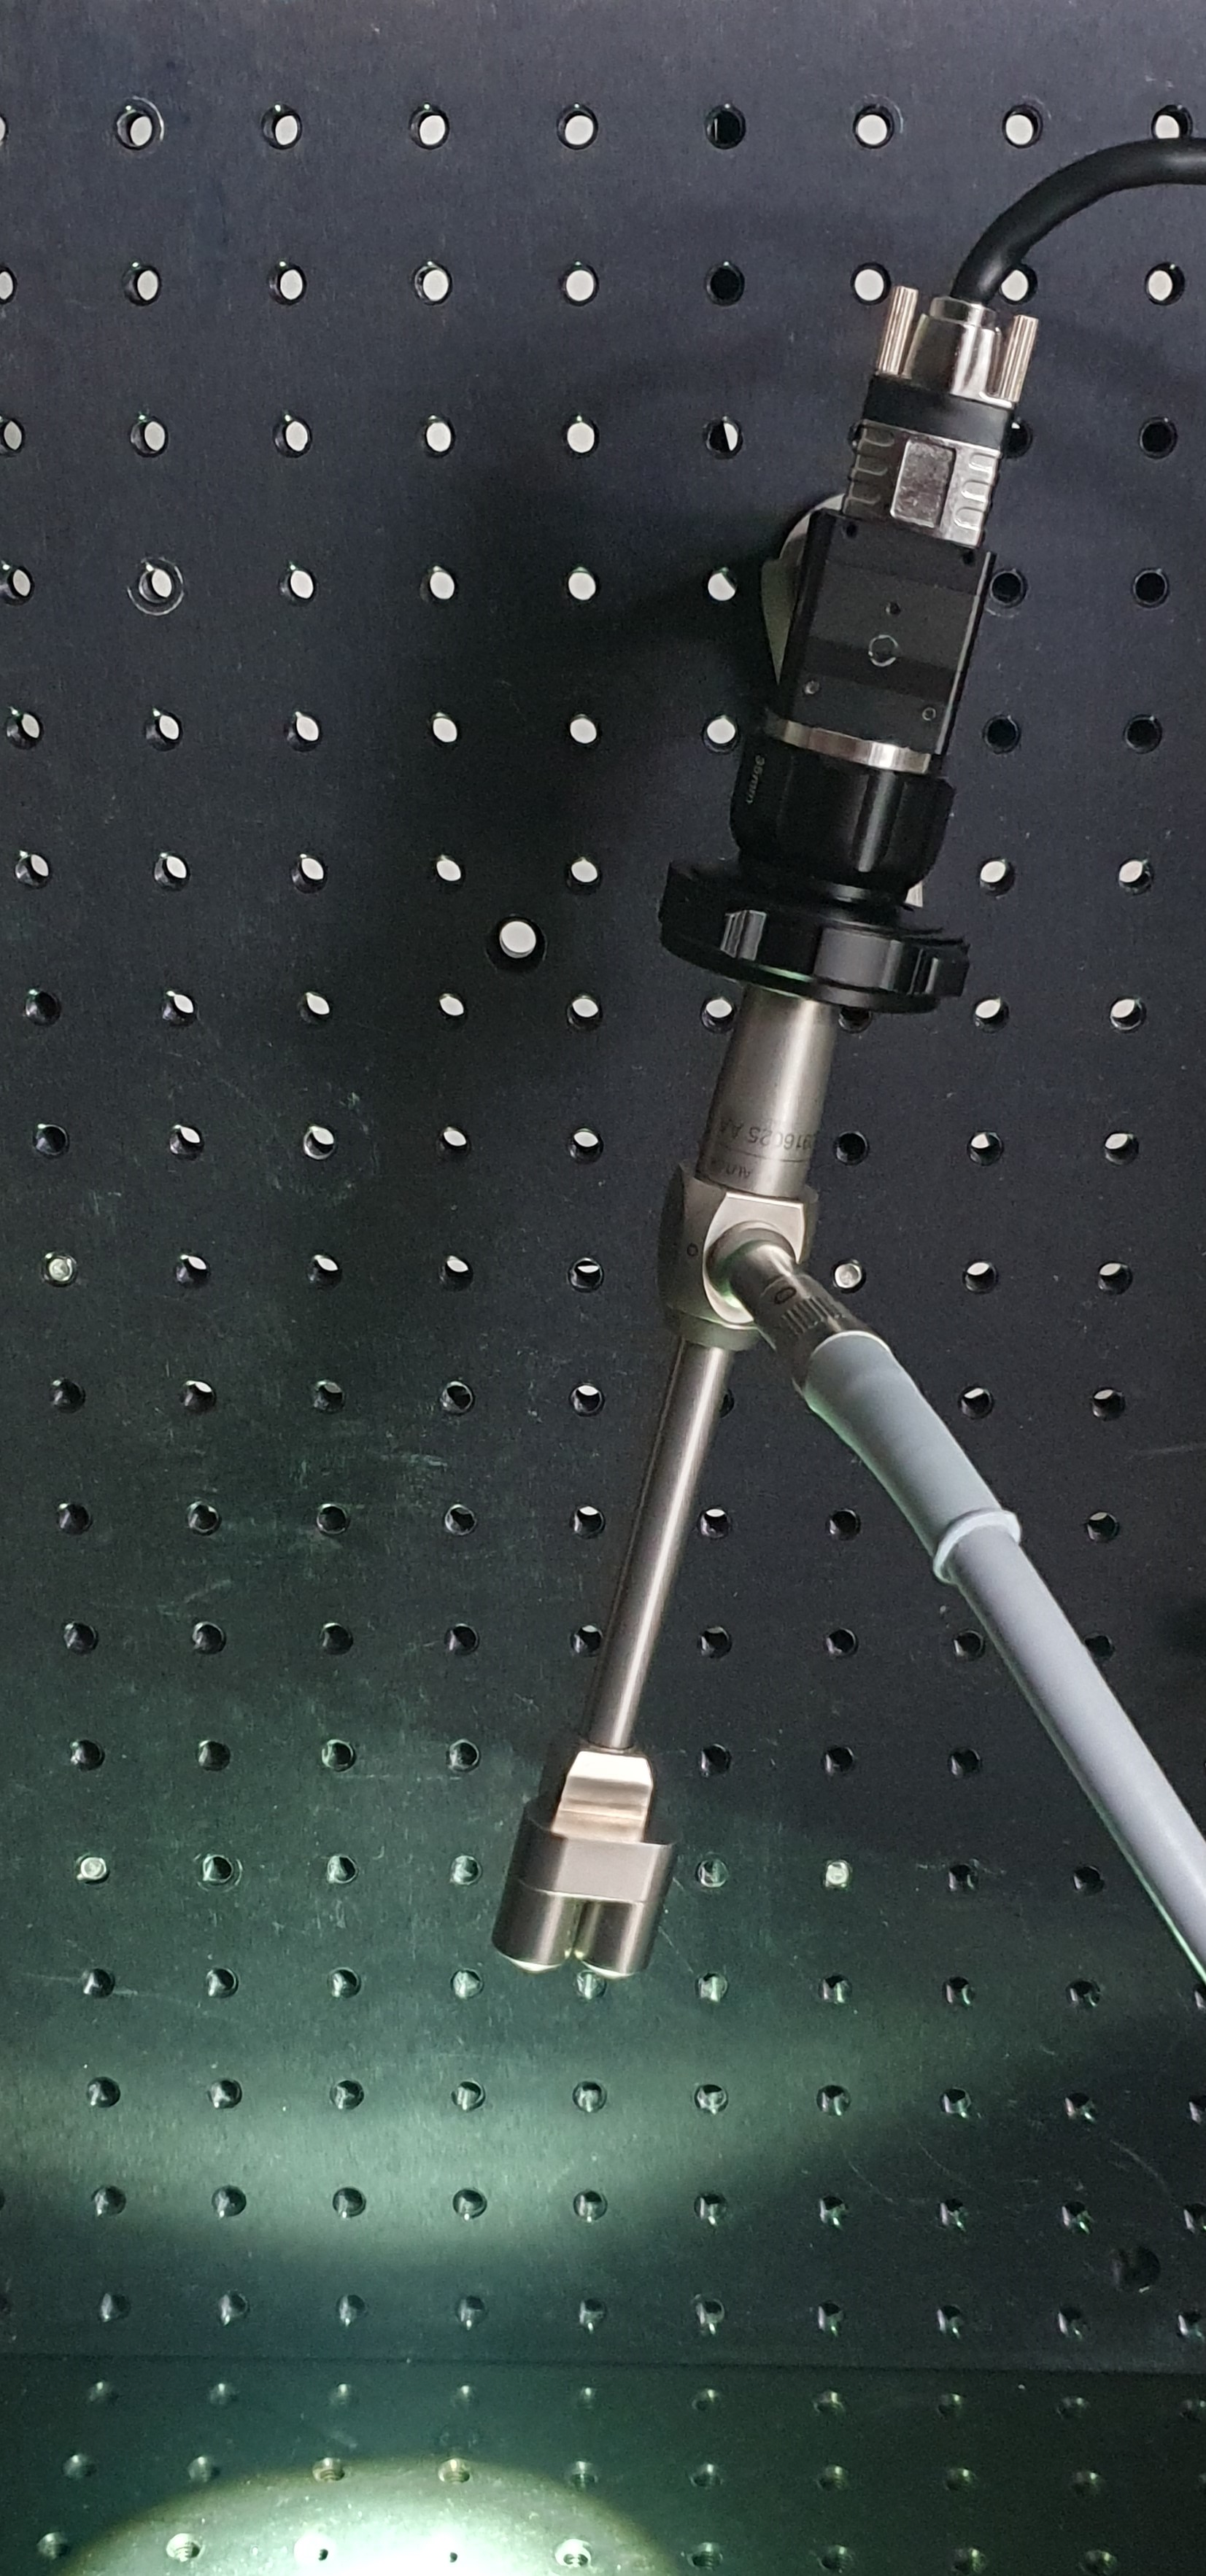
\includegraphics[width=0.3\textwidth]{imagephantoms.jpg}
    \caption{Depiction of hyperspectral imaging set-up used to acquire images of gelatin-based tissue phantoms.}
    \label{fig:imagephantoms}
\end{figure}
The configurations imaged are detailed in Table \ref{tb:imagedphantoms} and cover the majority of the 2-dye configuration dataset that remained viable after two weeks of refrigeration. 
\begin{table}[ht!]
    \centering
    \caption{Table displaying the percentages of dyes [acid red 1 (AR1), acid red 14 (AR14), crystal violet (CV)] a used for each dye configuration alongside the total dye scaled concentration in arbitrary units. The intralipid (v/v \%) imaged for each configuration are also indicated.}
    \begin{tabular}{|c|c|c|c|c|c|c|c|}
        \hline
        Total dye scaled & \multicolumn{2}{|c|}{Dye } & \multicolumn{5}{c|}{Intralipid } \\
        concentration & \multicolumn{2}{|c|}{percentage} & \multicolumn{5}{c|}{concentrations (v/v \%)} \\
        (arbitrary units) & AR1 & AR14 & 1.0 & 2.25 & 3.5 & 4.75 & 6 \\
        \hline
        1 & 50 & 50 & & x & x & x & \\
        10 & 100 & 0 & x & x & x & x & x \\
        10 & 75 & 25 & x & x & x & x & x \\
        10 & 50 & 50 &  & x & x & x & x \\
        10 & 25 & 75 & x & x & x & x & x \\
        10 & 0 & 100 & x & x &  & x & \\
        20 & 50 & 50 &  & & x & x &  \\
        \hline
    \end{tabular}
    \label{tb:imagedphantoms}
\end{table}
A white reference of a Spectralon tile of 95\% is taken under the same lighting conditions and imaging plane as the phantoms. This white reference is either used directly for white balancing a frame of the hyperspectral video to produce quantitative data or to generate spectral sensitivities used to construct mean normalised relative data as in Chapter \ref{chap:SWB}. This demonstrates both the highest fidelity and more realistic data processing pathways. Following this, bilinear demosaicing is used and cross-talk correction is applied per pixel of the frame also detailed in Chapter \ref{chap:SWB}. At this stage, it is possible to temporally average frames to improve the signal to noise ratio of the resulting hypercube. Finally, any pixel spectra containing values above 99.5\% or below 0.5\% are discarded to reduce the impact of specular reflections and to ensure the data is within the dynamic range of the sensor. 
Each image is manually annotated using ImFusion Labels software to capture pixels corresponding to phantoms while avoiding regions with high specular reflection. This allows a mean spectrum of the phantom to be generated and compared per pixel processing of the annotated region. When using this data only wavelengths in the region 450-575nm are considered (i.e. 13 of the 16 bands of the camera), since Chapter \ref{chap:1layer} demonstrated this to be the optimum fitting region for these phantoms. 

\subsection{Neurosurgical HSI dataset}\label{sec:NeuroHSIdata}
The HELICoiD dataset is leveraged in this work which captures data in the wavelength range 400-1000nm using a pushbroom spatial scanning HSI camera~\citep{Fabelo2019}. This data is obtained as part of a collaboration between four universities, three industrial partners, and two hospitals in the European Union~\citep{Fabelo2019}. This provides 36 high spectral resolution images of 22 patients which are annotated with use of spectral angle mapper to identify four key classes: "normal tissue, tumour tissue, blood vessel, and background elements". This data is white balanced using associated flatfield white references included in the dataset. The resulting spectra are then normalised to reduce the impact of any differences in relative position of the camera to the data and white reference as discussed in Chapter \ref{chap:SWB}. For this work we consider only the spectral range of 450-600nm as this is the range of use for the analytical models considered. 
%Secondly, a NeuroHSI dataset is considered which is obtained using the same snapshot mosaic camera (Ximea utilising the IMEC CMV2K-SSM4X4-VIS sensor, Germany) as in Section \ref{sec:imagingphantoms} whose bands are within the 450-600nm wavelength range. In contrast to Section \ref{sec:imagingphantoms}, this is mounted to a neurosurgical microscope (Zeiss Kinevo 900, Germany) whose integrated light source and lenses are used for simpler integration into the neurosurgical workflow, allowing for use in a wide variety of neurosurgical cases. 
%%This light source and optical system was not fully characterised and therefore the vignetting profile cannot be assumed to follow the trends seen in Chapter \ref{chap:SWB} and so the full white balancing algorithm using the sterile ruler cannot be implemented for quantitative data. In it's place, 
%In each imaging timepoint of this study, the position of the neurosurgical microscope is recorded and used to obtain a flatfield reference outside the sterile field in a closely correlated position and lighting conditions. Due to the significant curvature of the brain, this may not accurately account for the full vignetting profile so is not used for flatfield correction to produce quantitative data, and instead is used to generate spectral senstivities for relative data before demosaicing, cross-talk correction, and removal of spectra containing values above 99.5\% or below 0.5\%. These spectral sensitivities are found to be similar to those pre-calculated from the light source spectrum. This dataset is manually annotated using ImFusion Labels software to identify over 30 classes. 

When fitting inverse models to these datasets we use a wavelength weighting similar to that seen in Chapter \ref{chap:2layer} and reproduced in Figure \ref{fig:weightings}, however analysis with uniform wavelength weighting can be seen in Appendix \ref{ap:Chapter5uniform}. We also investigate two different fitting regimes where either the literature extinction coefficients for oxygenated and deoxygenated haemoglobin are used, or these extinction coefficients are shifted by 3nm before use. This 3nm shift was determined empirically as that which aligns with the peak positions seen in the HELICoiD mean annotated spectra. This difference in peak positions is likely driven by imperfect wavelength calibration in the HELICoiD system, however it could also arise from the difference in chemical environment of the haemoglobin in biological tissue compared to the acqueous configuration the literature values are measured in as mentioned for the dyes used in Chapter \ref{chap:1layer}. The literature and shifted extinction coefficients can be seen in Figure \ref{fig:extinctioncoeffs}.
% \begin{enumerate}
%     \item Wavelengths (450 - 600nm) are considered equally in the fitting of the residual. Literature extinction coefficients are used for oxyenated and deoxyenated haemoglobin. 
%     \item All wavelengths (450 - 600nm) are considered in the fitting of the residual, however those in the region of the haemoglobin peaks (525 - 585nm) are considered more heavily. Literature extinction coefficients are used for oxyenated and deoxyenated haemoglobin. 
%     \item Wavelengths (450 - 600nm) are considered equally in the fitting of the residual. Literature extinction coefficients for oxyenated and deoxyenated haemoglobin are shifted by 3nm before use. 
%     \item All wavelengths (450 - 600nm) are considered in the fitting of the residual, however those in the region of the haemoglobin peaks (525 - 585nm) are considered more heavily. Literature extinction coefficients for oxyenated and deoxyenated haemoglobin are shifted before use.
%     \label{ls:fittingmethods}
% \end{enumerate}
% The wavelength weightings and extinction coefficients are shown in Figure \ref{fig:fittingoptions}. 
\begin{figure}[h!]
    \centering
    \begin{subfigure}{0.49\textwidth}
        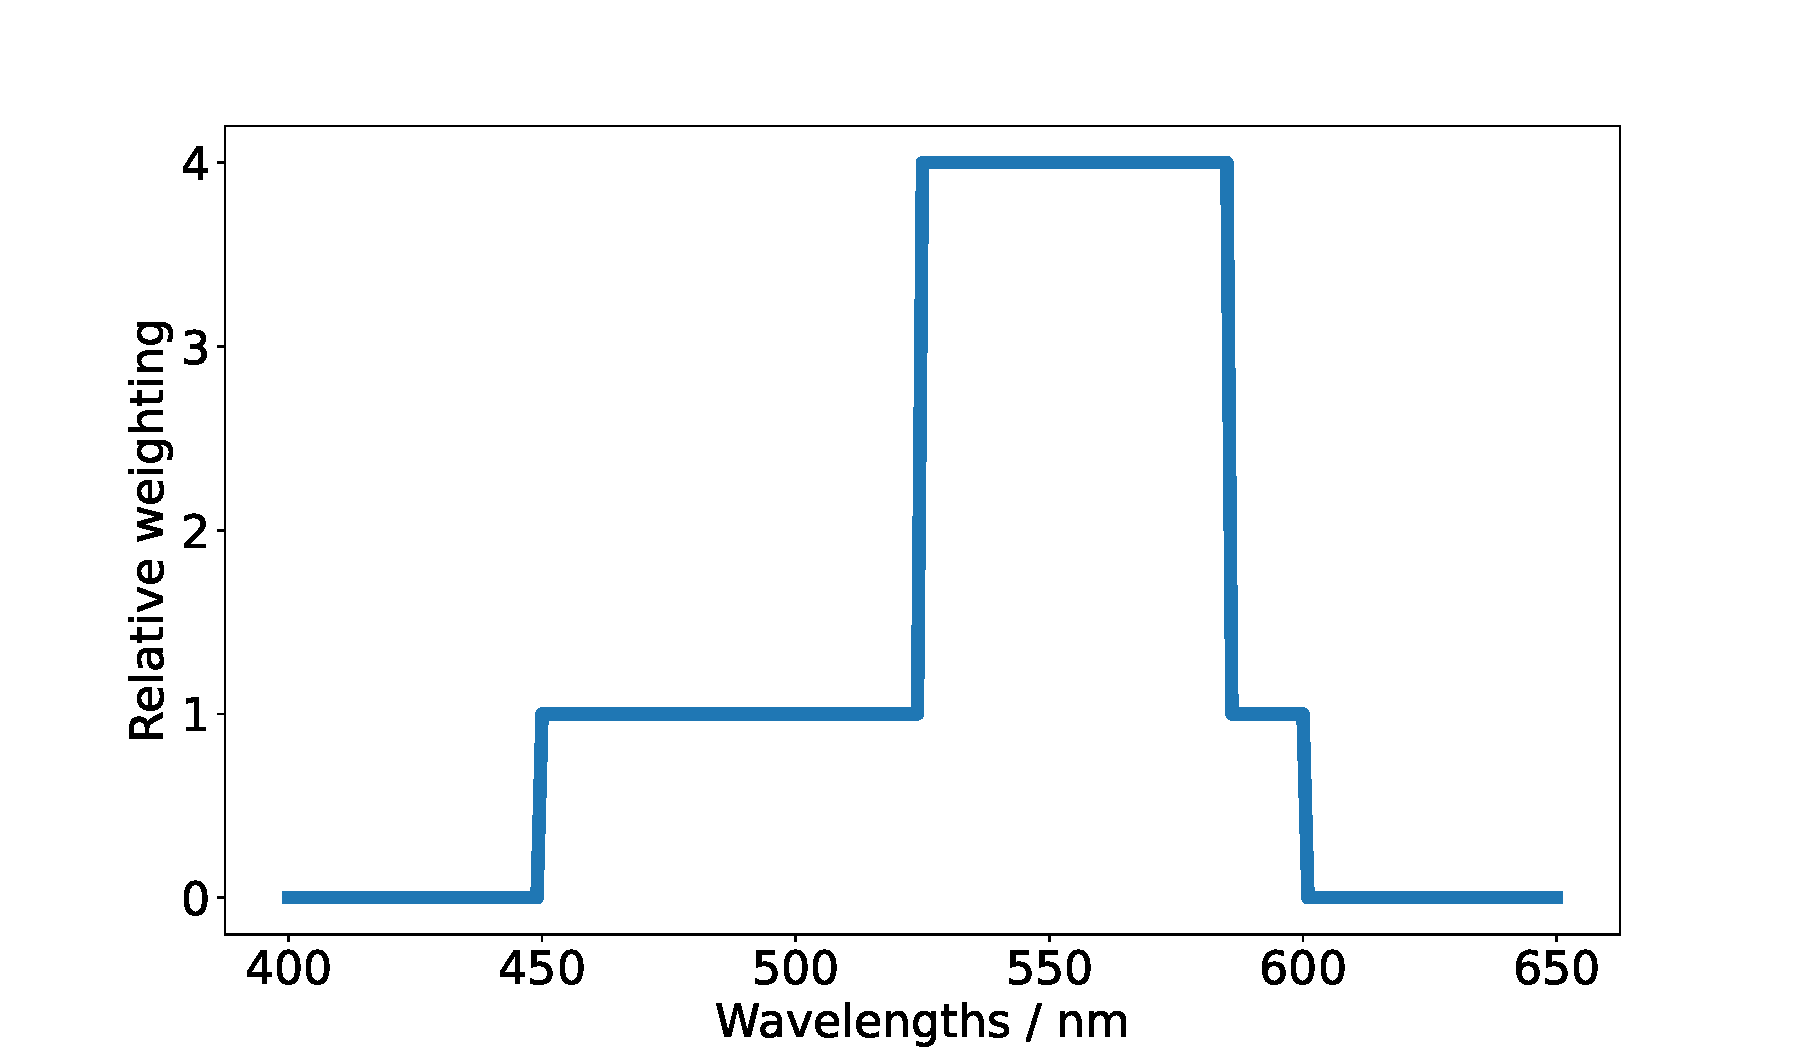
\includegraphics[width=\textwidth]{fitting_region.pdf}
        \caption{}
        \label{fig:weightings}
    \end{subfigure}
    \begin{subfigure}{0.49\textwidth}
        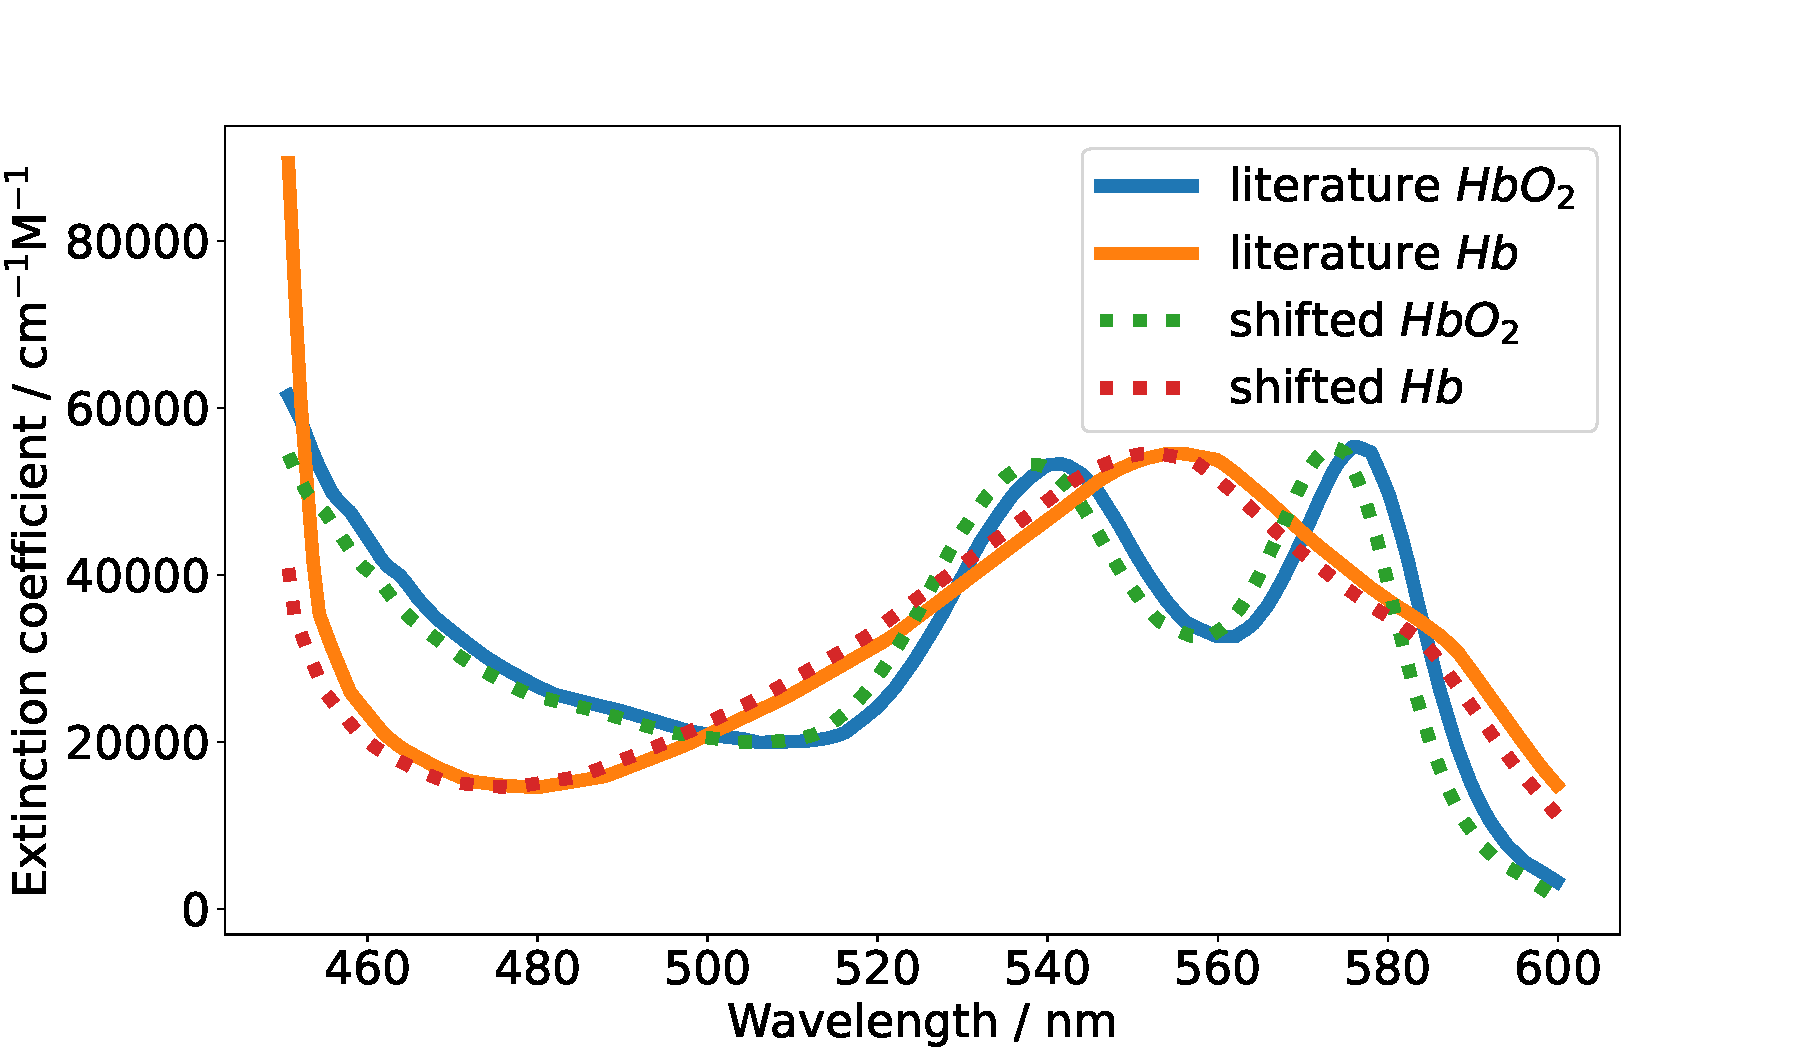
\includegraphics[width=\textwidth]{extinction_coefficients.pdf}
        \caption{}
        \label{fig:extinctioncoeffs}
    \end{subfigure}
    \caption{Wavelength weighting (left) and extinction coefficient (right) options used to fit models to neurosurgical HSI data.}
    \label{fig:fittingoptions}
\end{figure}

\subsection{Evaluation of analytical models}
The Yudovsky 2009 single and double layer models and Jacques 1999 models are evaluated as these are found to be the most effective in Chapters \ref{chap:1layer} and \ref{chap:2layer}. These models are evaluated against datasets generated by simulating camera responses from the dermal and skin Monte Carlo datasets used in Chapters \ref{chap:1layer} and \ref{chap:2layer} and so the diffuse reflectance prediction of these models are unchanged in this Chapter. When using these analytical models with the snapshot HSI datasets outlined in Sections \ref{sec:MCcameras} to \ref{sec:NeuroHSIdata}, the predicted $R$ (detailed in Sections \ref{sec:Jacques}, \ref{sec:Yudovskysingle}, and \ref{sec:Yudovsky2009}) is used to simulate noiseless camera responses as described by Equation \eqref{eq:simulatingcam}. This simulation is not performed for the HELICoiD dataset as the camera band responses are not available in the dataset, however the authors report a very low dispersion of 0.74nm in the spectral range considered in this work so it is likely that the camera simulation would not have as significant of an impact with this system~\citep{Fabelo2018}. This allows the forwards and fitted models to be evaluated and quantified as described in Sections \ref{sec:methodevaluate} and \ref{sec:methodevaluate2} against the Monte Carlo datasets, and similarly for the single-layer models for the gelatin-based phantom datsets. 

For the gelatin-based phantom datasets, either the mean spectrum of the annotated region of a single frame is used, or each pixel in an annotated region from a single frame or from the temporal averaging of 5 frames is used. Both spatial and temporal averaging reduces the impact of noise on the resulting data. The mean annotated spectra are used for fitting the models (using the wavelength range 450-575nm) or to evaluate the quality of the forwards models with camera simulation. The quality of camera simulation can also be evaluated using $NRMSE$ and Pearson correlation coefficients by comparing simulated camera spectra from the spectrophotometer measurements of the gelatin-based phantoms in Section \ref{sec:methodsphantoms}, to the measured HSI data in Section \ref{sec:imagingphantoms}. The pixel-by-pixel analysis of the annotated region of either a single frame or the temporal average of 5 frames is used for fitting models to allow for spatially resolved results.

Finally, for each neurosurgical dataset image, the mean spectrum of each class annotation is calculated and the inverse analytical models are fitted to this (using the wavelength range 450-600cm). This provides a set of physiological parameters for each class of each image which are then collated to provide a range of values which are considered for plausibility. % Need to find better academic phrasing here 

The most effective model is chosen to evaluate exemplary HELICoiD and phantom images on a pixel-by-pixel level. Where a phantom image is evaluated, the $APE$ of $AR1$ compared to the ground truth value is also displayed; however, where a HELICoiD image is evaluated the $APE$ of $StO_2$ compared to that obtained from the mean annotated spectrum is shown for pixels within the annotated regions. 

\section{Results}

\subsection{Monte Carlo}\label{sec:MCHSI}
The forwards analytical models are assessed using simulated camera responses generated from Monte Carlo data. 
%The Yudovsky 2009 and Jacques 1999 single-layer models are evaluated for three refractive indices, whereas the Yudovsky 2009 double-layer model is evaluated for $n=1.44$ only as in Chapters \ref{chap:1layer} and \ref{chap:2layer}. 
These are evaluated in Table \ref{tb:forwardsHSIMC} for $n=1.44$ (further refractive indices can be found in Appendices \ref{ap:forwardsHSIMCq} and \ref{ap:forwardsHSIMCr}). Examples of the quality of fitting for the single and double layer configurations with noiseless camera simulations are shown in Figure \ref{fig:forwardsHSIMC}. Visual examples of the impact of noise on simulated MC spectra are seen in Figure \ref{fig:forwardsMCnoise}.
\begin{table}[h!] %could remove noise levels here
    \centering
    \caption{Mean (standard deviation) $NRMSE$ (3.d.p.) between the simulated camera responses of each forwards spectrum from each model and each of 100 Monte Carlo simulated spectra using the same ground truth variable parameters for quantitative and relative data at a variety of noise levels (0, 1pp, 3pp). This is presented with the Pearson $r$ (bold if Pearson $p < 0.05$) for the linear regression between all forwards spectra against Monte Carlo simulated spectra for each refractive index dataset and each analytical model. All metrics are evaluated for the wavelength region of 450-600nm.}
    \begin{tabular}{|cc|c|ccc|ccc|}
        \hline
        Model & Layers & Quantitative & \multicolumn{3}{|c}{$NRMSE$} & \multicolumn{3}{|c|}{$r$} \\
         & & (Q) or & 0pp & 1pp & 3pp & 0pp & 1pp & 3pp \\
         & & Relative (R) &  &  &  &  & &  \\
        \hline
        \multirow{2}{*}{\shortstack{Yudovsky\\ 2009}} & \multirow{2}{*}{1} & Q & \shortstack{0.009 \\(0.004)} & \shortstack{0.082 \\(0.057)} & \shortstack{0.224 \\(0.125)} & \textbf{1.000} & \textbf{0.993} & \textbf{0.942} \\
        & & R & \shortstack{0.003 \\(0.002)} & \shortstack{0.075 \\(0.044)} & \shortstack{0.212 \\(0.118)} & \textbf{1.000} & \textbf{0.916} & \textbf{0.602} \\
        \hline
        \multirow{3}{*}{\shortstack{Jacques\\ 1999}} & \multirow{2}{*}{1} & Q & \shortstack{0.026 \\(0.046)} & \shortstack{0.089 \\(0.077)} & \shortstack{0.227 \\(0.130)} & \textbf{1.000} & \textbf{0.993} & \textbf{0.942} \\
        & & R & \shortstack{0.014 \\(0.021)} & \shortstack{0.076 \\(0.045)} & \shortstack{0.212 \\(0.117)} & \textbf{0.995} & \textbf{0.915} & \textbf{0.605} \\
        \hline
        \multirow{2}{*}{\shortstack{Yudovsky\\ 2009}} & \multirow{2}{*}{2} & Q & \shortstack{0.166 \\(0.133)} & \shortstack{0.482 \\(0.289)} & \shortstack{0.738 \\(0.294)} & \textbf{0.992} & \textbf{0.971} & \textbf{0.829} \\
         &  & R & \shortstack{0.033 \\(0.026)} & \shortstack{0.428 \\(0.286)} & \shortstack{0.684 \\(0.286)} & \textbf{0.991} & \textbf{0.270} & -0.007 \\
        \hline
    \end{tabular}
    \label{tb:forwardsHSIMC}
\end{table}

\begin{figure}[h!]
    \centering
    \begin{subfigure}{0.49\textwidth}
        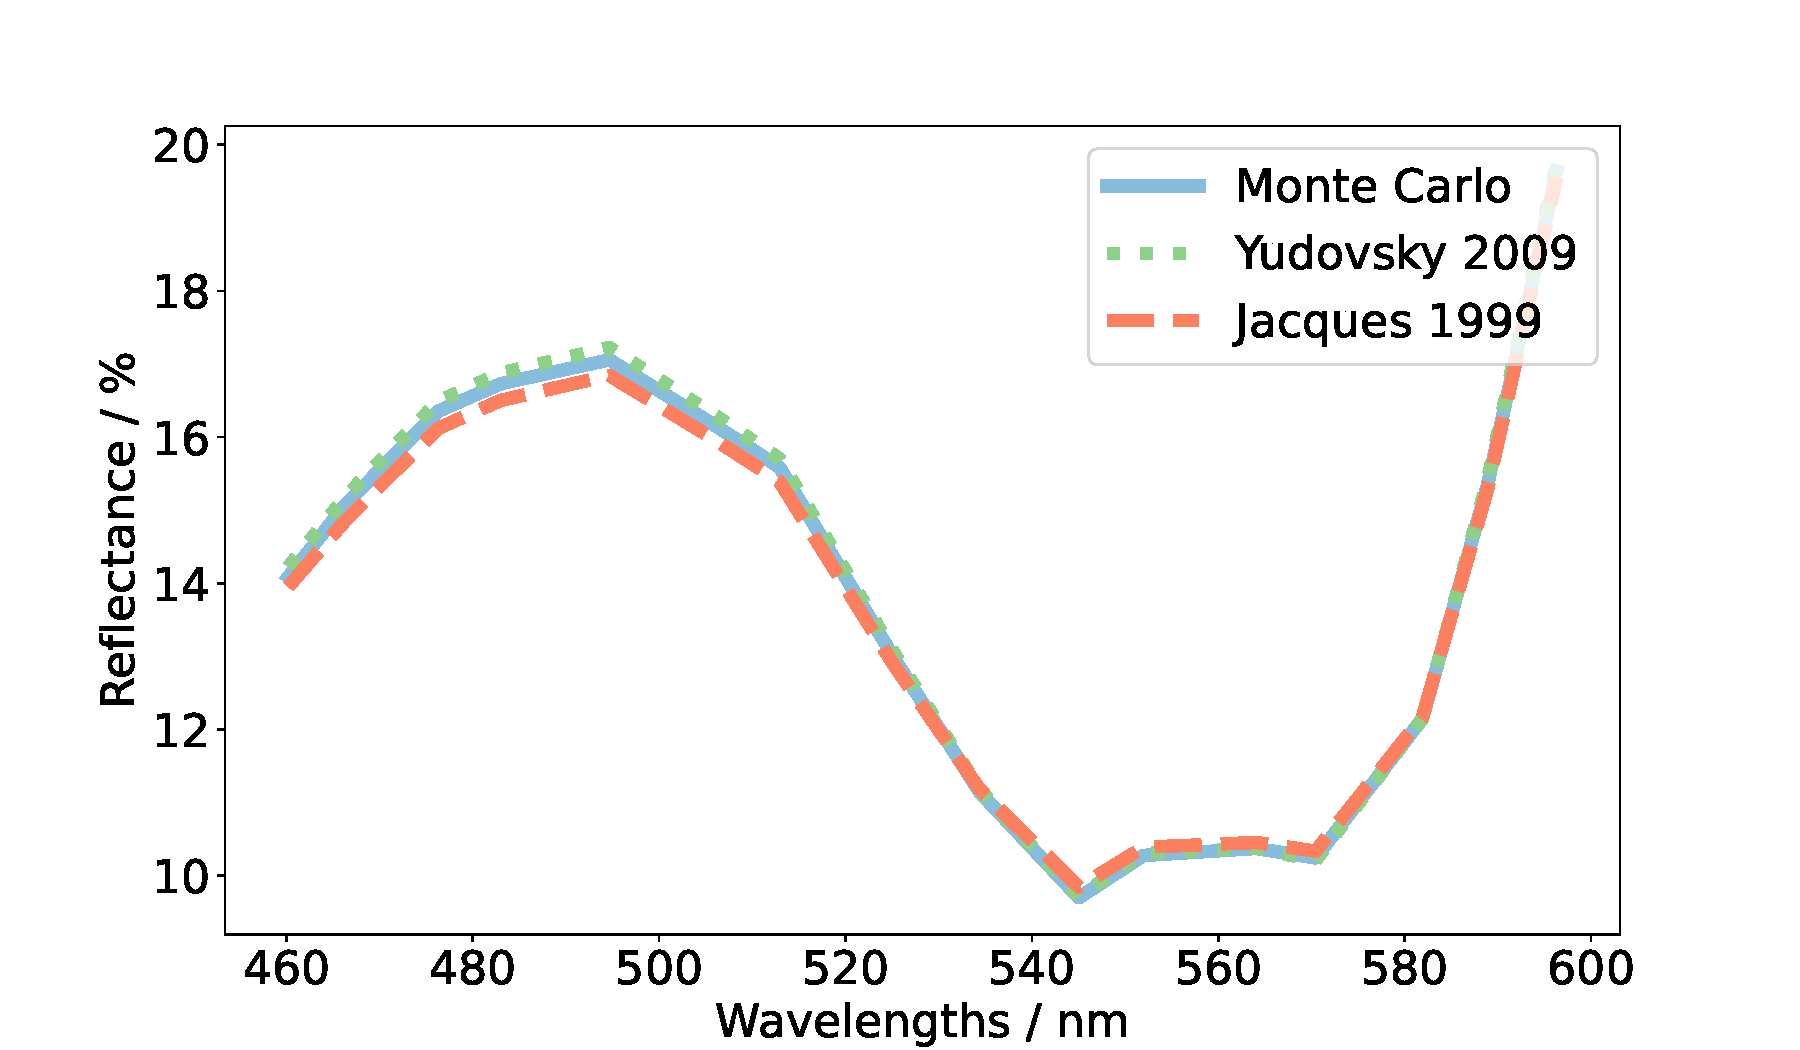
\includegraphics[width=\textwidth]{forwards_cam_Q.pdf}
        \caption{}
        \label{fig:egforwardsnoiseQ}
    \end{subfigure}
    \begin{subfigure}{0.49\textwidth}
        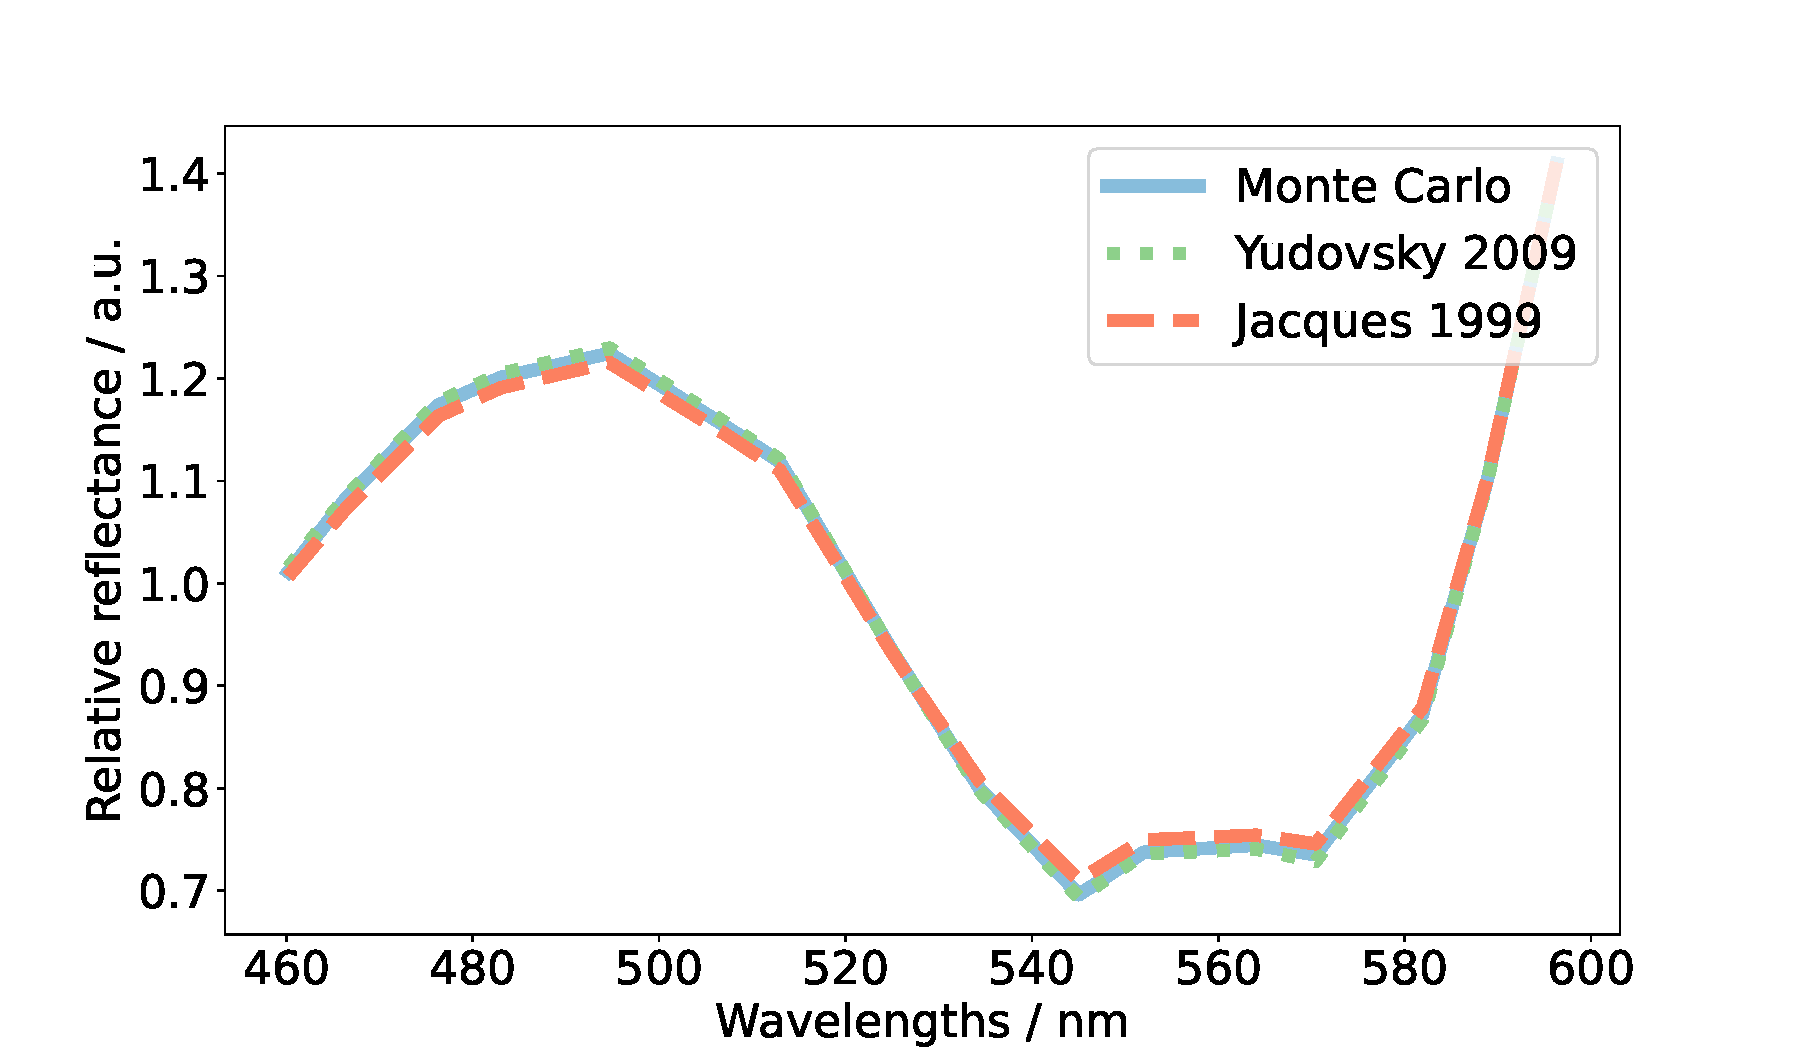
\includegraphics[width=\textwidth]{forwards_cam_R.pdf}
        \caption{}
        \label{fig:egforwardsnoiseR}
    \end{subfigure}
    \begin{subfigure}{0.49\textwidth}
        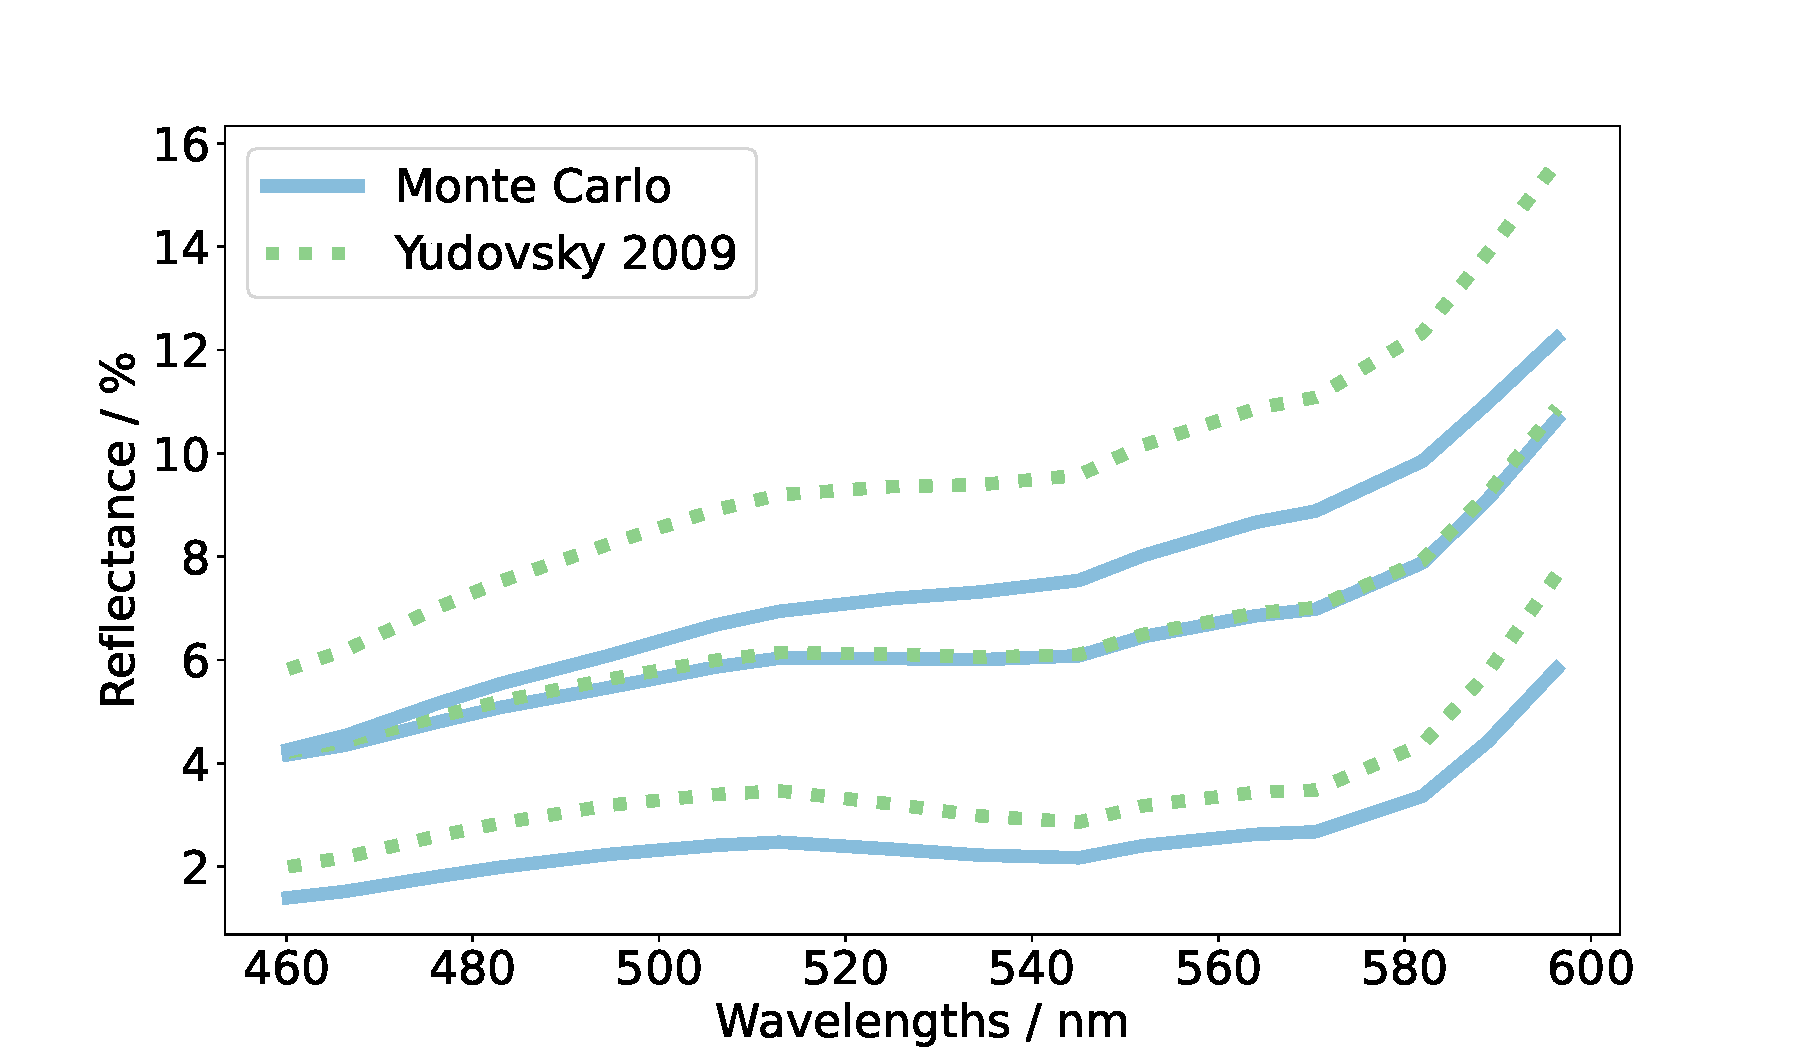
\includegraphics[width=\textwidth]{forwards_cam2_Q.pdf}
        \caption{}
        \label{fig:egforwards2noiseQ}
    \end{subfigure}
    \begin{subfigure}{0.49\textwidth}
        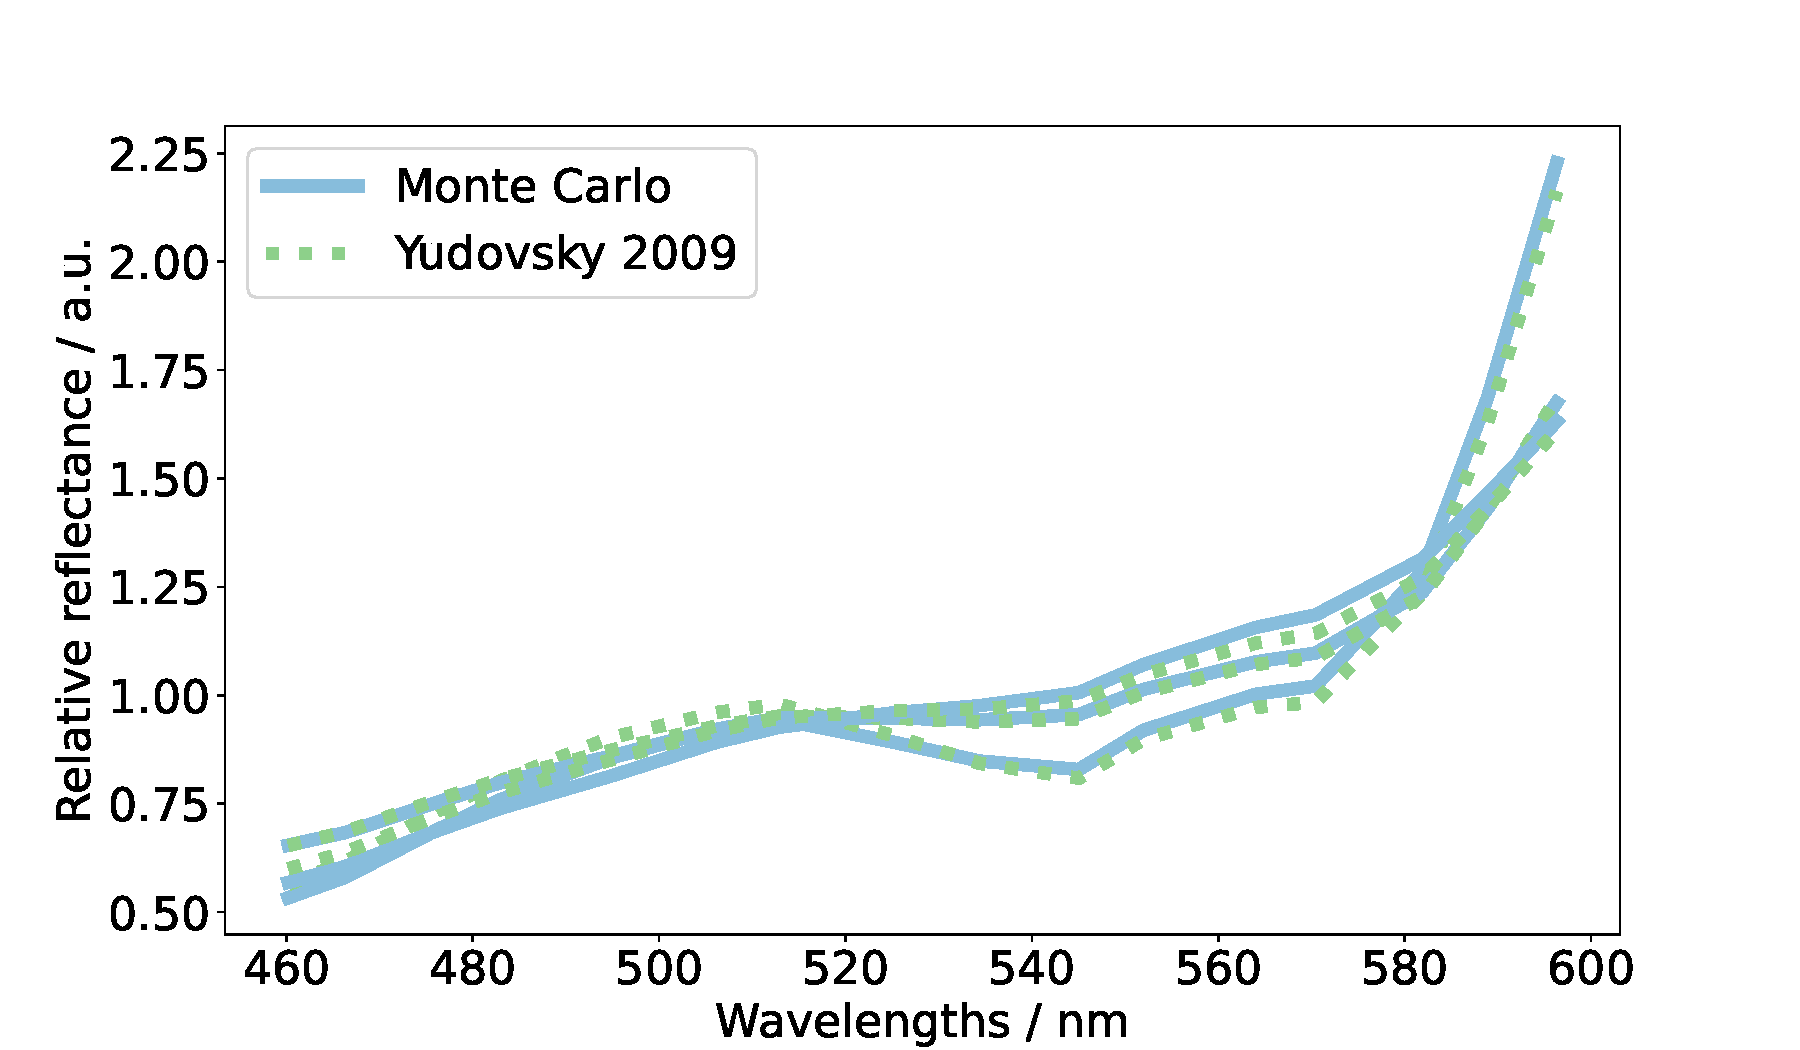
\includegraphics[width=\textwidth]{forwards_cam2_R.pdf}
        \caption{}
        \label{fig:egforwards2noiseR}
    \end{subfigure}
    \caption{Top: Example of the simulated camera response spectra from each forward single-layer analytical model: Yudovsky 2009 (\textcolor{MyGreen}{green dotted}) and Jacques 1999 (\textcolor{MyOrange}{orange dashed}), using ground truth variables for a refractive index of 1.44 compared to that predicted by Monte Carlo %with (\textcolor{purple}{purple dash-dotted} and 
    without noise added (\textcolor{MyBlue}{blue solid}) for quantitative (left) and relative (right) data. Bottom: Demonstration of the variability of quality of prediction between the simulated camera responses from the Yudovsky 2009 two layer model (\textcolor{MyGreen}{green dotted}) and Monte Carlo with %(\textcolor{purple}{purple dash-dotted} and 
    without noise added (\textcolor{MyBlue}{blue solid}) when using the same ground truth parameters for quantitative (left) or relative (right) data.}
    \label{fig:forwardsHSIMC}
\end{figure}

\begin{figure}[h!]
    \centering
    \begin{subfigure}{0.49\textwidth}
        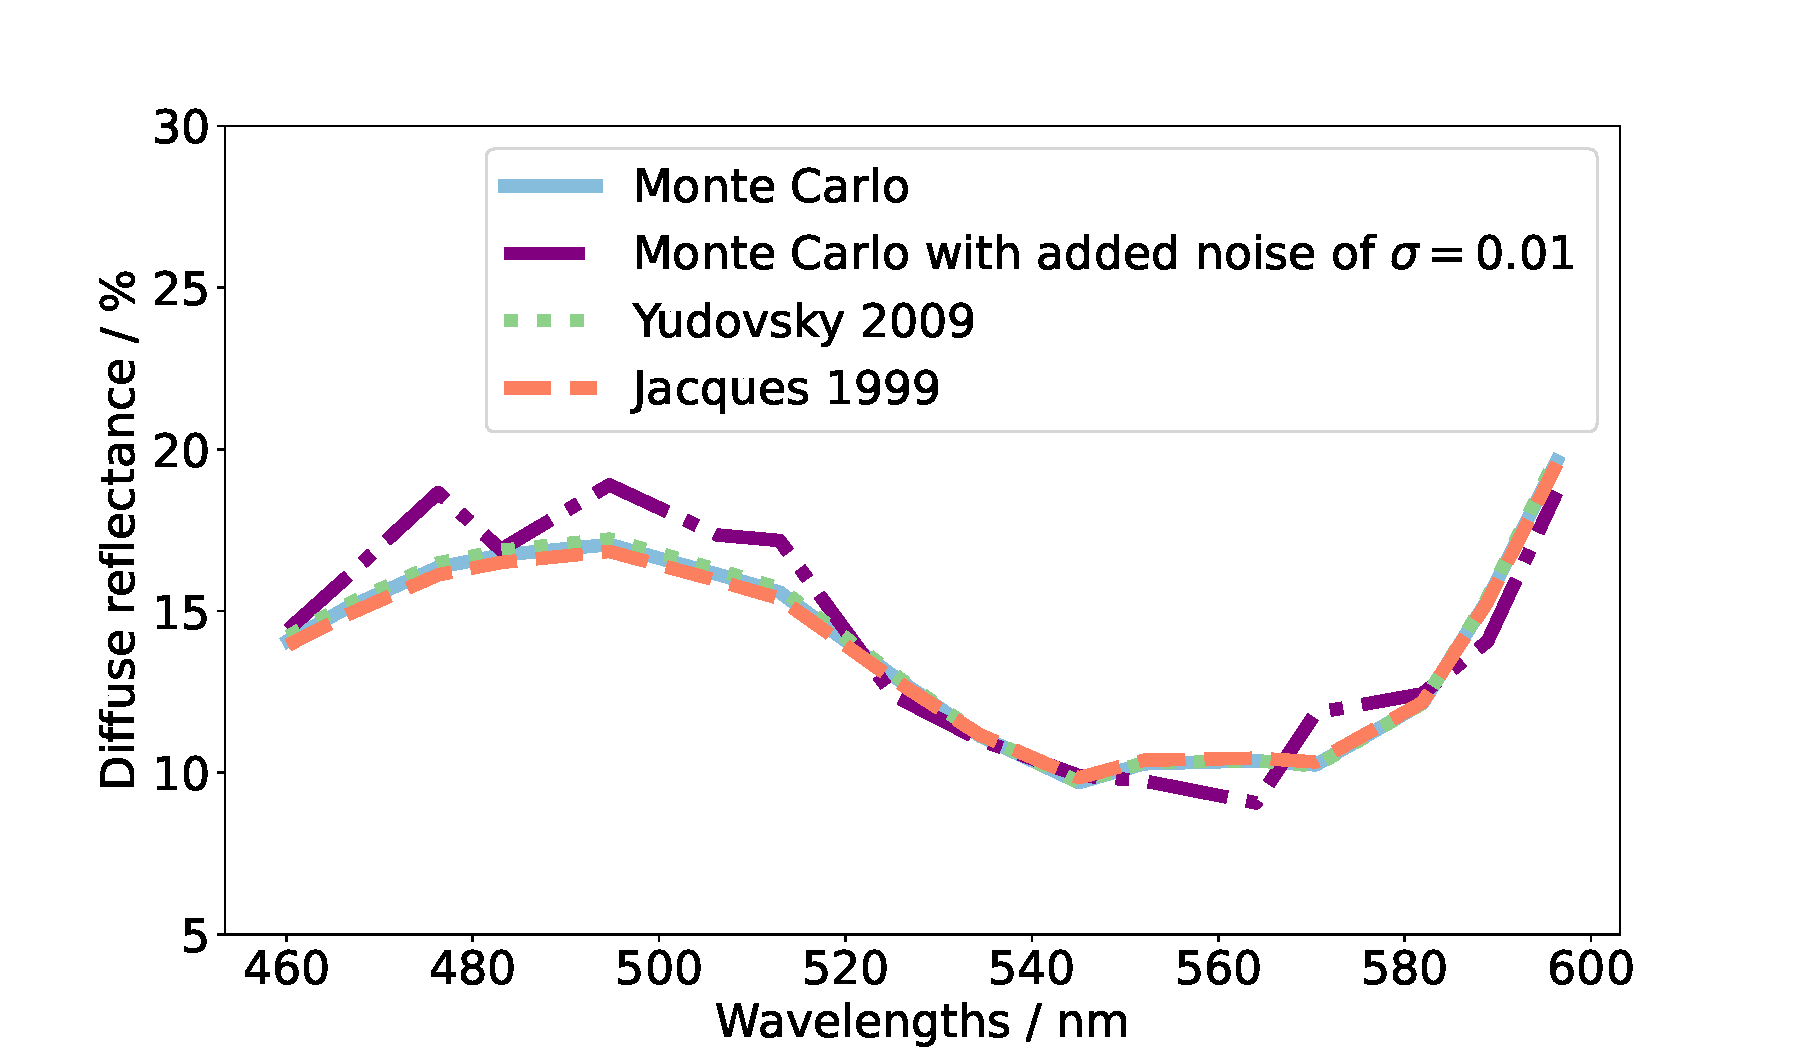
\includegraphics[width=\textwidth]{forwards_noise_Q.pdf}
        \caption{}
        \label{fig:egforwardsnoiseMCQ}
    \end{subfigure}
    \begin{subfigure}{0.49\textwidth}
        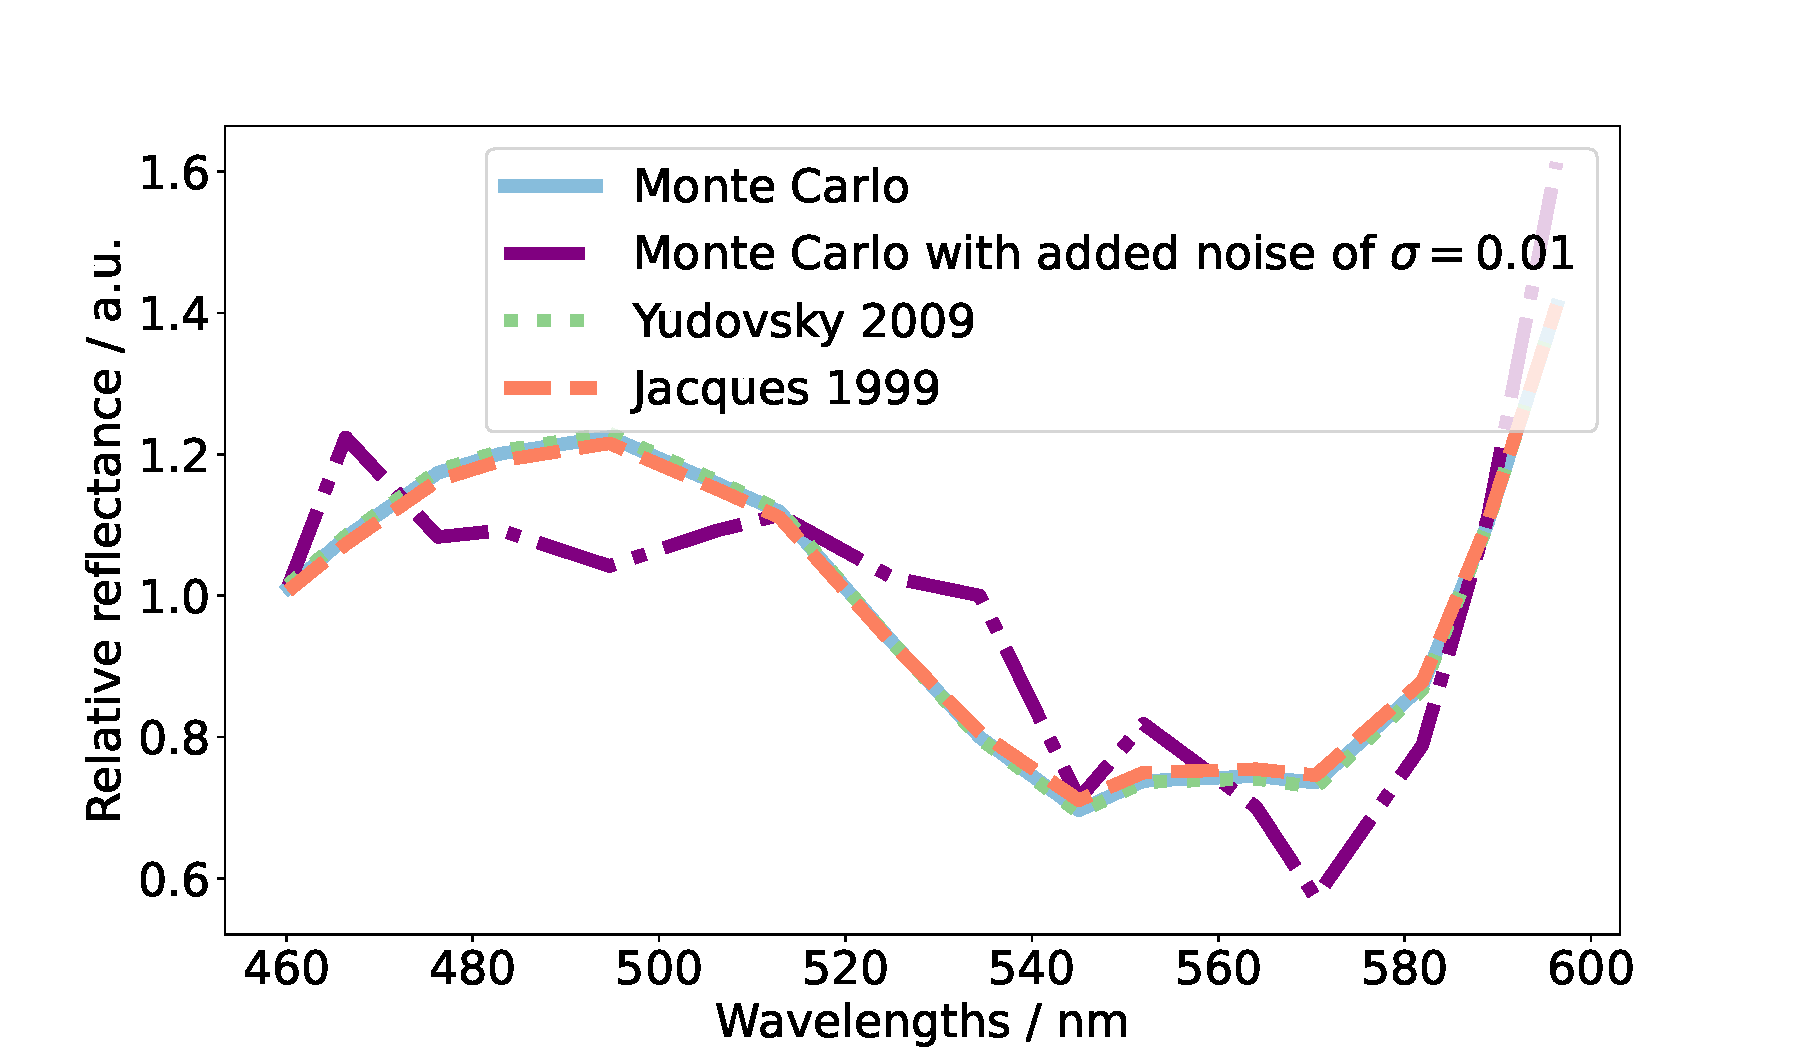
\includegraphics[width=\textwidth]{forwards_noise_R.pdf}
        \caption{}
        \label{fig:egforwardsnoiseMCR}
    \end{subfigure}
    \begin{subfigure}{0.49\textwidth}
        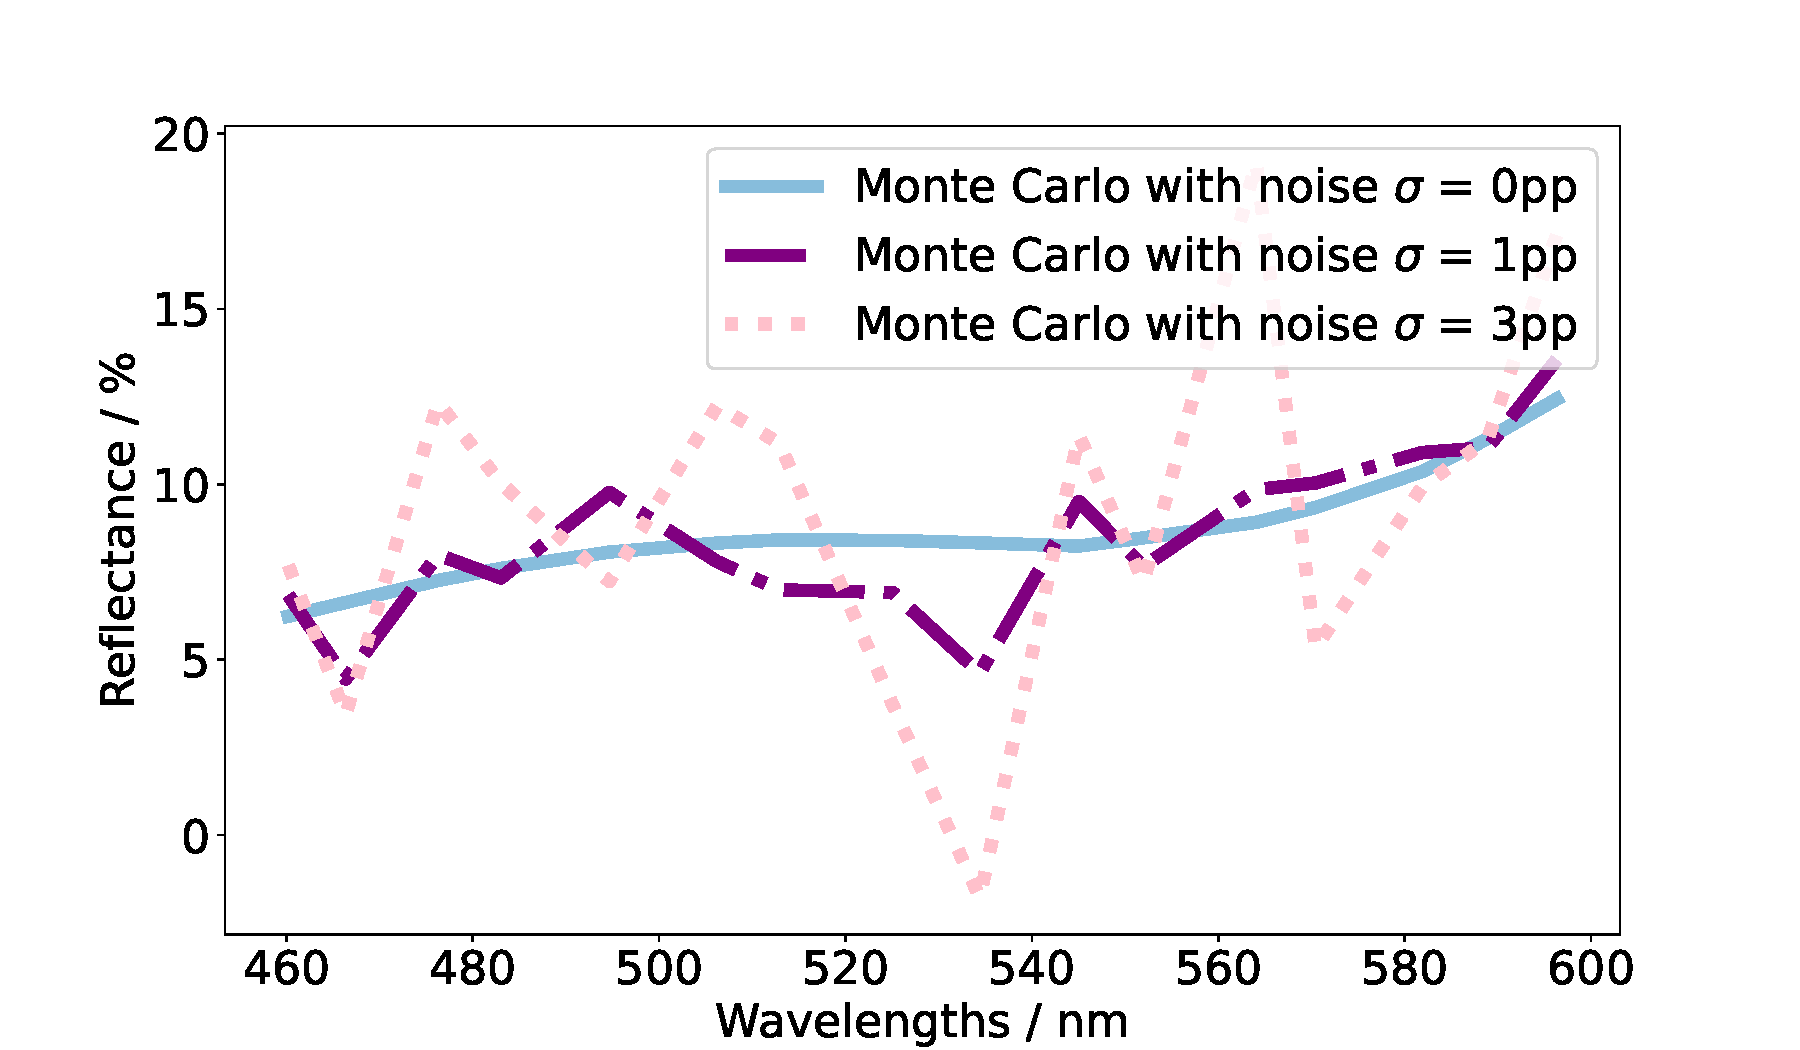
\includegraphics[width=\textwidth]{forwards_noise2_Q.pdf}
        \caption{}
        \label{fig:egforwards2noiseMCQ}
    \end{subfigure}
    \begin{subfigure}{0.49\textwidth}
        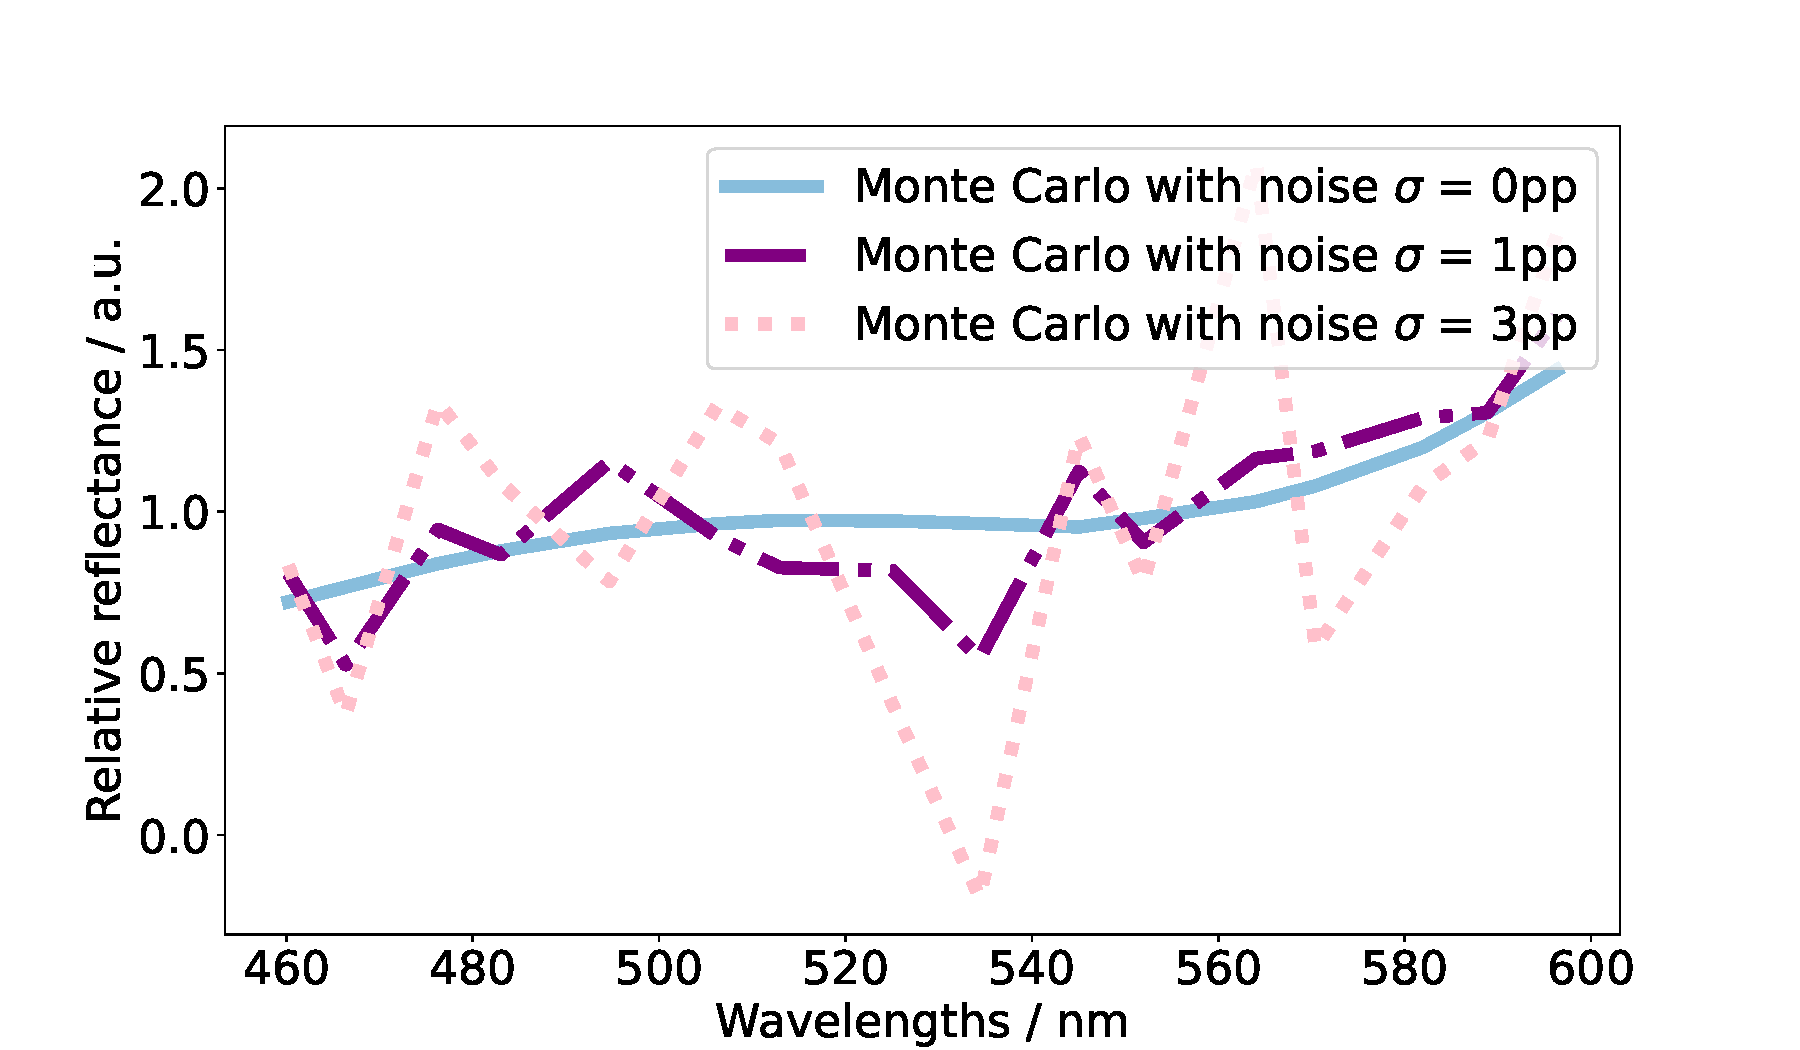
\includegraphics[width=\textwidth]{forwards_noise2_R.pdf}
        \caption{}
        \label{fig:egforwards2noiseMCR}
    \end{subfigure}
    \caption{Examples of the simulated camera response spectra from a single layer (top) or double layer (bottom) Monte Carlo simulated spectrum with noise levels of \textcolor{MyBlue}{0pp (solid)}, \textcolor{purple}{1pp (dash-dotted)}, and \textcolor{pink}{3pp (dotted)} for quantitative (left) and relative (right) data.}
    \label{fig:forwardsMCnoise}
\end{figure}

Each model is used to analyse the inverse problem of each of these varying noise level datasets and the evaluation of these results can be seen in Table \ref{tb:backwardsHSIMC} for $n=1.44$ (with further refractive indices in Appendices \ref{ap:backwardsHSIMCq} and \ref{ap:backwardsHSIMCr}) and examples of the $StO_2$ extraction quality in Figure \ref{fig:backwardsHSIMC1} for single-layer models and Figure \ref{fig:backwardsHSIMC2} for the double-layer model. Here $StO_2$ refers to the oxygenation of the single, homogeneous, semi-infinite layer for the single-layer models and the dermal oxygenation for the double-layer model. 

\begin{table}[h!]
    \centering
    \caption{The Pearson $r$ values (bold if $p<0.05$) of the linear regression line between the fitted tissue parameters and their ground truth displayed with their median absolute percentage errors ($APE$). This is shown for each variable when extracted by fitting Yudovsky 2009 single layer (Y1), Jacques 1999 (J), or Yudovsky 2009 double layer (Y2) to the quantitative (Q) or relative (R) Monte-Carlo datasets for $n=1.44$ at each noise level (0pp, 1pp, 3pp). All presented to 3s.f.}
    \begin{tabular}{|ccc|ccc|ccc|}
        \hline
        Parameter & Model & Quantitative & \multicolumn{3}{c}{$r$} & \multicolumn{3}{|c|}{median} \\
        & & (Q) or & \multicolumn{3}{c}{} & \multicolumn{3}{|c|}{$APE$ (\%)} \\
        & & Relative (R) & 0pp & 1pp & 3pp & 0pp & 1pp & 3pp \\
        \hline
        \multirow{6}{*}{$StO_2$} & \multirow{2}{*}{Y1} & Q & \textbf{0.999} & \textbf{0.825} & \textbf{0.369} & 1.90 & 24.8 & 85.2 \\
        & & R & \textbf{0.999} & \textbf{0.752} & \textbf{0.410} & 2.23 & 41.4 & 76.7 \\
        \cline{2-9}
        & \multirow{2}{*}{J} & Q & \textbf{0.978} & \textbf{0.829} & \textbf{0.402} & 4.06 & 22.5 & 83.6 \\
        & & R & \textbf{0.977} & \textbf{0.755} & \textbf{0.447} & 4.77 & 40.3 & 76.7 \\
        \cline{2-9}
        & \multirow{2}{*}{Y2} & Q & \textbf{0.751} & \textbf{0.302} & 0.142 & 16.8 & 56.1 & 68.9 \\
        & & R & \textbf{0.679} & 0.140 & 0.000746 & 18.8 & 68.2 & 73.3 \\
        \hline
        \multirow{6}{*}{$f_{blood}$} & \multirow{2}{*}{Y1} & Q & \textbf{0.984} & \textbf{0.667} & \textbf{0.450} & 5.83 & 23.7 & 51.8\\
        & & R & \textbf{0.870} & \textbf{0.547} & \textbf{0.535} & 16.7 & 47.5 & 51.1\\
        \cline{2-9}
        & \multirow{2}{*}{J} & Q & \textbf{0.924} & \textbf{0.719} & \textbf{0.498} & 7.14 & 25.0 & 46.7 \\
        & & R & \textbf{0.859} & \textbf{0.681} & \textbf{0.644} & 24.1 & 39.6 & 45.0 \\
        \cline{2-9}
        & \multirow{2}{*}{Y2} & Q & \textbf{0.872} & \textbf{0.389} & 0.147 & 23.1 & 88.3 & 131 \\
        & & R & \textbf{0.609} & \textbf{0.302} & 0.138 & 37.6 & 82.6 & 88.5 \\
        \hline
        \multirow{6}{*}{$a$} & \multirow{2}{*}{Y1} & Q & \textbf{0.992} & \textbf{0.773} & \textbf{0.558} & 3.85 & 18.7 & 35.1 \\
        & & R & \textbf{0.703} & 0.160 & \textbf{0.558} & 26.2 & 62.3 & 35.1 \\
        \cline{2-9}
        & \multirow{2}{*}{J} & Q & \textbf{0.961} & \textbf{0.759} & \textbf{0.542} & 4.69 & 17.1 & 30.4 \\
        & & R & \textbf{0.431} & -0.00356 & 0.166 & 27.7 & 57.7 & 51.7 \\
        \cline{2-9}
        & \multirow{2}{*}{Y2} & Q & \textbf{0.674} & 0.0572 & 0.0659 & 17.9 & 33.7 & 38.8 \\
        & & R & \textbf{0.333} & 0.054 & 0.0874 & 27.0 & 37.2 & 36.6 \\
        \hline
        \multirow{6}{*}{$b$} & \multirow{2}{*}{Y1} & Q & \textbf{0.998} & \textbf{0.751} & \textbf{0.516} & 2.63 & 21.8 & 52.0 \\
        & & R & \textbf{0.996} & \textbf{0.607} & \textbf{0.426} & 3.31 & 39.5 & 51.2 \\
        \cline{2-9}
        & \multirow{2}{*}{J} & Q & \textbf{0.934} & \textbf{0.757} & \textbf{0.515} & 5.70 & 23.7 & 50.4 \\
        & & R & \textbf{0.938} & \textbf{0.641} & \textbf{0.441} & 7.66 & 32.6 & 46.4 \\
        \cline{2-9}
        & \multirow{2}{*}{Y2} & Q & \textbf{0.735} & 0.117 & 0.0694 & 16.8 & 54.7 & 60.4 \\
        & & R & \textbf{0.360} & -0.0766 & 0.0794 & 33.2 & 64.3 & 55.8 \\
        \hline
        \multirow{2}{*}{$f_{mel}$} & \multirow{2}{*}{Y2} & Q & \textbf{0.852} & \textbf{0.546} & \textbf{0.538} & 28.0 & 98.6 & 107 \\ 
        & & R & \textbf{0.517} & \textbf{0.205} & 0.0613 & 35.3 & 159 & 152 \\
        \hline
        \multirow{2}{*}{$L_1$} & \multirow{2}{*}{Y2} & Q & \textbf{0.824} & \textbf{0.329} & \textbf{0.267} & 36.7 & 58.3 & 65.3 \\
        & & R & \textbf{0.806} & 0.00188 & -0.0188 & 38.1 & 72.8 & 71.6 \\
        \hline
    \end{tabular}    
    \label{tb:backwardsHSIMC}
\end{table}

%could reduce number of things shown below/put some in supplementary but unsure
\begin{figure}[h!]
    \centering
    \begin{subfigure}{0.49\textwidth}
        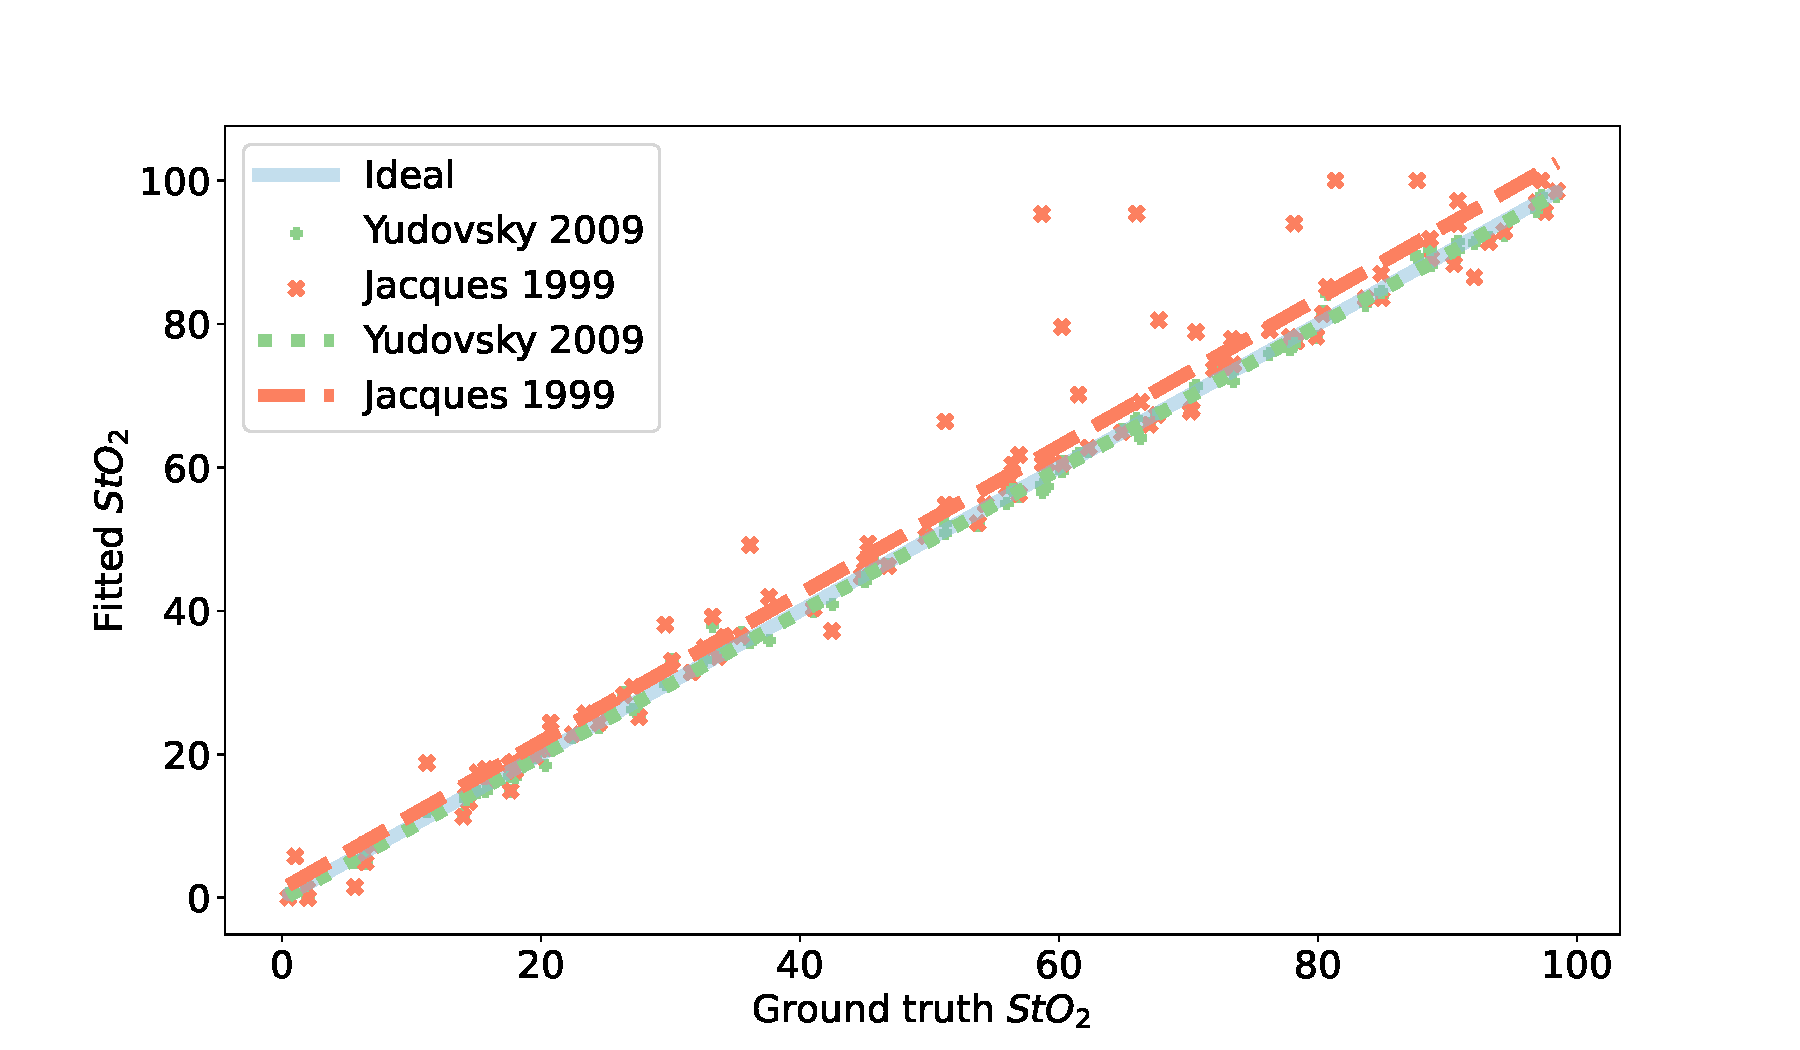
\includegraphics[width=\textwidth]{backwardsn0Q.pdf}
        \caption{}
        \label{fig:backwardsn0Q}
    \end{subfigure}
    \begin{subfigure}{0.49\textwidth}
        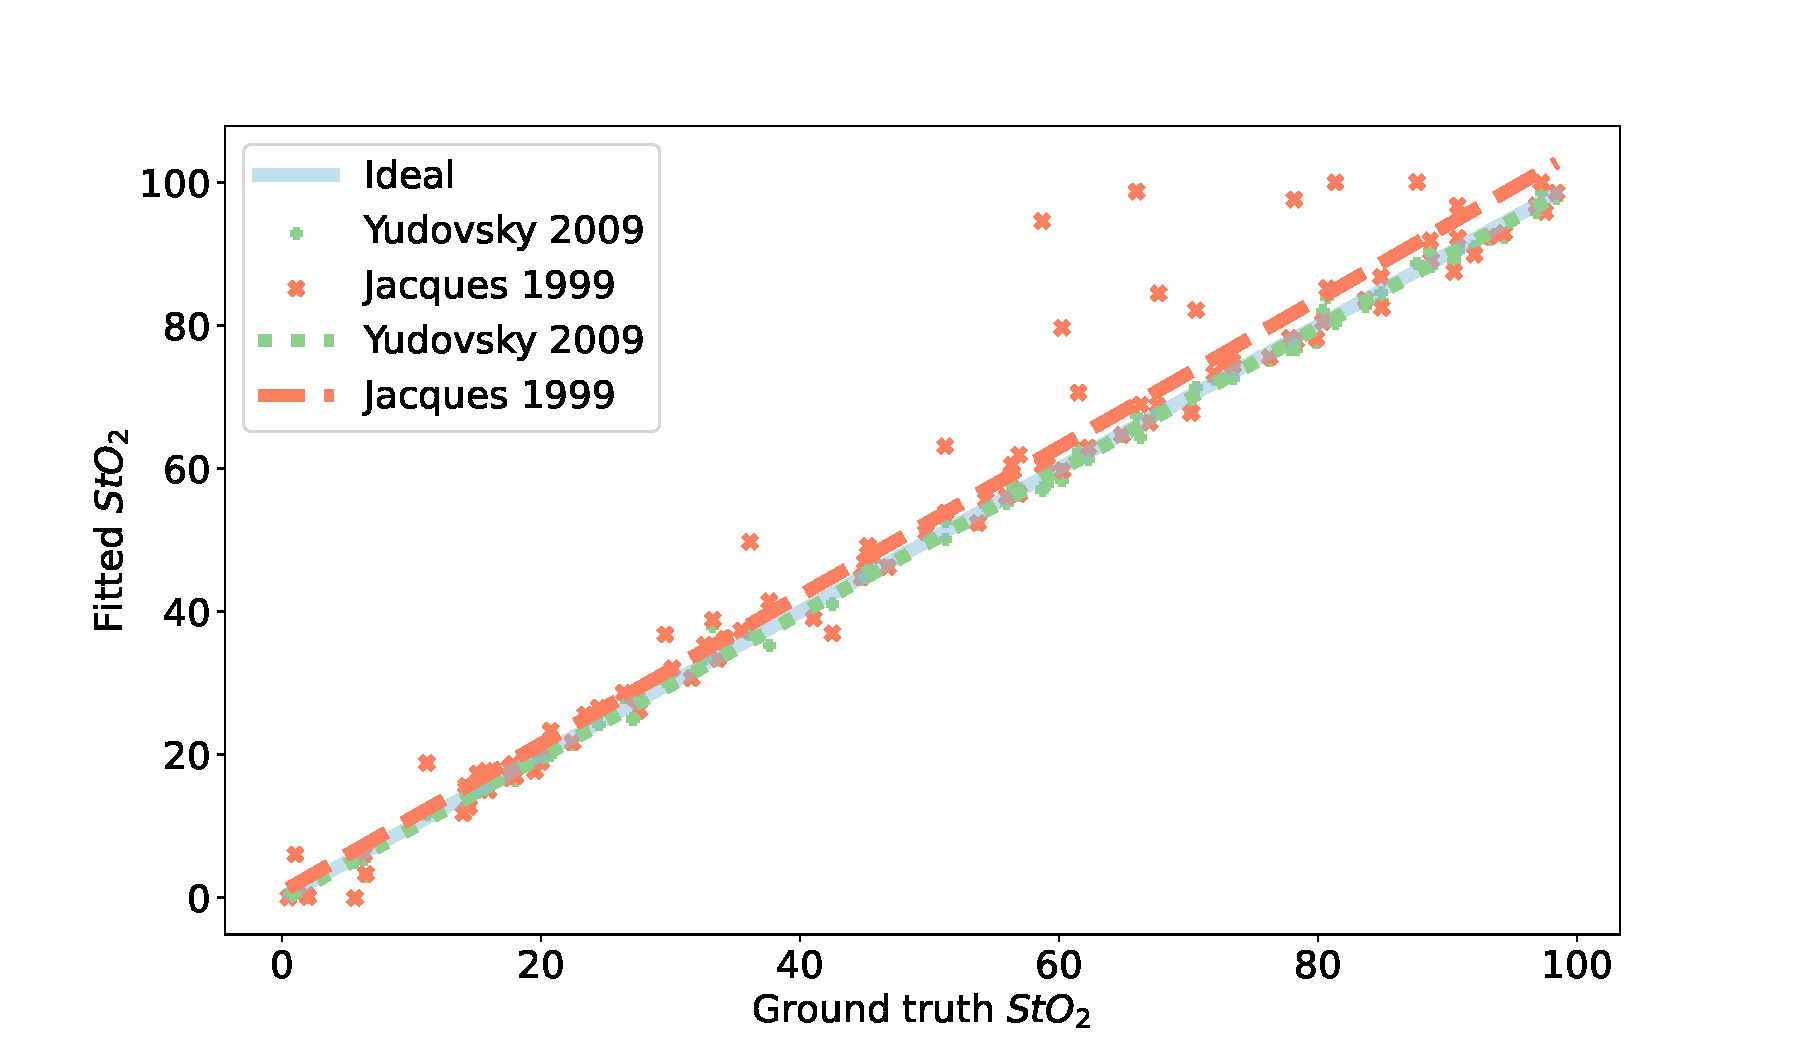
\includegraphics[width=\textwidth]{backwardsn0R.pdf}
        \caption{}
        \label{fig:backwardsn0R}
    \end{subfigure}
    \begin{subfigure}{0.49\textwidth}
        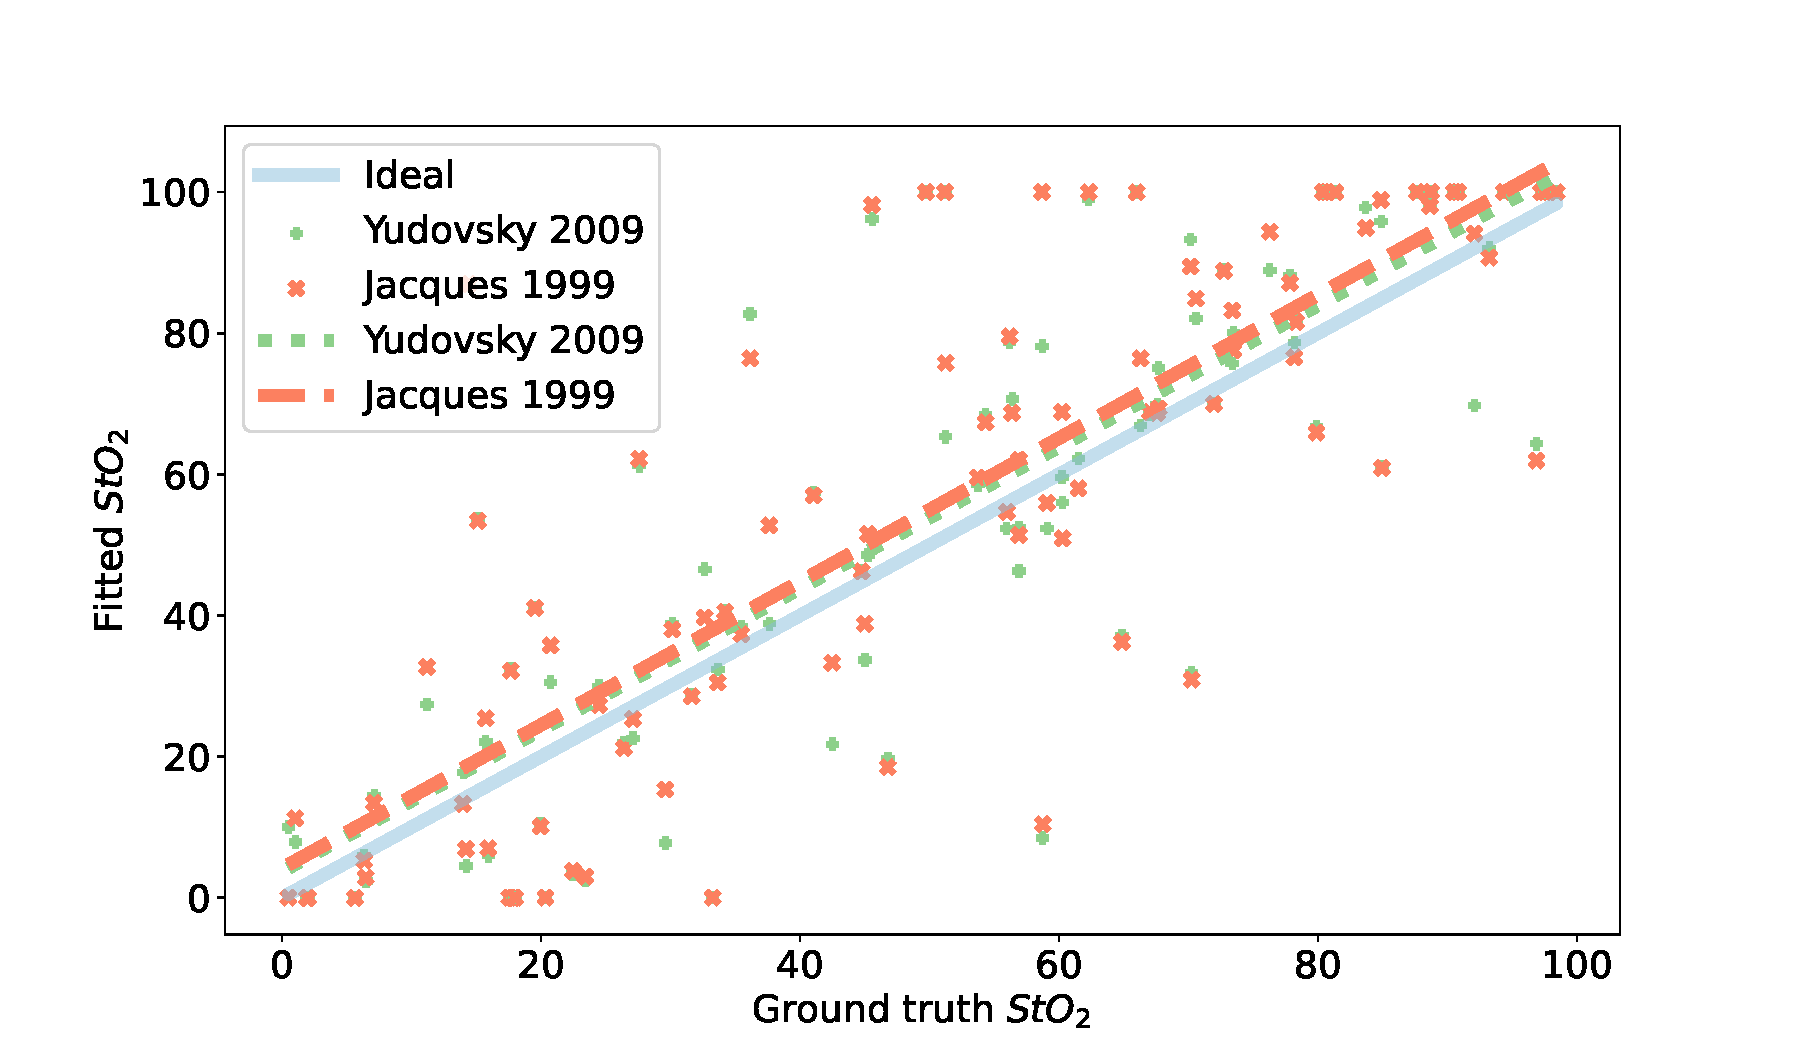
\includegraphics[width=\textwidth]{backwardsn0.01Q.pdf}
        \caption{}
        \label{fig:backwardsn0.01Q}
    \end{subfigure}
    \begin{subfigure}{0.49\textwidth}
        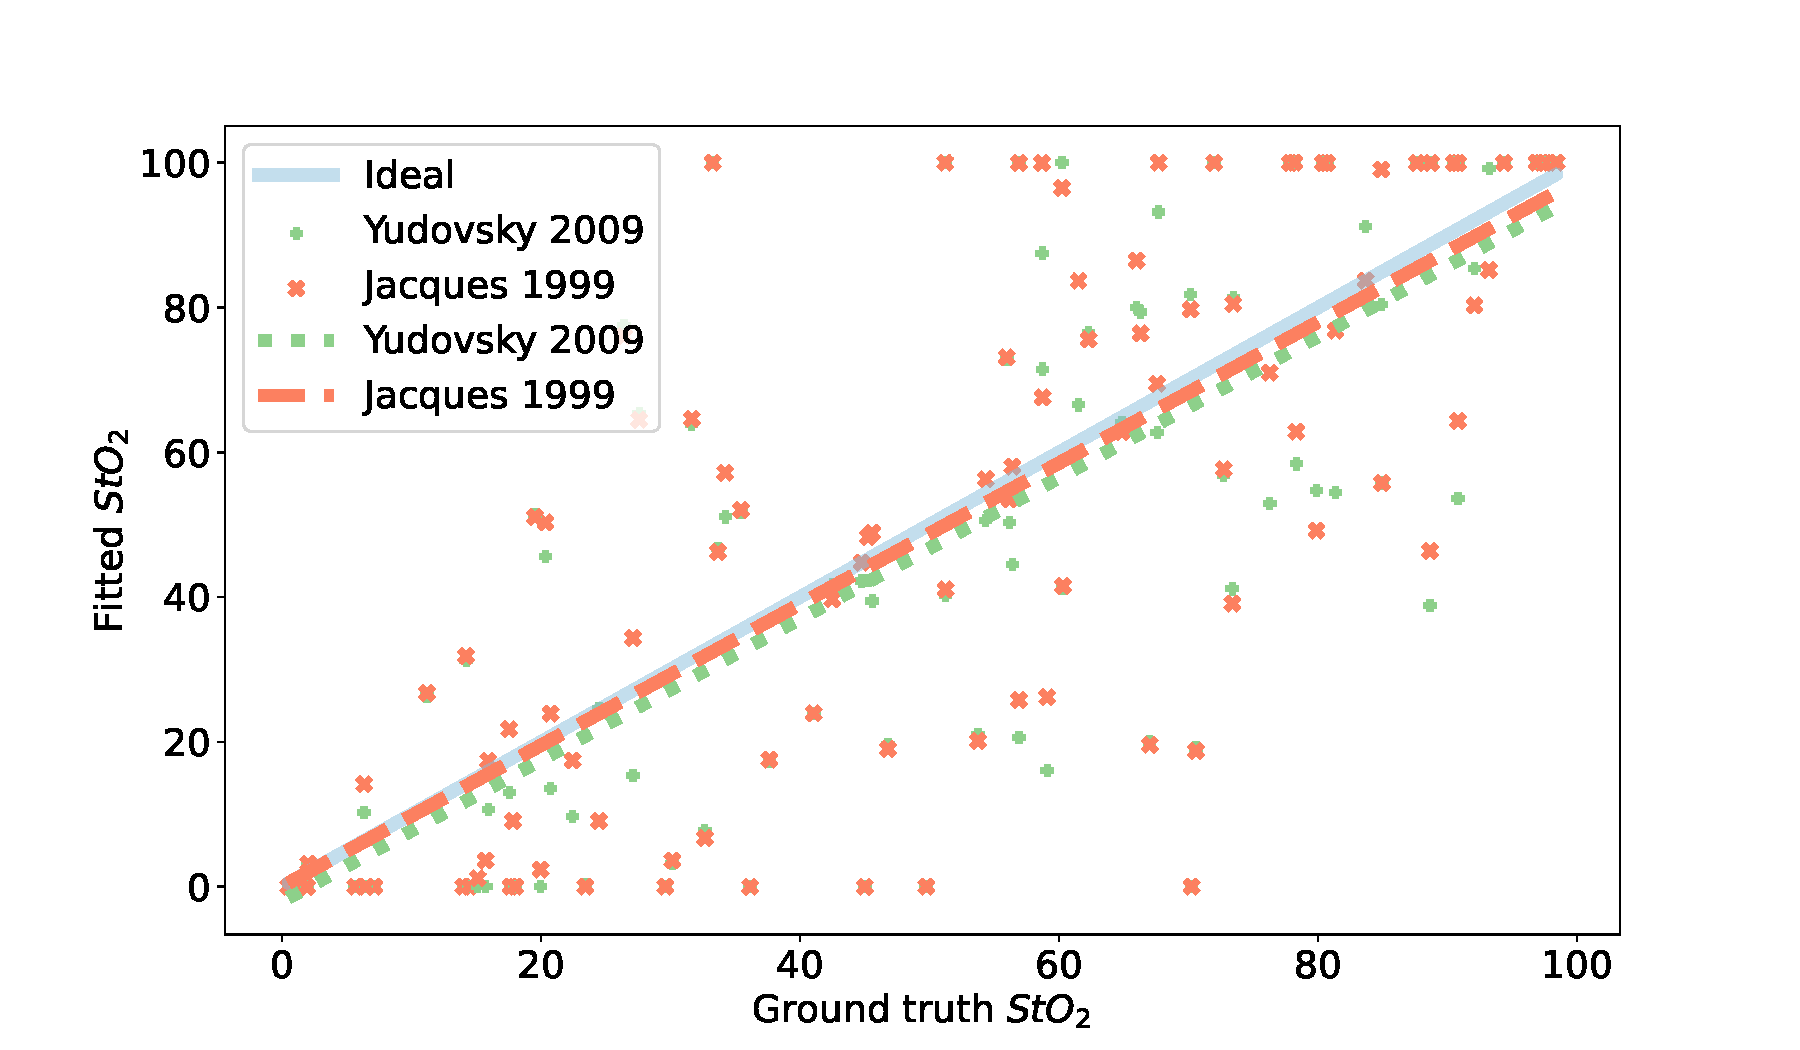
\includegraphics[width=\textwidth]{backwardsn0.01R.pdf}
        \caption{}
        \label{fig:backwardsm0.01R}
    \end{subfigure}
    \begin{subfigure}{0.49\textwidth}
        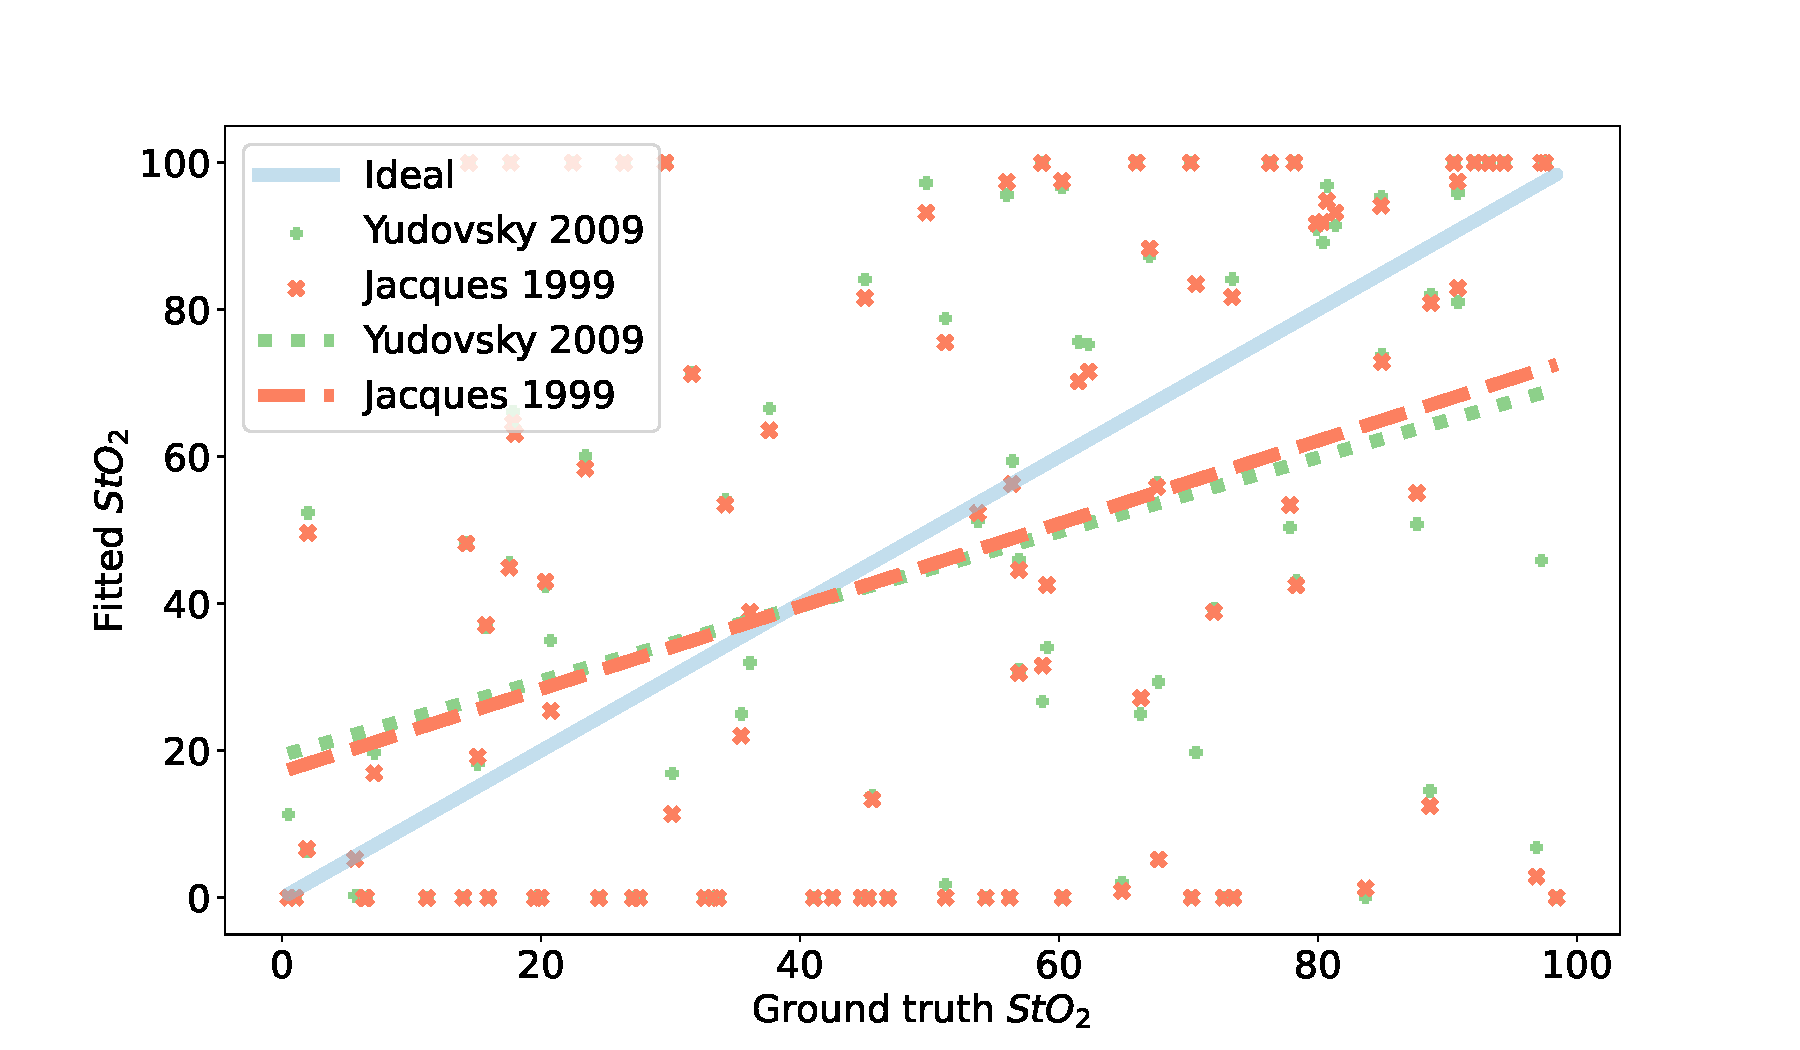
\includegraphics[width=\textwidth]{backwardsn0.03Q.pdf}
        \caption{}
        \label{fig:backwardsn0.03Q}
    \end{subfigure}
    \begin{subfigure}{0.49\textwidth}
        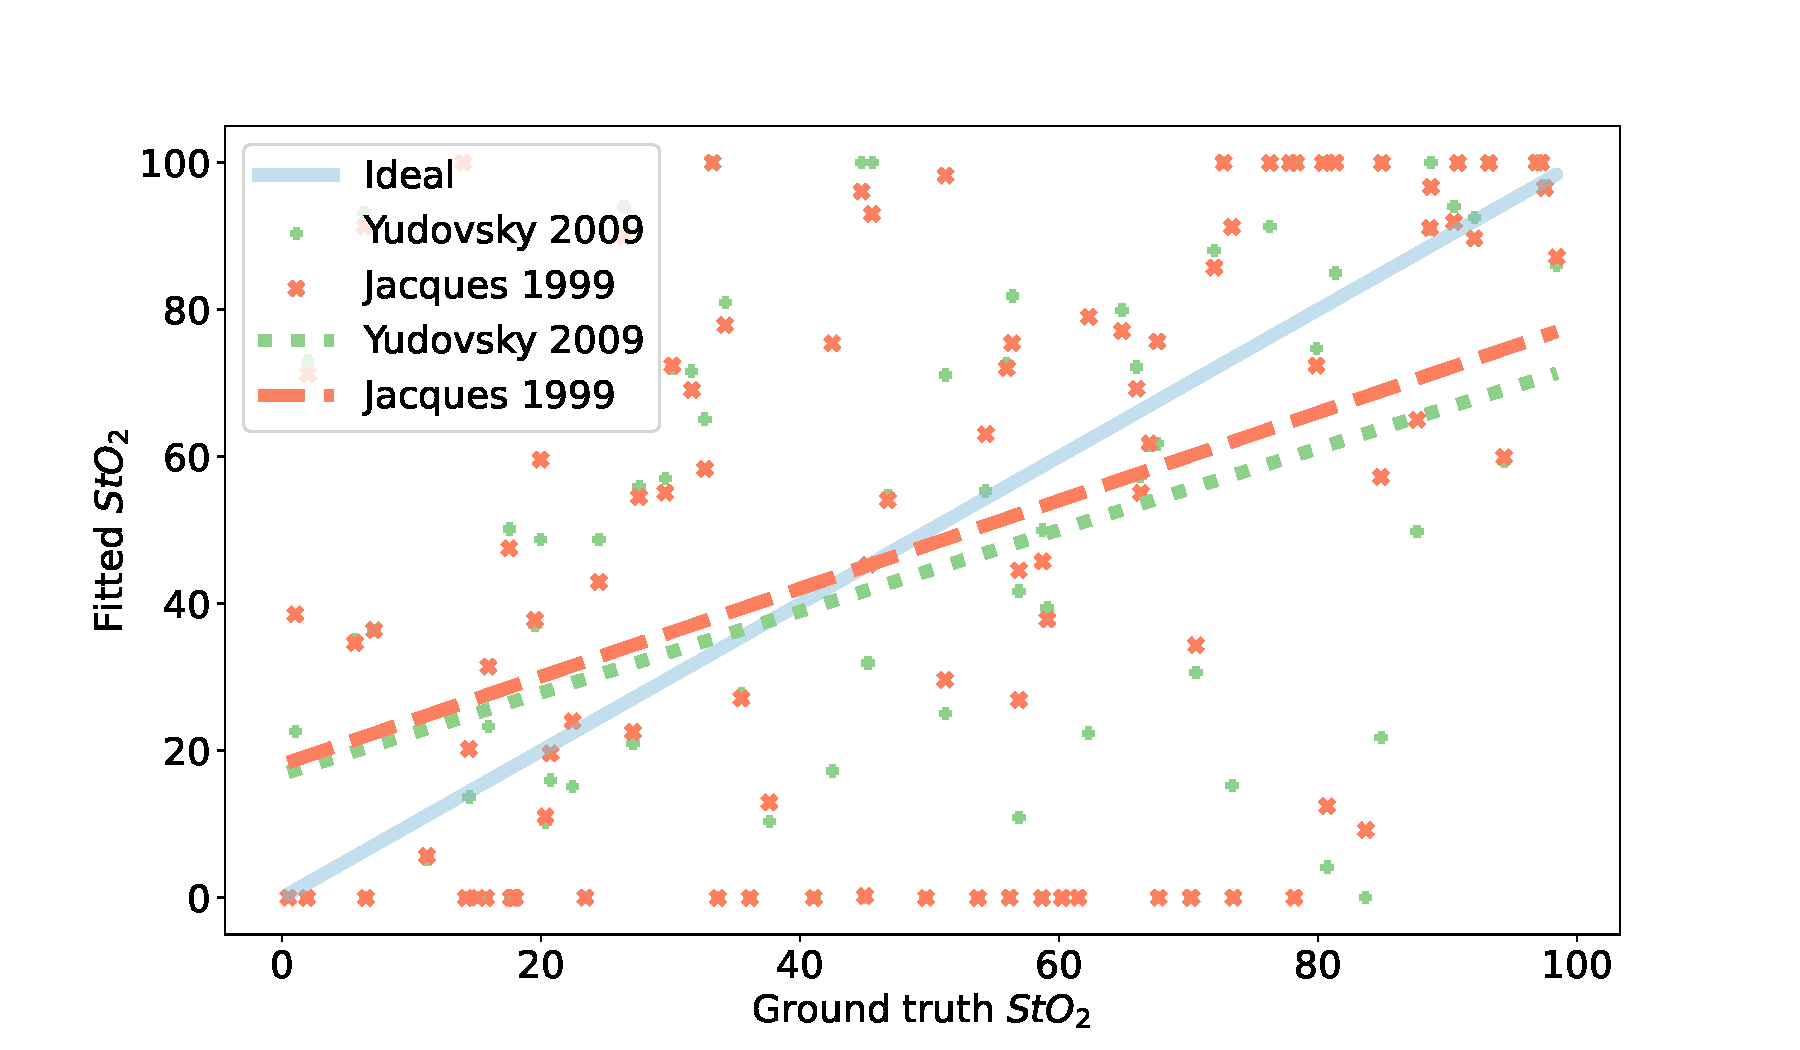
\includegraphics[width=\textwidth]{backwardsn0.03R.pdf}
        \caption{}
        \label{fig:backwardsm0.03R}
    \end{subfigure}
    \caption{An example of the quality of parameter recovery by fitting each inverse analytical model (Yudovsky 2009 (\textcolor{MyGreen}{green $+$}) and Jacques 1999 (\textcolor{MyOrange}{orange $\times$})) to the quantitative (left) or relative (right) simulated camera responses from the Monte Carlo simulations and their associated trend lines for a refractive index of 1.44 for $StO_2$. This is shown for data with either no added noise (top) or added noise with $\sigma = 1pp$ (middle) or $\sigma = 3pp$ (bottom).}
    \label{fig:backwardsHSIMC1}
\end{figure}

\begin{figure}[h!]
    \centering
    \begin{subfigure}{0.49\textwidth}
        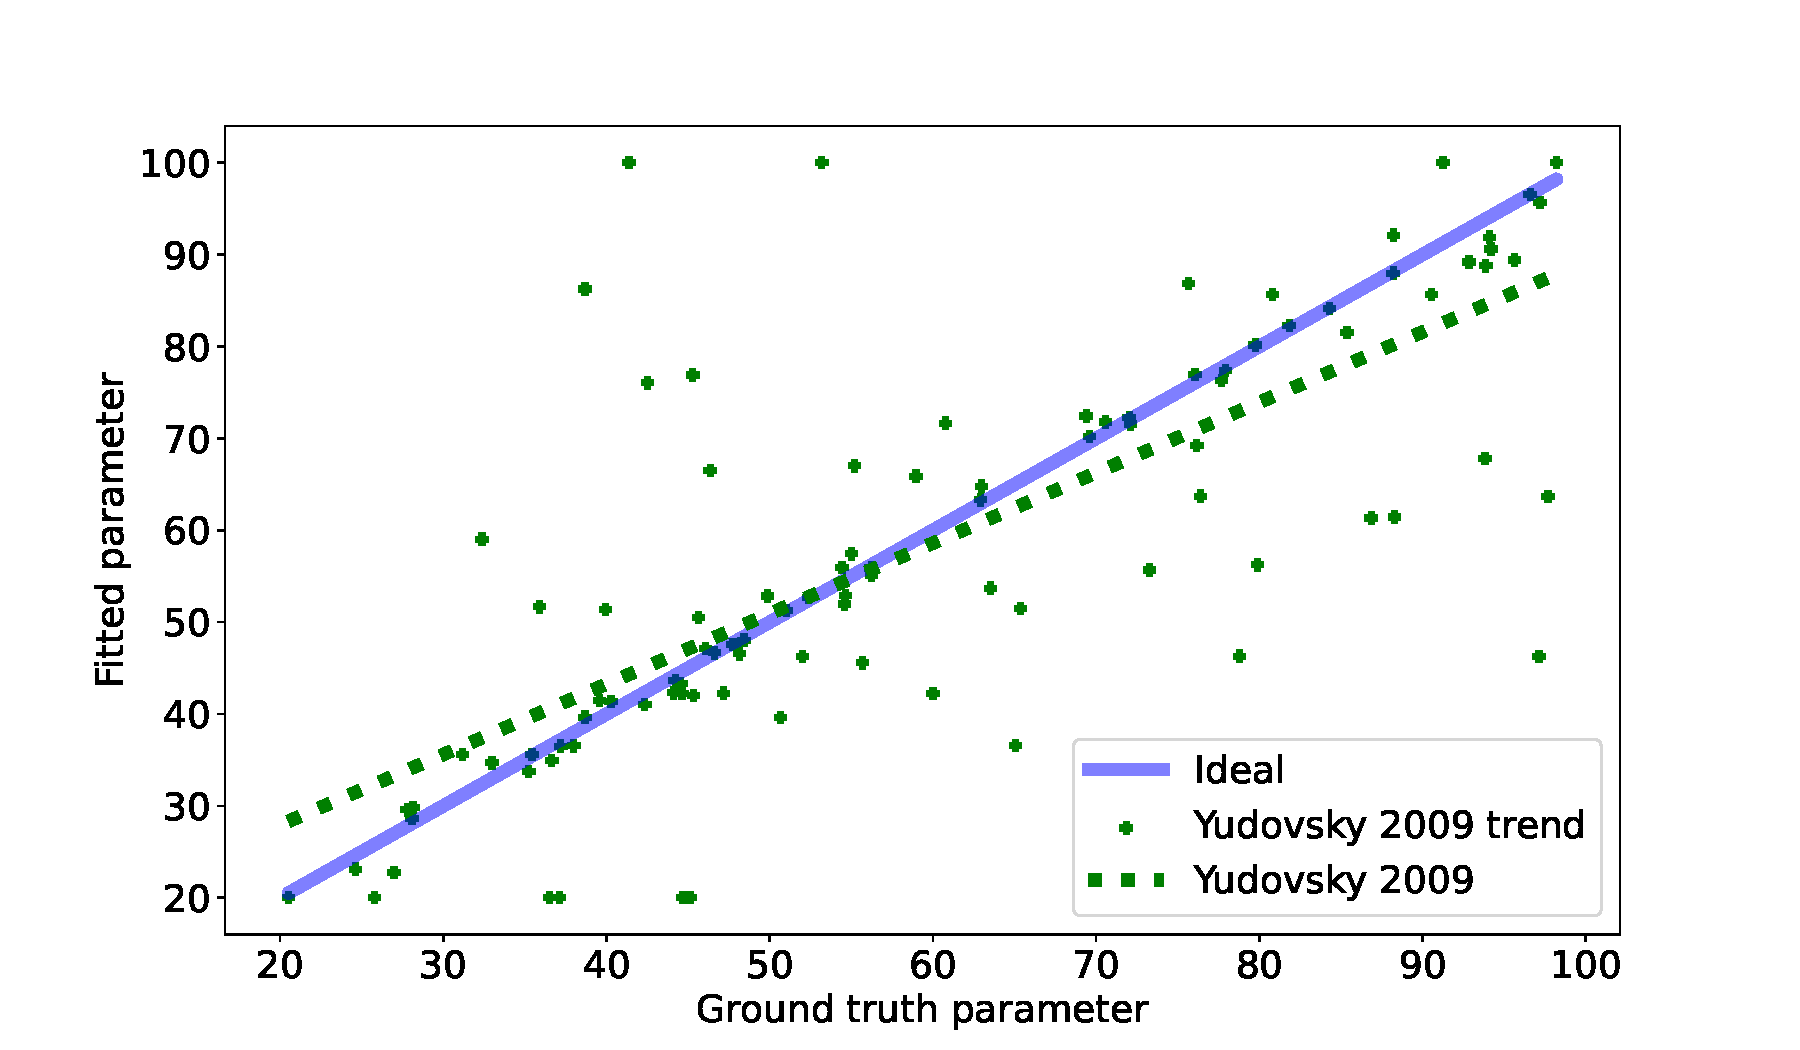
\includegraphics[width=\textwidth]{backwardsn0Q2.pdf}
        \caption{}
        \label{fig:backwardsn0Q2}
    \end{subfigure}
    \begin{subfigure}{0.49\textwidth}
        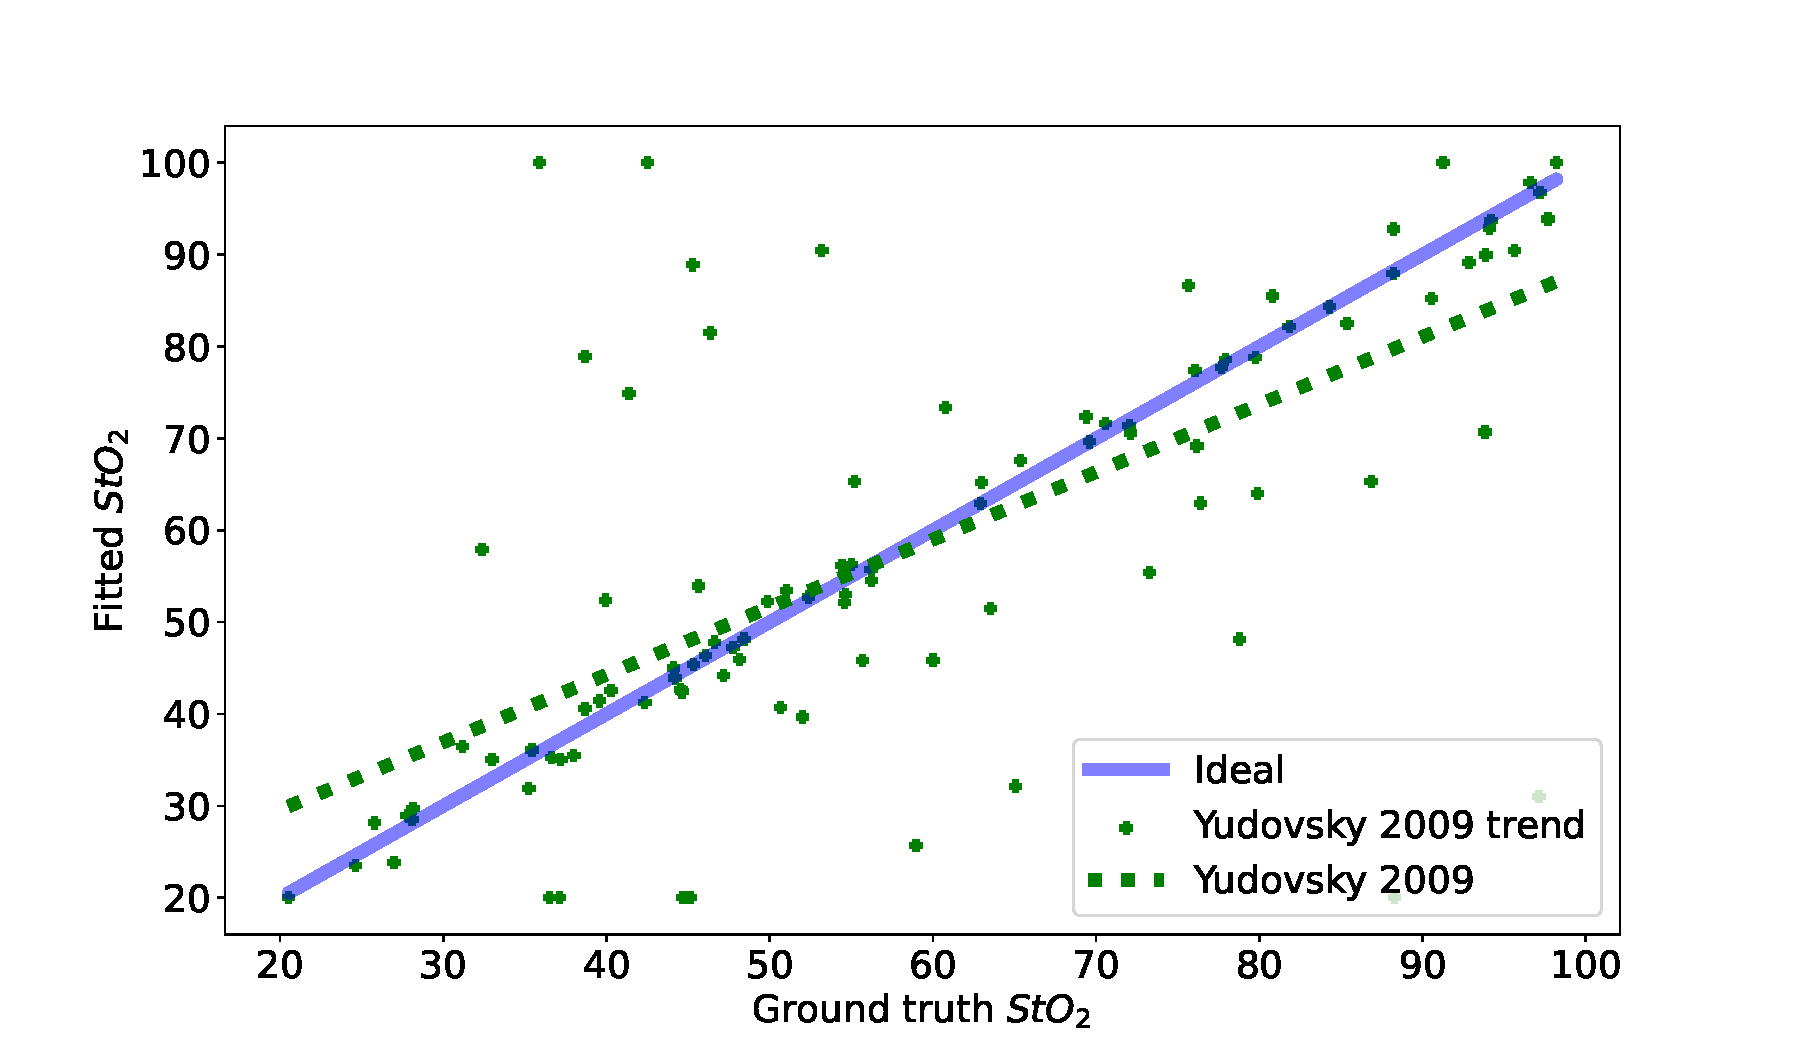
\includegraphics[width=\textwidth]{backwardsn0R2.pdf}
        \caption{}
        \label{fig:backwardsn0R2}
    \end{subfigure}
    \begin{subfigure}{0.49\textwidth}
        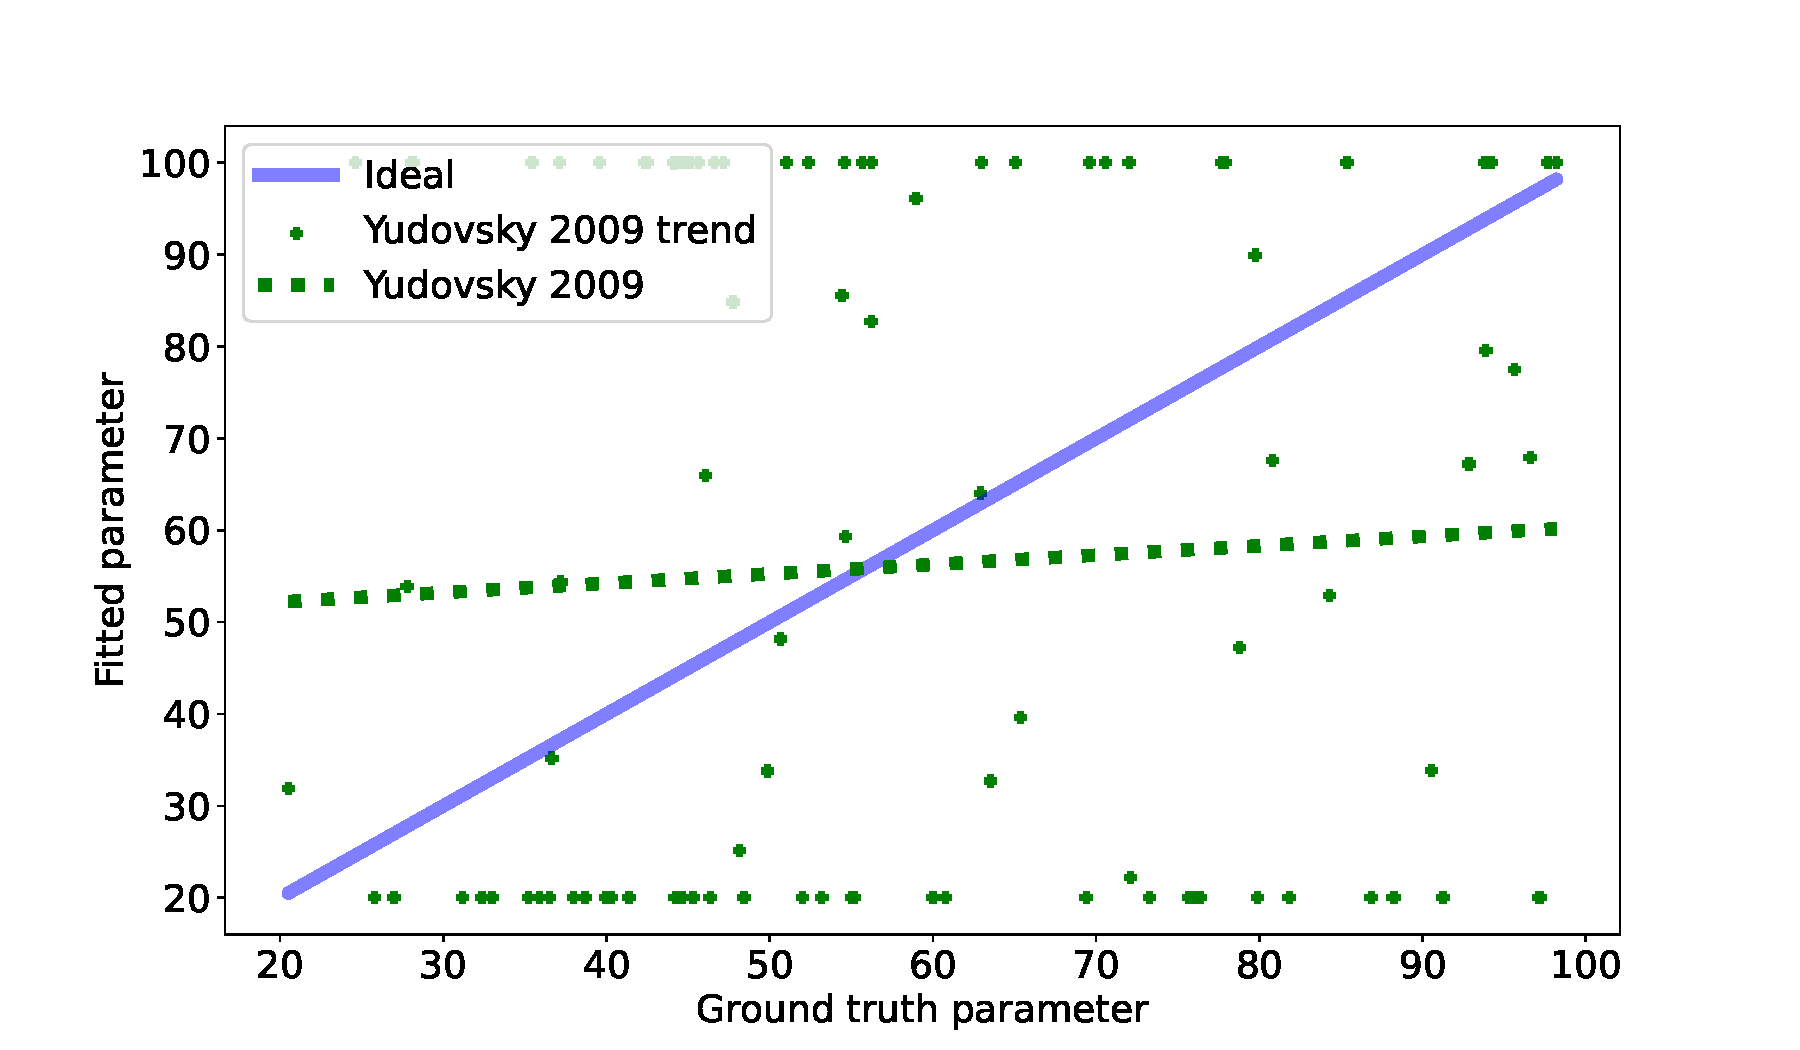
\includegraphics[width=\textwidth]{backwardsn0.01Q2.pdf}
        \caption{}
        \label{fig:backwardsn0.01Q2}
    \end{subfigure}
    \begin{subfigure}{0.49\textwidth}
        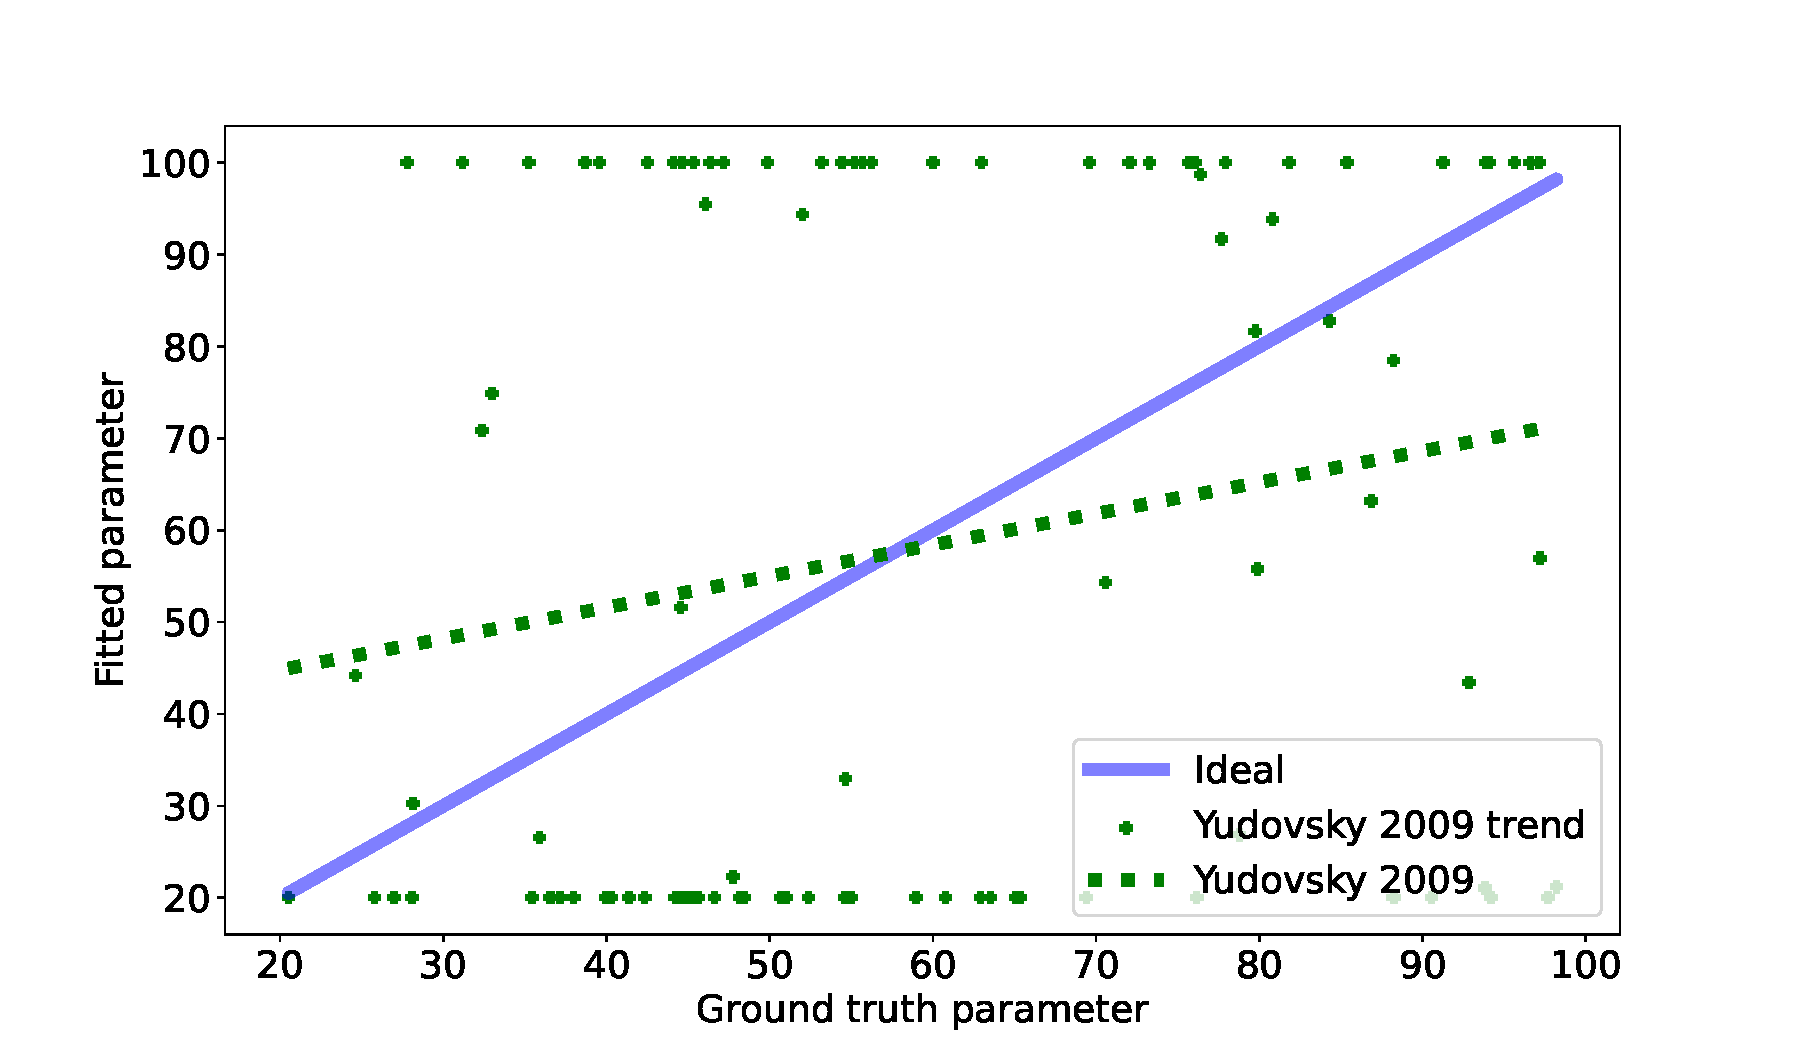
\includegraphics[width=\textwidth]{backwardsn0.01R2.pdf}
        \caption{}
        \label{fig:backwardsm0.01R2}
    \end{subfigure}
    \begin{subfigure}{0.49\textwidth}
        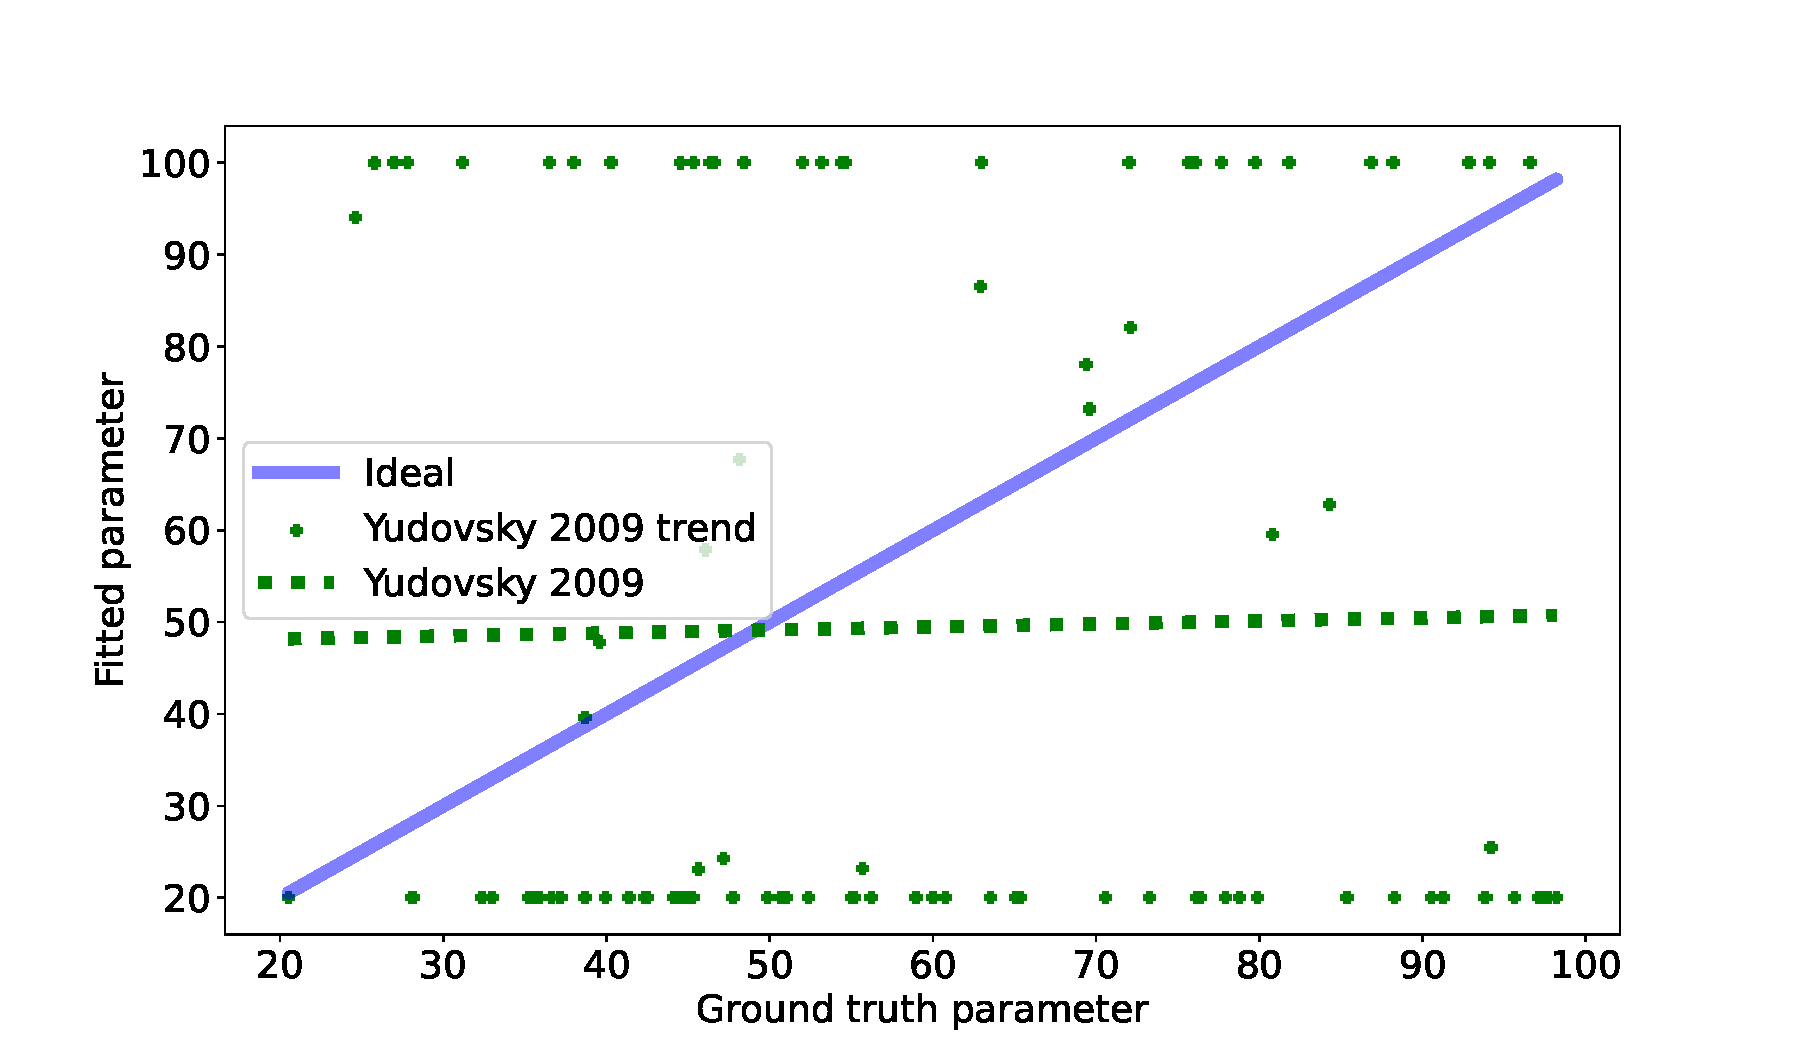
\includegraphics[width=\textwidth]{backwardsn0.03Q2.pdf}
        \caption{}
        \label{fig:backwardsn0.03Q2}
    \end{subfigure}
    \begin{subfigure}{0.49\textwidth}
        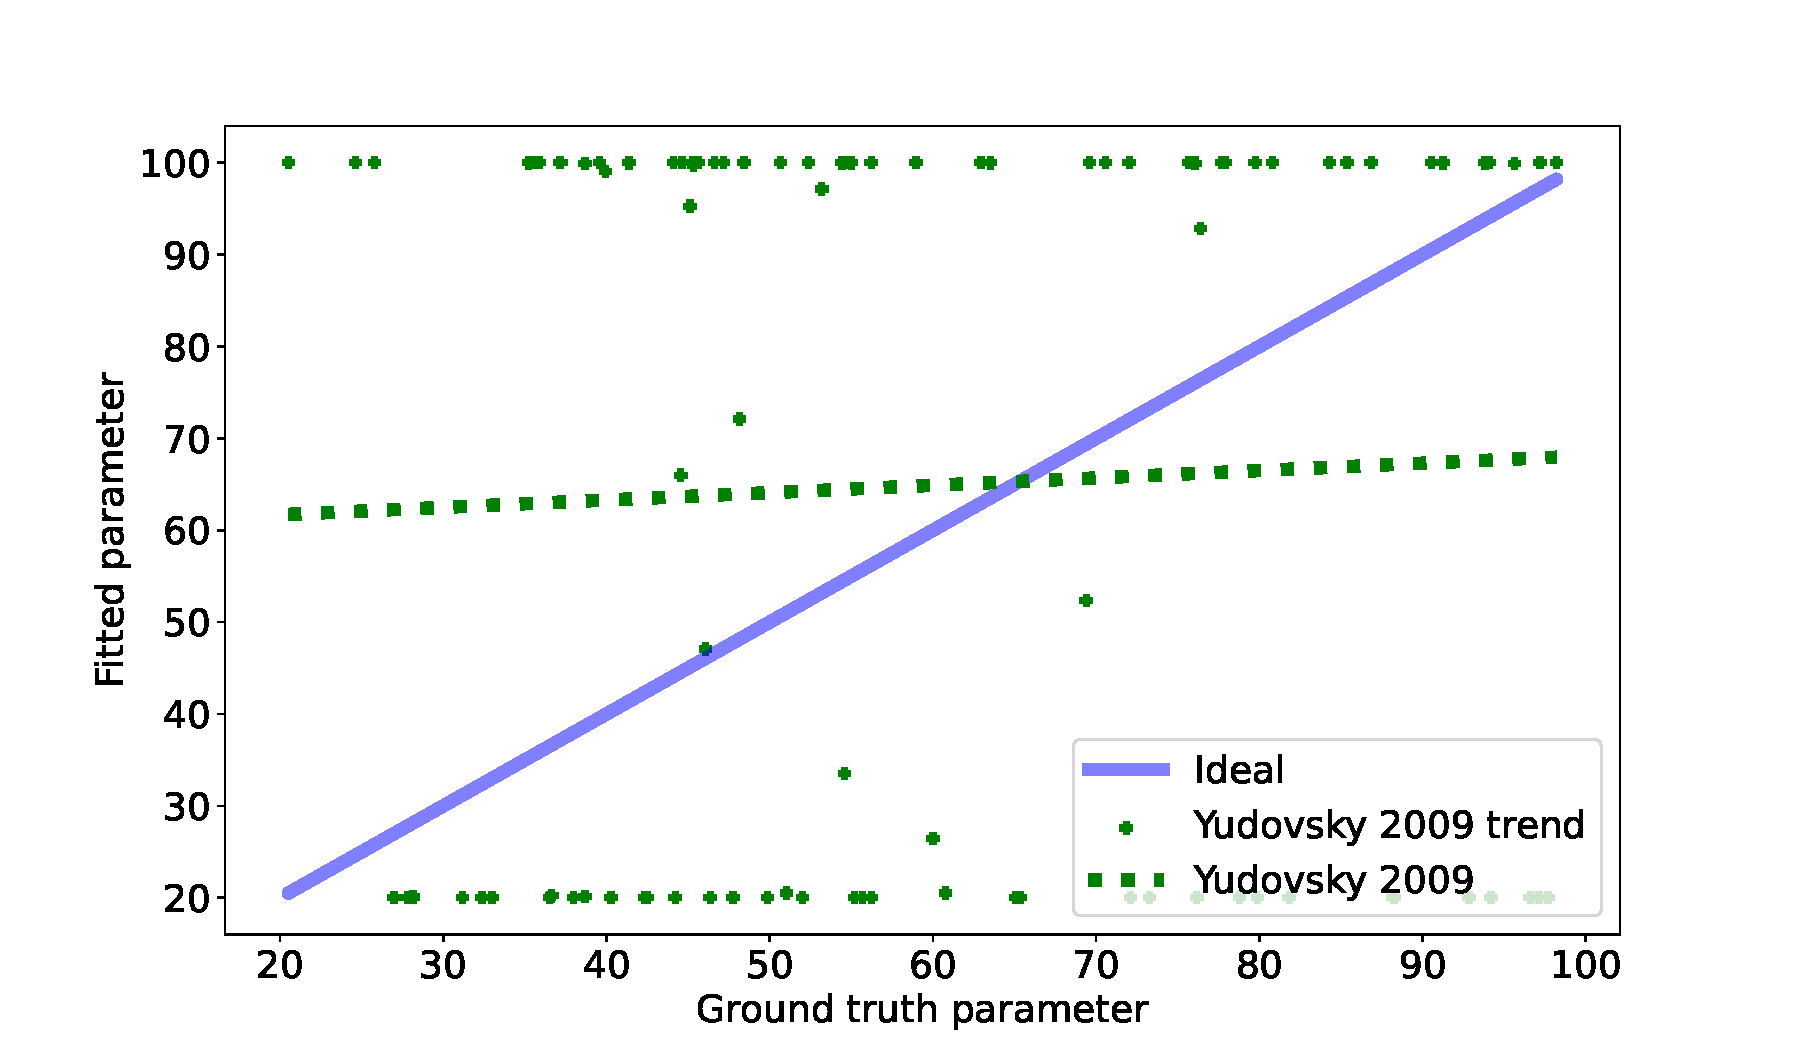
\includegraphics[width=\textwidth]{backwardsn0.03R2.pdf}
        \caption{}
        \label{fig:backwardsm0.03R2}
    \end{subfigure}
    \caption{An example of the quality of parameter recovery by fitting the double-layer inverse analytical model Yudovsky 2009 (\textcolor{MyGreen}{green $+$}) to the quantitative (left) or relative (right) simulated camera responses from the Monte Carlo simulations and their associated trend lines for a refractive index of 1.44 for $StO_2$. This is shown for data with either no added noise (top) or added noise with $\sigma = 1pp$ (middle) or $\sigma = 3pp$ (bottom).}
    \label{fig:backwardsHSIMC2}
\end{figure}
\FloatBarrier

\subsection{Gelatin-based tissue phantoms}
To evaluate the quality of camera response simulation, the mean spectrum from the annotated region of each HSI image of a phantom is compared to the camera response simulation generated from the spectrophotometer diffuse reflectance measurement of these phantoms and the forwards models using ground truth parameters in Table \ref{tb:forwardsHSIphantoms} and an example seen in Figure \ref{fig:forwardsHSIphantoms}. 

\begin{table}[h!] %could remove noise levels here
    \centering
    \caption{Mean (standard deviation) $NRMSE$ (3.d.p.) between the simulated camera responses of each forwards spectrum from the Yudovsky 2009 single-layer model (Y1), the Jacques 1999 model (J), or using spectrophotometer measurements of each phantom (S) and each mean spectrum from an annotated HSI image of each phantom using the same ground truth variable parameters for quantitative and relative data. This is presented with the Pearson $r$ (bold if Pearson $p < 0.05$) for the linear regression between all forwards spectra against mean HSI phantom spectra for each analytical model or spectrophotometer measurements. All metrics are evaluated for the wavelength region of 450-575nm.}
    \begin{tabular}{|c|c|cc|}
        \hline
        Model & Quantitative (Q) & $NRMSE$ & $r$ \\
         & or Relative (R) &  & \\
        \hline
        \multirow{2}{*}{Y1} & Q & 0.209 (0.177) & \textbf{0.994} \\
        & R & 0.055 (0.032) & \textbf{0.986} \\ %stats are slightly better if flatfield balance then normalise but using specsens for thesis storyline 
        \hline
        \multirow{2}{*}{J} & Q & 0.204 (0.196) & \textbf{0.994} \\
        & R & 0.061 (0.042) & \textbf{0.981} \\
        \hline
        \multirow{2}{*}{S} & Q & 0.276 (0.182) & \textbf{0.996} \\
         & R & 0.054 (0.030) & \textbf{0.986} \\
        \hline
    \end{tabular}
    \label{tb:forwardsHSIphantoms}
\end{table}

\begin{figure}[h!]
    \centering
    \begin{subfigure}{0.49\textwidth}
        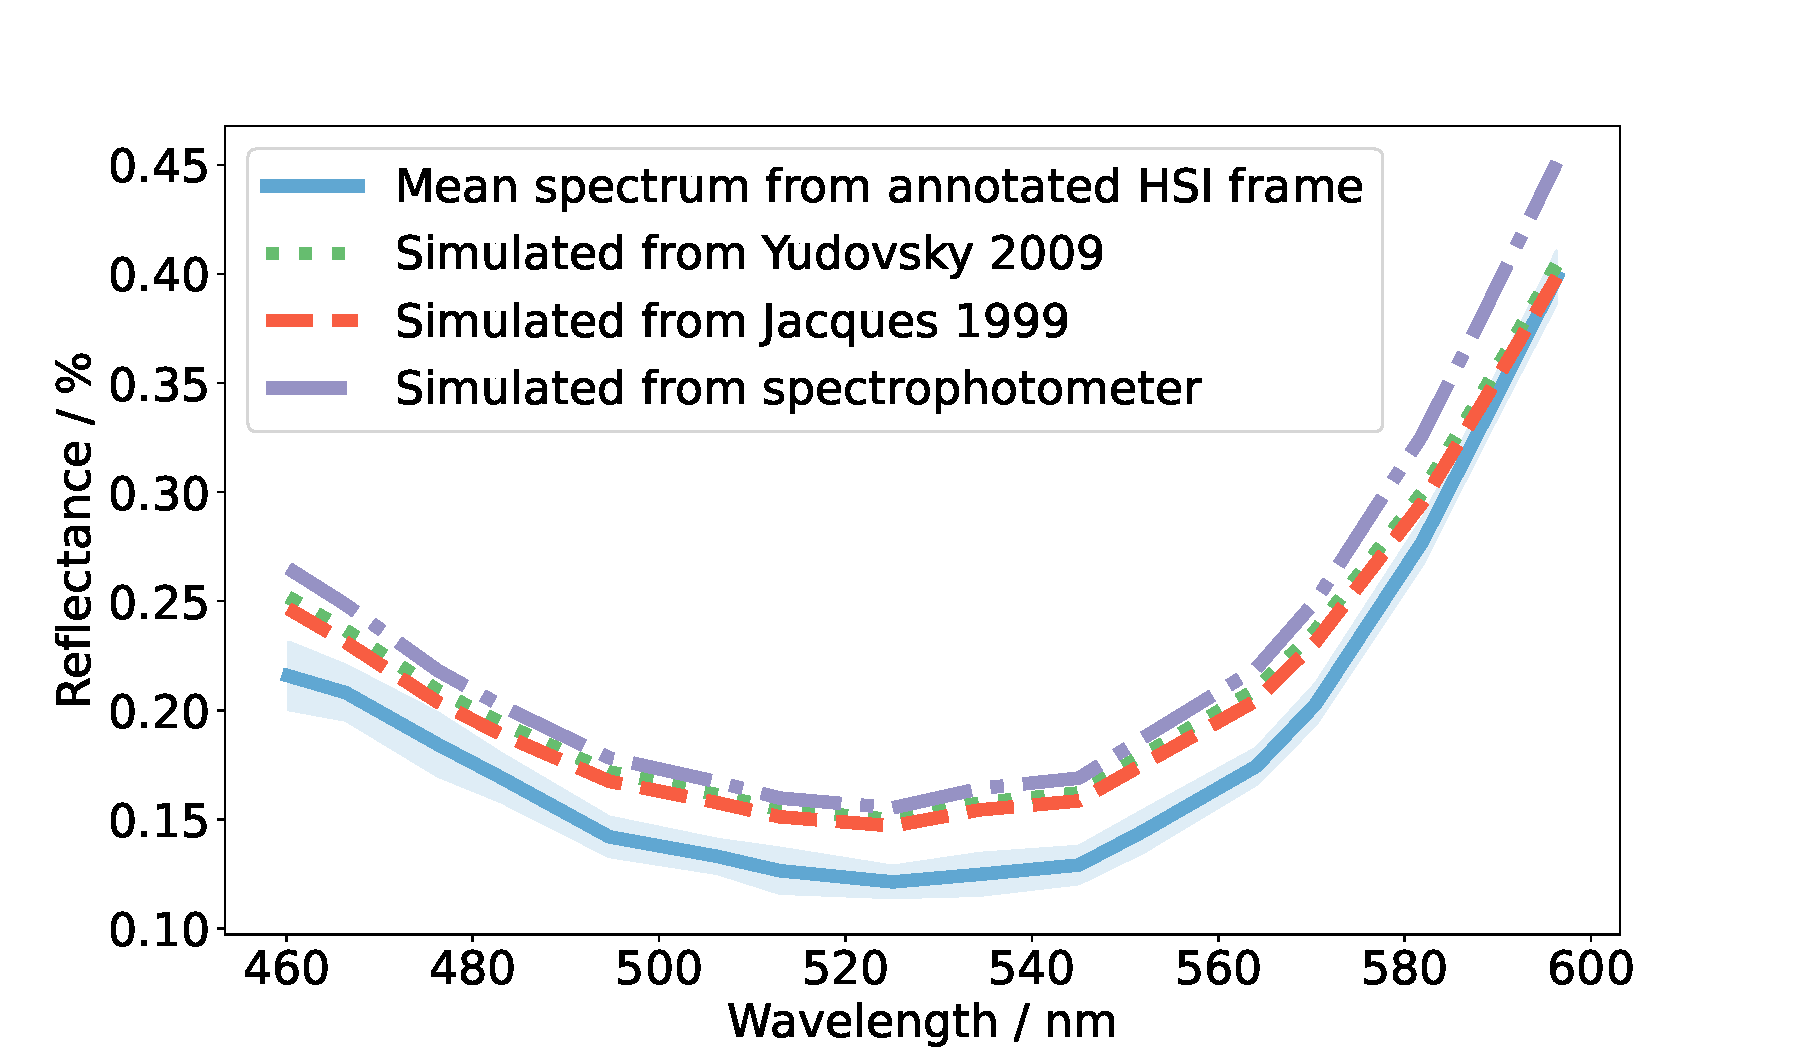
\includegraphics[width=\textwidth]{forwardsHSIphantomQ.pdf}
        \caption{}
        \label{fig:egforwardsHSIQ}
    \end{subfigure}
    \begin{subfigure}{0.49\textwidth}
        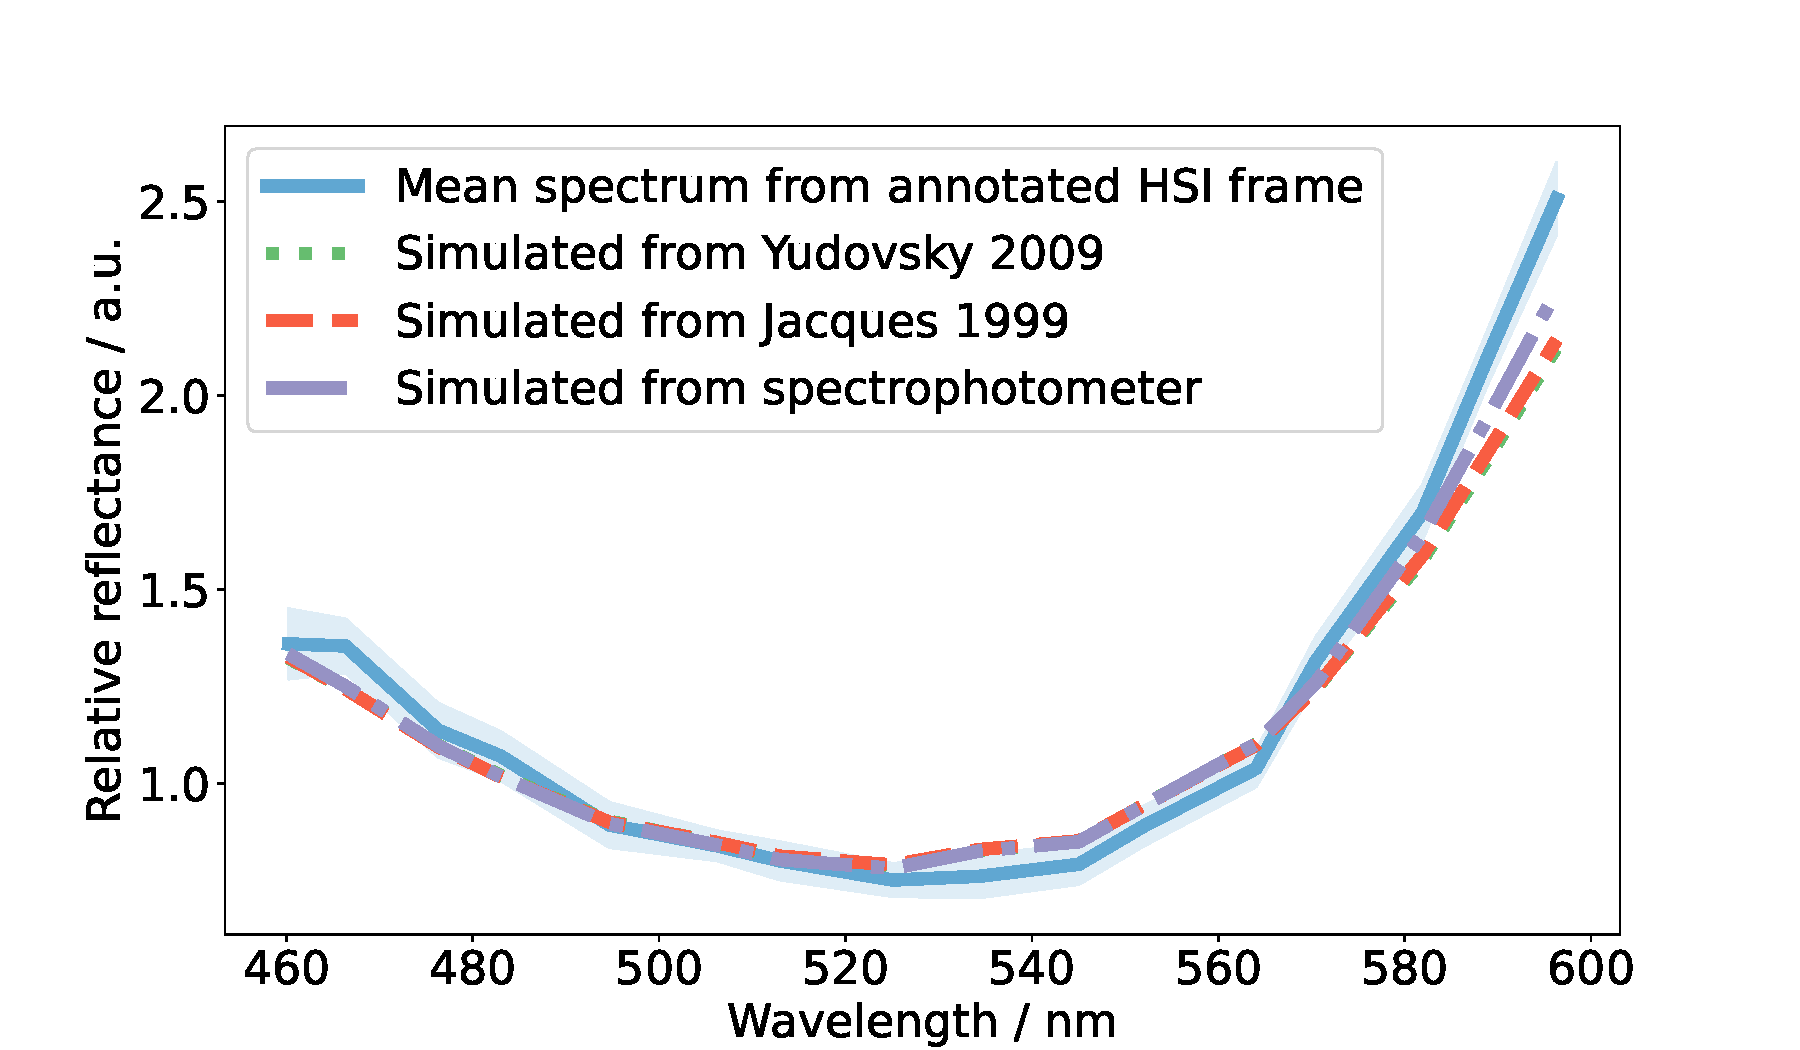
\includegraphics[width=\textwidth]{forwardsHSIphantomR.pdf}
        \caption{}
        \label{fig:egforwardsHSIR}
    \end{subfigure}
    \caption{Example of the simulated camera response spectra from each forward single-layer analytical model: Yudovsky 2009 (\textcolor{MyGreen}{green dotted}) and Jacques 1999 (\textcolor{MyOrange}{orange dashed}), using ground truth variables for a refractive index of 1.44 compared to that predicted using spectrophotometer measurements (\textcolor{purple}{purple dash-dotted} and the mean spectrum from an HSI image of the same phantom (\textcolor{MyBlue}{blue solid}) for quantitative (left) and relative (right) data.}
    \label{fig:forwardsHSIphantoms}
\end{figure}

Each single-layer model is also fitted to the mean spectrum of each annotated image, with results shown in Table \ref{tb:backwardsHSIphantomsann} and examples of $AR1$ parameter extraction shown in Figure \ref{fig:backwardsHSIphantomsann}. A similar analysis is performed on a pixelwise basis on annotated regions of each phantom using either a single frame or the mean of 5 frames of the hyperspectral video. The results of this can also be seen in Table \ref{tb:backwardsHSIphantomsann} and Figure \ref{fig:backwardsHSIphantomsann}.
%Since Yudovsky 2009 has shown to perform better than Jacques 1999 in both Chapter \ref{chap:1layer} and this chapter, the inverse of this model is tested on a pixel-by-pixel basis. % on relative data for comparison with the performance on neurosurgical HSI data. 
An example sRGB reconstruction with the annotated region shown alongside the pixel-by-pixel $AR1$ recovery and the pixel-by-pixel $APE$ is shown in Figure \ref{fig:gelatinpbpeg} using Yudovsky 2009 on relative data from a single frame, and \ref{fig:gelatinpbpeg5} when fitted to relative data from the mean of 5 frames. The mean annotated spectrum ($\pm$ standard deviation) for each case is also presented alongside the modelled spectrum using ground-truth parameters and parameters fitted to the mean annotated spectrum in Figure \ref{fig:gelatinpbpeg}. Similar figures can be found fitting to quantitative data or using the Jacques 1999 model in Appendices \ref{ap:MoreHSIPhantomEgs}.

\begin{table}[h!]
    \centering
    \caption{The Pearson $r$ values (bold if $p<0.05$) of the linear regression line between the fitted phantom parameters and their ground truth displayed with their median absolute percentage errors ($APE$). This is shown for each variable when extracted by fitting Yudovsky 2009 single layer (Y) or Jacques 1999 (J) to each quantitative (Q) or relative (R) mean annotated spectra or pixel-by-pixel in the annotated regions of data from 1 frame or the mean of 5 frames of each hyperspectral video from the HSI phantom dataset using $n=1.35$. All presented to 3s.f.}
    \begin{tabular}{|ccc|cc|cc|cc|}
        \hline
       \multirow{3}{*}{Parameter} & \multirow{3}{*}{Model} & \multirow{3}{*}{Q or R} & \multicolumn{2}{c|}{Annotated} & \multicolumn{2}{c|}{Pixel-by-pixel} & \multicolumn{2}{c|}{Pixel-by-pixel} \\
        & & & \multicolumn{2}{c|}{1 frame} & \multicolumn{2}{c|}{1 frame} & \multicolumn{2}{c|}{mean of 5 frames} \\
        & & & $r$ & $APE$ (\%) & $r$ & $APE$ (\%) & $r$ & $APE$ (\%) \\
        \hline
        \multirow{4}{*}{$AR1$} & \multirow{2}{*}{Y} & Q & \textbf{0.972} & 6.84 & \textbf{0.925} & 12.5 & \textbf{0.957} & 7.78 \\
        & & R & \textbf{0.963} & 19.7 & \textbf{0.879} & 25.6 & \textbf{0.931} & 22.8 \\
        \cline{2-9}
        & \multirow{2}{*}{J} & Q & \textbf{0.959} & 9.36 & \textbf{0.911} & 13.7 & \textbf{0.945} & 9.39 \\
        & & R & \textbf{0.897} & 25.7 & \textbf{0.855} & 26.3 & \textbf{0.887} & 26.2 \\
        \hline
        \multirow{4}{*}{$AR14$} & \multirow{2}{*}{Y} & Q & \textbf{0.972} & 7.76 & \textbf{0.925} & 21.2 & \textbf{0.957} & 13.6 \\
        & & R & \textbf{0.963} & 27.6 & \textbf{0.879} & 33.3 & \textbf{0.931} & 31.5 \\
        \cline{2-9}
        & \multirow{2}{*}{J} & Q & \textbf{0.959} & 11.5 & \textbf{0.911} & 23.7 & \textbf{0.945} & 17.0 \\
        & & R & \textbf{0.897} & 31.1 & \textbf{0.855} & 34.4 & \textbf{0.887} & 33.2 \\
        \hline
        \multirow{4}{*}{$c_{tot}$} & \multirow{2}{*}{Y} & Q & \textbf{0.731} & 300 & \textbf{0.424} & 272 & \textbf{0.533} & 290 \\
        & & R & 0.298 & 82.2 & \textbf{0.306} & 86.0 & \textbf{0.295} & 83.7 \\
        \cline{2-9}
        & \multirow{2}{*}{J} & Q & \textbf{0.769} & 300 & \textbf{0.542} & 283 & \textbf{0.664} & 300 \\
        & & R & 0.00286 & 266 & \textbf{-0.00366} & 269 & 0.00135 & 265 \\
        \hline
        \multirow{4}{*}{$I$} & \multirow{2}{*}{Y} & Q & \textbf{0.780} & 285 & \textbf{0.607} & 233 & \textbf{0.702} & 249 \\
        & & R & 0.260 & 100 & \textbf{0.304} & 126 & \textbf{0.266} & 100 \\
        \cline{2-9}
        & \multirow{2}{*}{J} & Q & \textbf{0.793} & 295 & \textbf{0.566} & 233 & \textbf{0.670} & 233 \\
        & & R & \textbf{-0.442} & 100 & \textbf{-0.171} & 135 & \textbf{-0.246} & 100 \\
        \hline
    \end{tabular}    
    \label{tb:backwardsHSIphantomsann}
\end{table}

\begin{figure}[h!]
    \centering
    \begin{subfigure}{0.49\textwidth}
        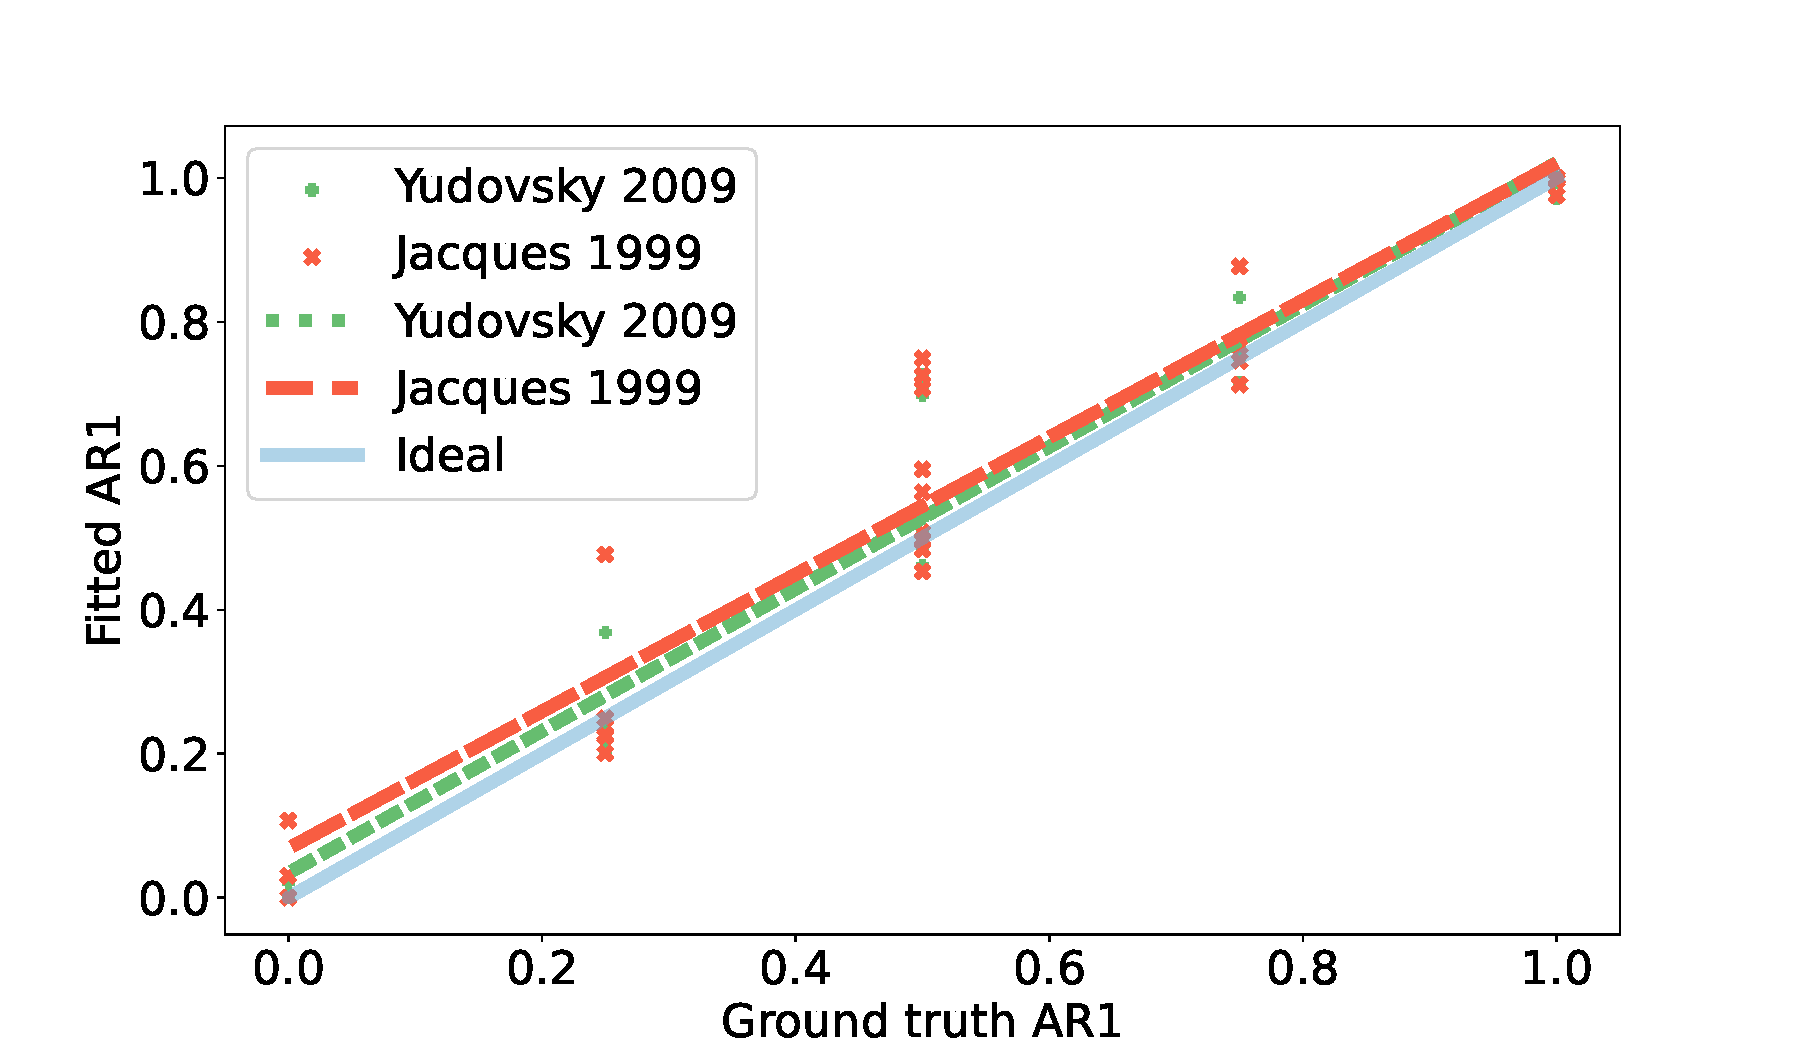
\includegraphics[width=\textwidth]{backwardsPQann.pdf}
        \caption{}
        \label{fig:backwardsPQann}
    \end{subfigure}
    \begin{subfigure}{0.49\textwidth}
        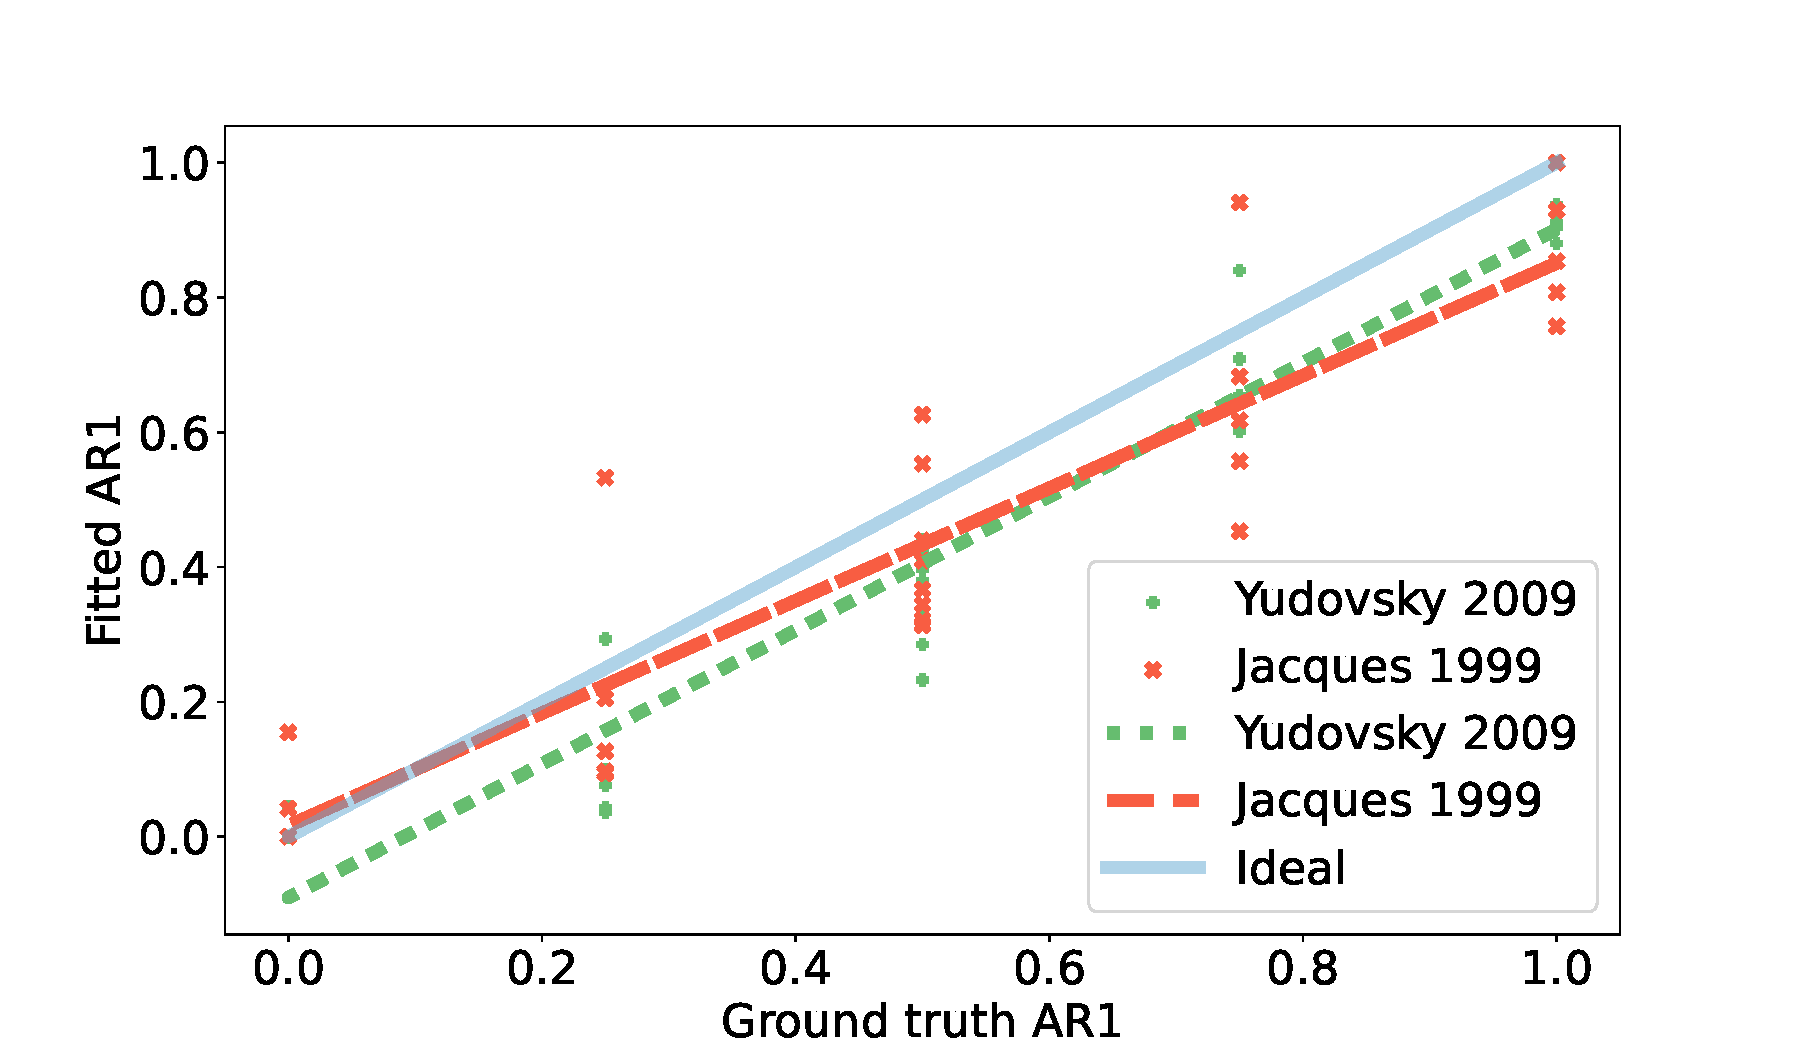
\includegraphics[width=\textwidth]{backwardsPRann.pdf}
        \caption{}
        \label{fig:backwardsPRann}
    \end{subfigure}
    \begin{subfigure}{0.49\textwidth}
        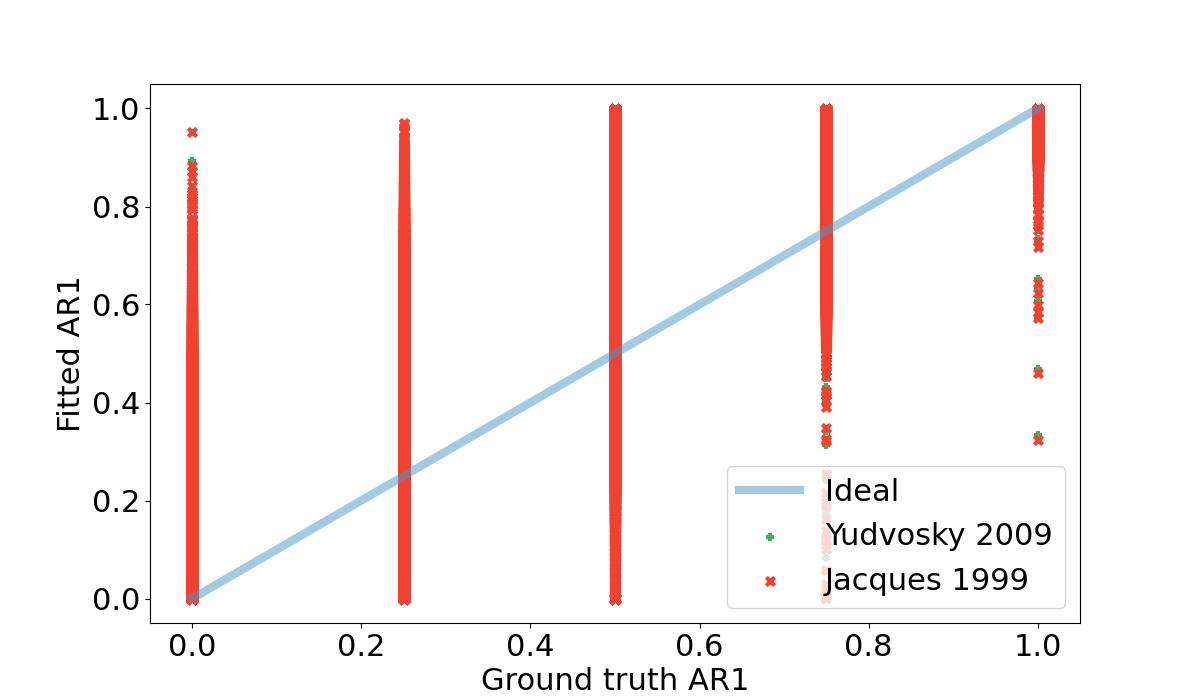
\includegraphics[width=\textwidth]{backwardsPQpbp.pdf}
        \caption{}
        \label{fig:backwardsPQpbp}
    \end{subfigure}
    \begin{subfigure}{0.49\textwidth}
        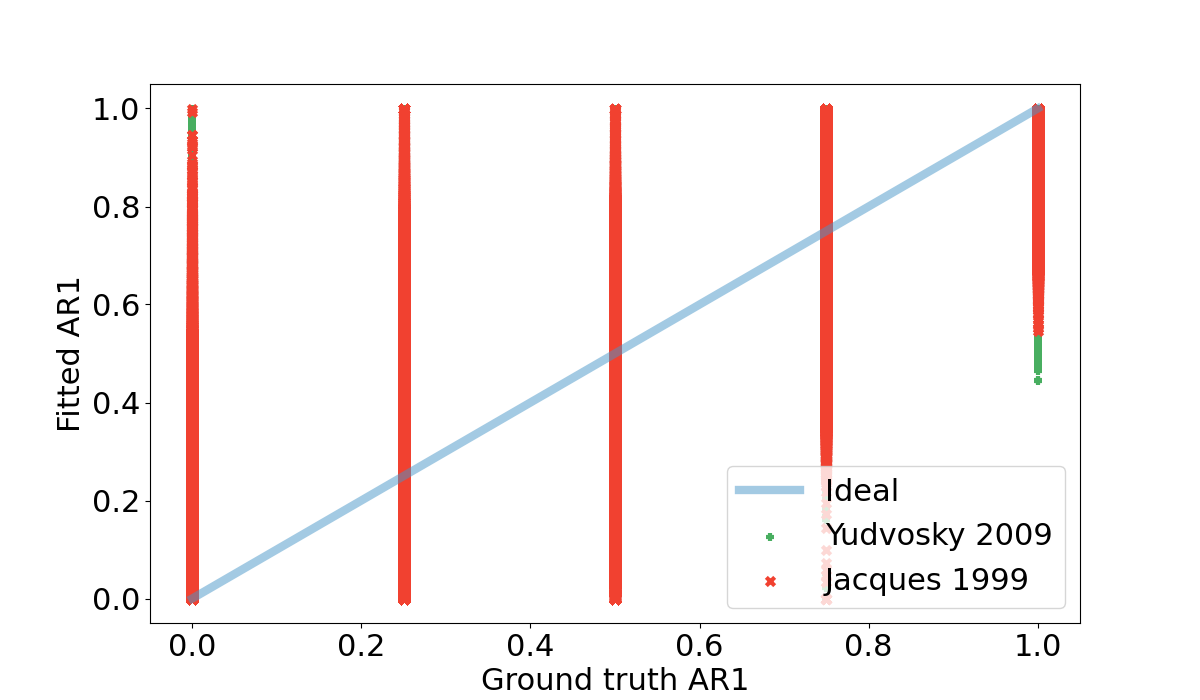
\includegraphics[width=\textwidth]{backwardsPRpbp.pdf}
        \caption{}
        \label{fig:backwardsPRpbp}
    \end{subfigure}
    \begin{subfigure}{0.49\textwidth}
        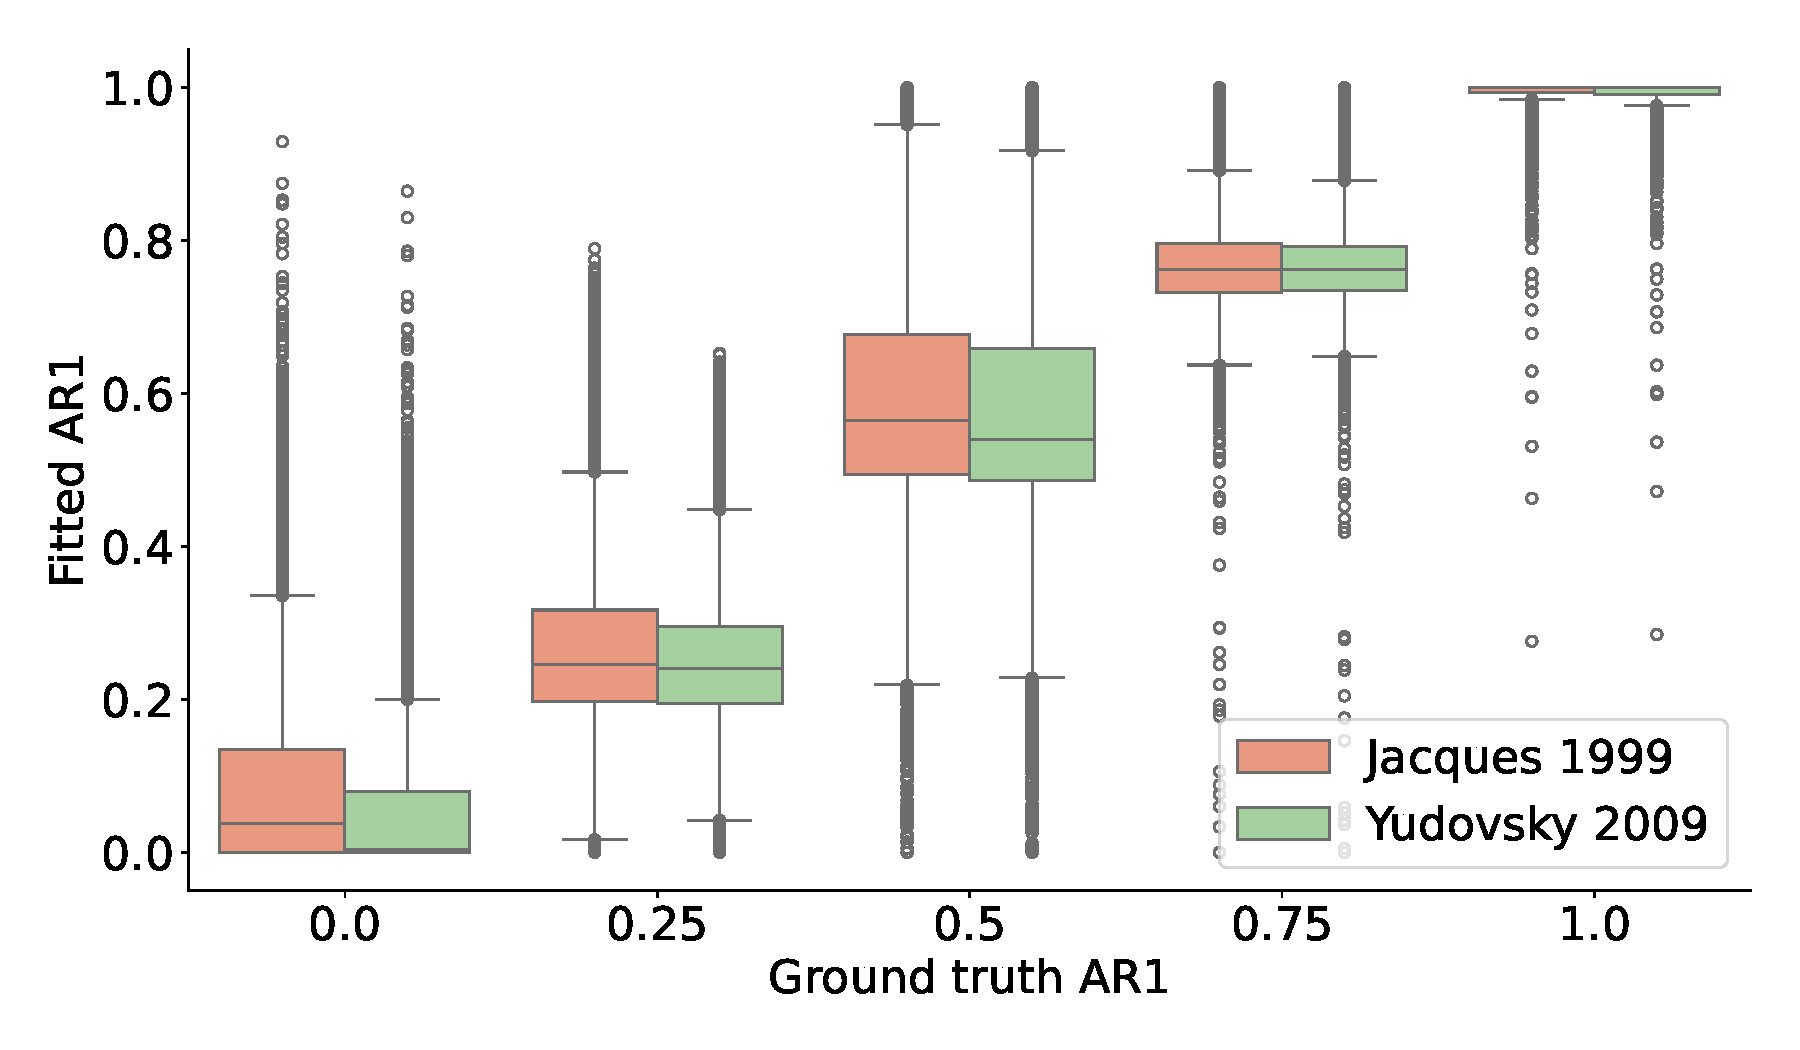
\includegraphics[width=\textwidth]{backwardsPQpbp5.pdf}
        \caption{}
        \label{fig:backwardsPQpbp5}
    \end{subfigure}
    \begin{subfigure}{0.49\textwidth}
        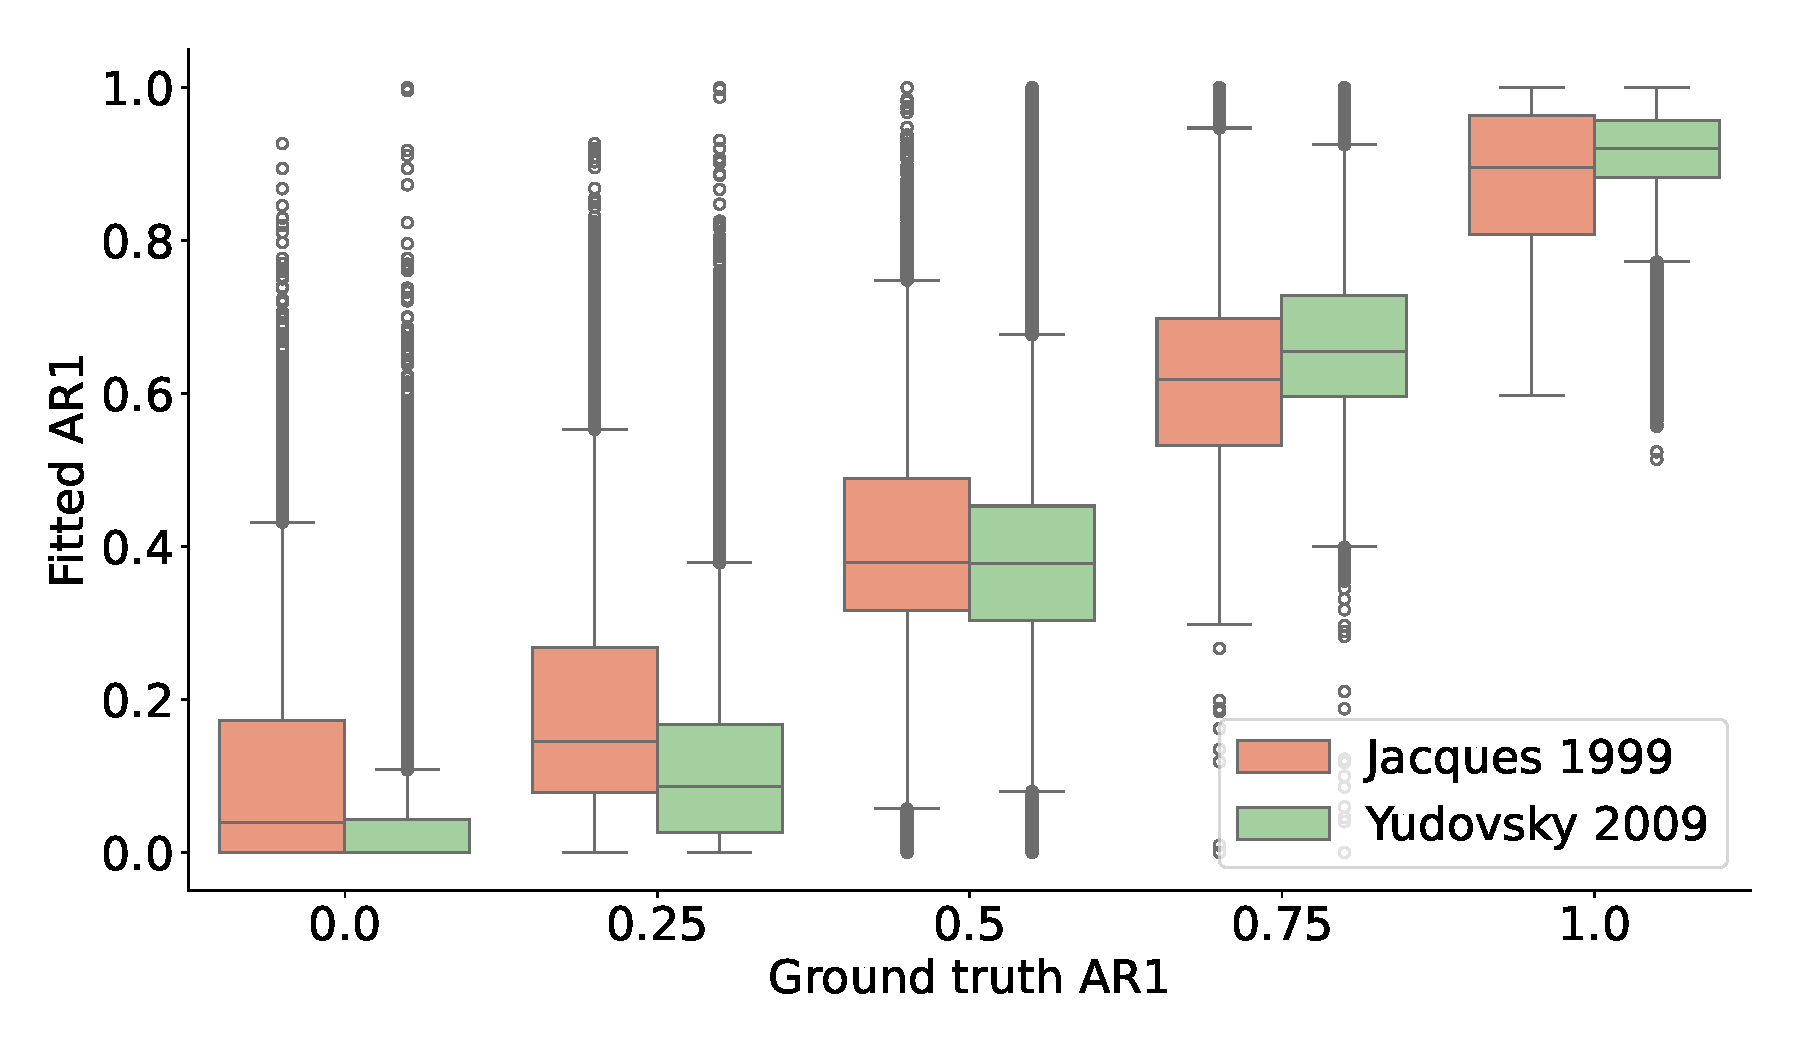
\includegraphics[width=\textwidth]{backwardsPRpbp5.pdf}
        \caption{}
        \label{fig:backwardsPRpbp5}
    \end{subfigure}
    \caption{An example of the quality of parameter recovery by fitting each inverse analytical model (Yudovsky 2009 (\textcolor{MyGreen}{green $+$}) and Jacques 1999 (\textcolor{MyOrange}{orange $\times$})) to the quantitative (left) or relative (right) mean annotated spectra from 1 frame (top) or pixel-by-pixel in the annotated region from 1 frame (middle) or the mean of 5 frames (bottom) from each video of the HSI phantom dataset and their associated trend lines using a refractive index of 1.35 for $AR1$.}
    \label{fig:backwardsHSIphantomsann}
\end{figure}

\begin{figure}[h!]
    \centering 
    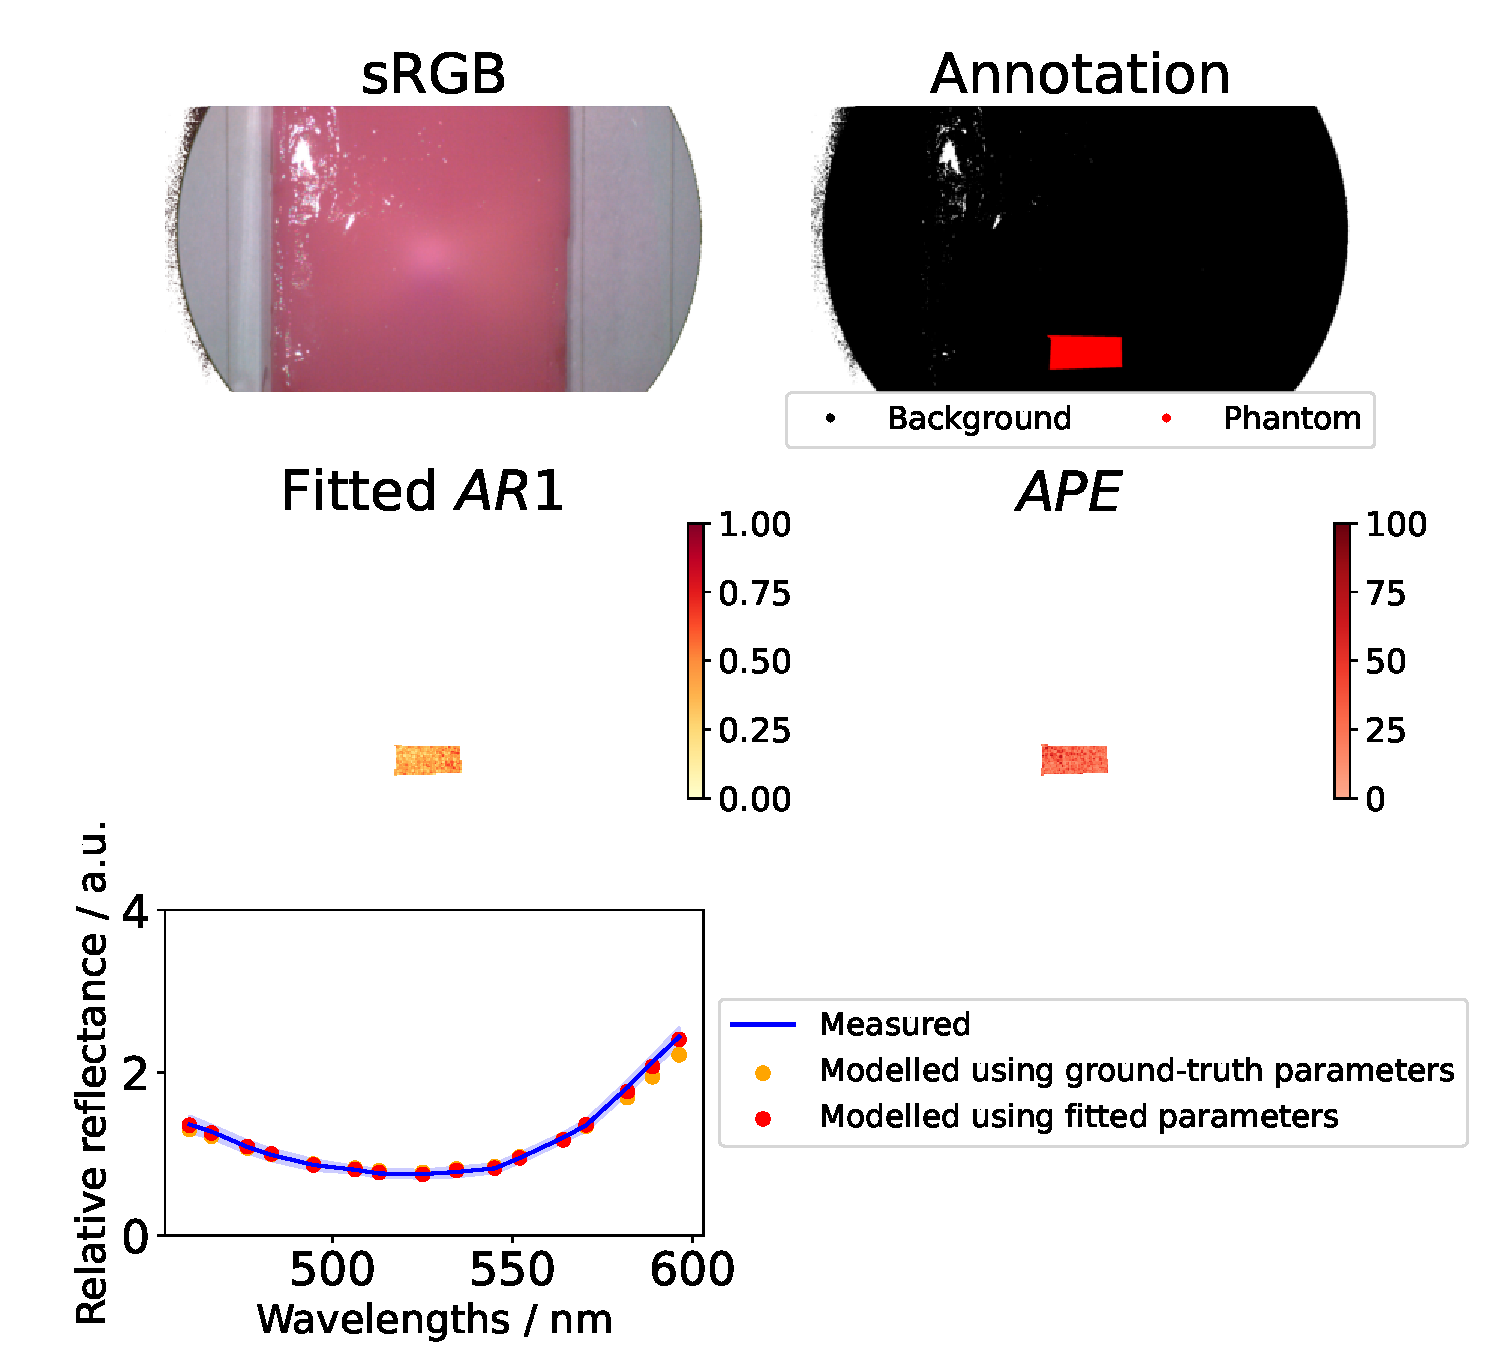
\includegraphics[width=\textwidth]{7_350_Y_ON_AR1.pdf}
    \caption{Top left shows an sRGB reconstruction of a frame of a hyperspectral video of a gelatin-based phantom where $AR1=0.5$ and $I=3.50\%$ taken with a snapshot HSI camera, where the regions beyond thresholds are shown as white. Top right shows an annotation of the same image. Middle left shows the fitted $StO_2$ on a pixel-by-pixel basis of the relative data using the Yudovsky 2009 single-layer model. Middle right shows the $APE$ of the fitted $AR1$ of each pixel in the annotated region compared to the ground truth value (0.5). Bottom shows the mean annotated spectrum ($\pm$ standard deviation) plotted with the modelled spectrum using ground-truth parameters or parameters fitted to the mean annotated spectrum.}
    \label{fig:gelatinpbpeg}
\end{figure}

\begin{figure}[h!]
    \centering 
    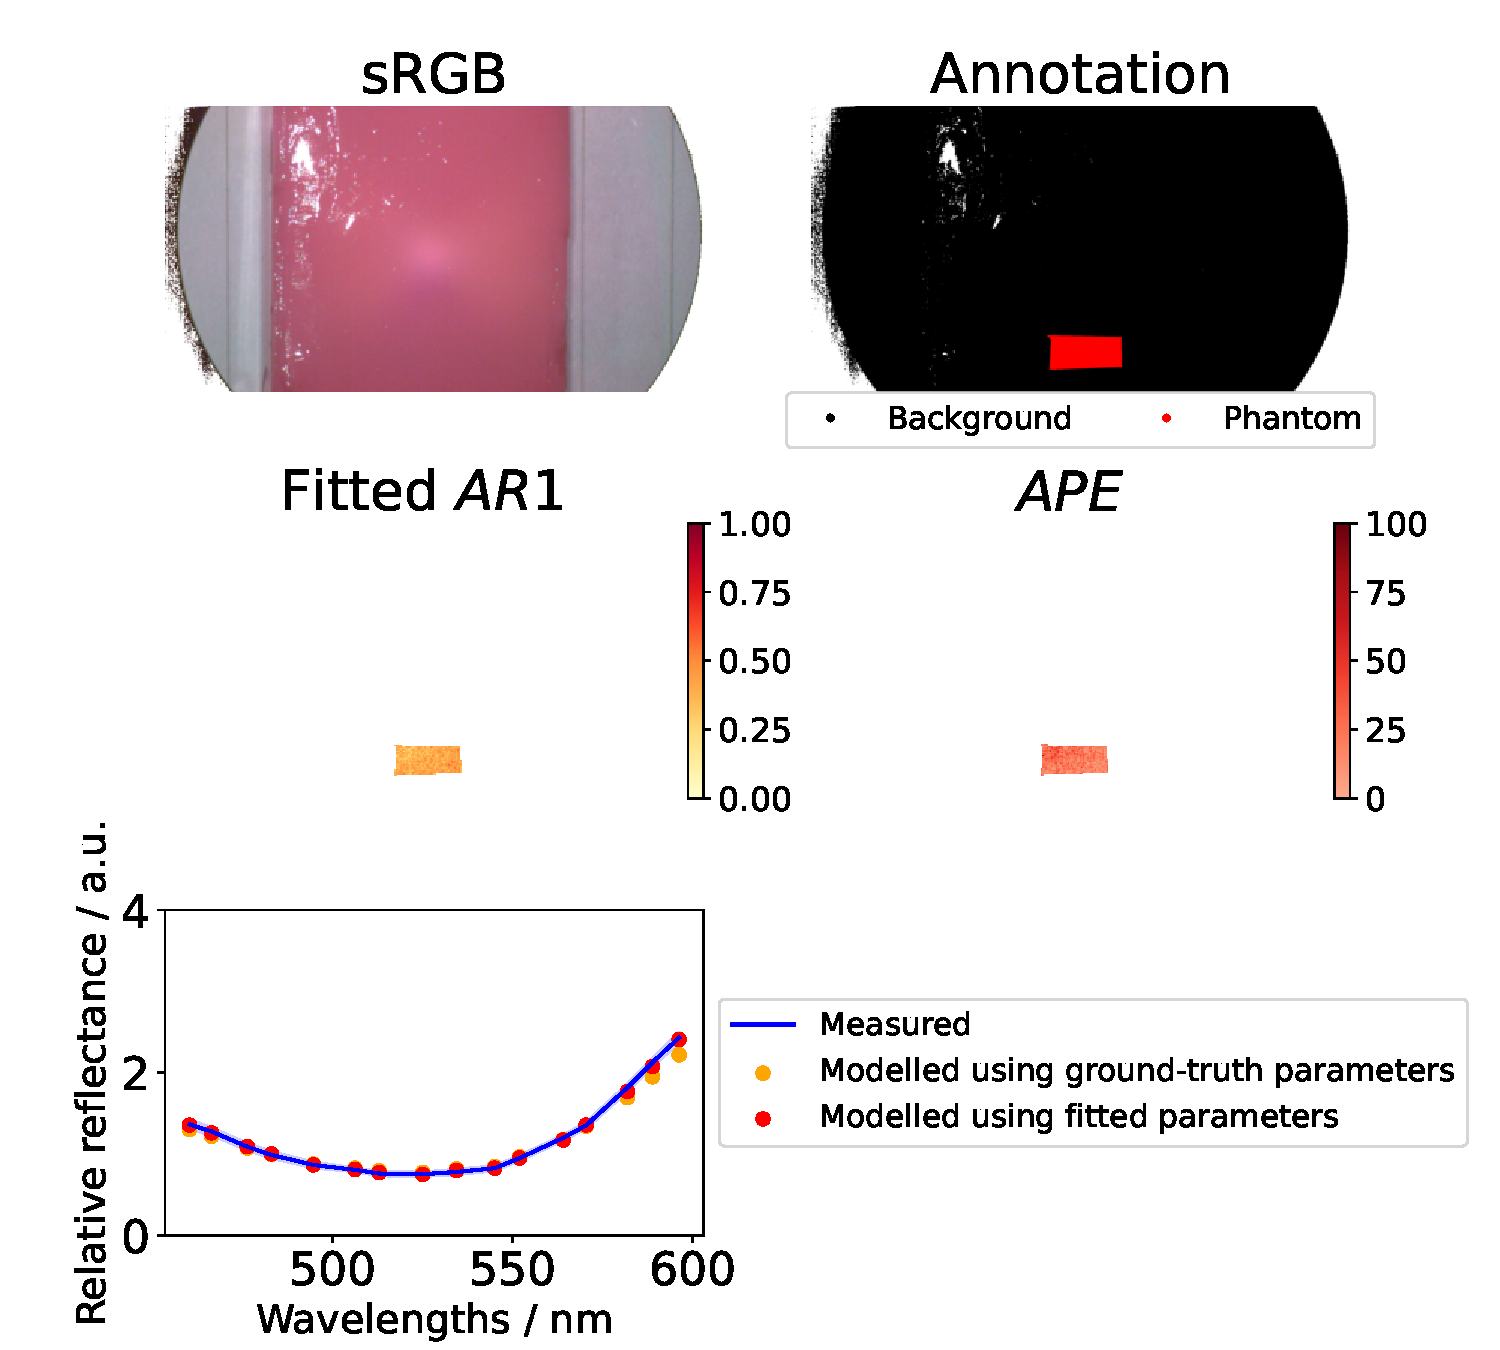
\includegraphics[width=\textwidth]{7_350_Y_ON_AR1_5.pdf}
    \caption{Top left shows an sRGB reconstruction of the mean of 5 frames of a hyperspectral video of a gelatin-based phantom where $AR1=0.5$ and $I=3.50\%$ taken with a snapshot HSI camera, where the regions beyond thresholds are shown as white. Top right shows an annotation of the same image. Middle left shows the fitted $StO_2$ on a pixel-by-pixel basis of the relative data using the Yudovsky 2009 single-layer model. Middle right shows the $APE$ of the fitted $AR1$ of each pixel in the annotated region compared to the ground truth value (0.5). Bottom shows the mean annotated spectrum ($\pm$ standard deviation) plotted with the modelled spectrum using ground-truth parameters or parameters fitted to the mean annotated spectrum.}
    \label{fig:gelatinpbpeg5}
\end{figure}

\FloatBarrier
\subsection{Neurosurgical HSI data}
The Yudovsky 2009 and Jacques 1999 single layer models are fitted to neurosurgical HSI data since Chapters \ref{chap:1layer} and \ref{chap:2layer} and Section \ref{sec:MCHSI} shows these are more robust.
%to reduction in the number of available wavelengths 
%and meningial layers in these images are largely considered sufficiently low scattering, absorbance, and thickness as to be negligible \textcolor{red}{try to reference this}. 
This makes the assumption that the impact of the meninges is sufficiently small as to be negligible. Whilst the arachnoid and pia layers are known to have scattering and absorbance properties, they are very thin layers and so appear highly transparent allowing this assumption to be made~\citep{Ghannam2023}.
The relative mean annotated spectra for each tissue type of each image in the HELICoiD dataset is used for fitting each model using the literature or shifted extinction coefficients and the resulting mean (standard deviation) physiological parameters are shown in Table \ref{tb:HELICoiD}. Examples of fitted spectra using each model and the distribution for $StO_2$ are shown in Figure \ref{fig:HELICoiDann}. These show very large variation in the extracted $StO_2$. Since there are no known ground truth values for these images, these ranges are compared to JVOS and cerebral oximetry values. Typical JVOS values are quoted to be 55-75\%~\citep{Raith2020, Zhong2021} and would be the lowest $StO_2$ values to be expected as this venous blood is measured after having delivered oxygen to the brain. There is no consensus on typical cerebral oximetry values, however it has been suggested that values below 59\% would indicate cerebral ischaemia~\citep{Zhong2021} and studies have shown ranges of around 60-75\% to be within the normal range~\citep{Lian2020}. This measure does not discriminate between tissue types as there is no spatial resolution, therefore it can be influenced by any tissue type. As displayed in Figure \ref{fig:HELICoiDann}, many recovered values are below these ranges suggesting that the optical modelling of these tissues should be improved. Similar results when analysing the same data using a uniform wavelength weighting function can be found in Appendix \ref{ap:Chapter5uniform}.

\begin{table}[h!]
    \centering
    \caption{The mean (standard deviation) of the fitted physiological parameters when extracted by fitting Yudovsky 2009 single layer (Y) or Jacques 1999 (J) to the relative mean annotated spectra for each tissue type of each image from the HELICoiD dataset using literature (L) or shifted (S) extinction coefficients and $n=1.44$. All presented to 3s.f.}
    \begin{tabular}{|ccc|cccc|}
        \hline
        \multirow{2}{*}{Tissue type} & \multirow{2}{*}{Model} & \multirow{2}{*}{Method} & $StO_2$ & $f_{blood}$ & $a$ & $b$ \\
        & & & (\%) & (\%) & ($cm^{-1}$) & (a.u.) \\
        \hline
        \multirow{4}{*}{\shortstack{Hyper-\\vascularised}} & \multirow{2}{*}{Y} & L & 55.0 (12.6) & 1.94 (1.42) & 47.5 (29.9) & 1.23 (1.15) \\
        & & S & 62.3 (17.5) & 3.21 (3.09) & 67.3 (11.7) & 1.69 (1.22) \\
        \cline{2-7}
        & \multirow{2}{*}{J} & L & 60.1 (19.8) & 23.1 (35.9) & 44.3 (30.8) & 1.40 (1.16) \\
        & & S & 61.1 (17.0) & 5.13 (9.52) & 41.6 (30.2) & 1.84 (1.17) \\
        \hline
        \multirow{4}{*}{Normal} & \multirow{2}{*}{Y} & L & 56.0 (17.1) & 0.719 (0.390) & 10.3 (11.2) & 0.302 (0.783) \\
        & & S & 64.9 (17.2) & 0.684 (0.349) & 8.91 (3.52) & 0.338 (0.801) \\
        \cline{2-7}
        & \multirow{2}{*}{J} & L & 59.1 (20.2) & 0.917 (1.13) & 10.6 (11.3) & 0.301 (0.780) \\
        & & S & 68.1 (19.4) & 0.777 (0.623) & 8.65 (2.70) & 0.327 (0.799) \\
        \hline
        \multirow{4}{*}{Tumour} & \multirow{2}{*}{Y} & L & 60.5 (18.0) & 1.21 (1.38) & 13.7 (18.7) & 0.100 (0.00) \\
        & & S & 69.5 (15.1) & 1.03 (0.902) & 15.4 (18.5) & 0.327 (0.303) \\
        \cline{2-7}
        & \multirow{2}{*}{J} & L & 62.8 (19.6) & 1.17 (0.975) & 8.23 (0.675) & 0.127 (0.0883) \\
        & & S & 70.9 (16.2) & 1.03 (0.754) & 11.6 (4.93) & 0.285 (0.427) \\
        \hline
    \end{tabular}    
    \label{tb:HELICoiD}
\end{table}

\begin{figure}[h!]
    \centering
    \begin{subfigure}{0.49\textwidth}
        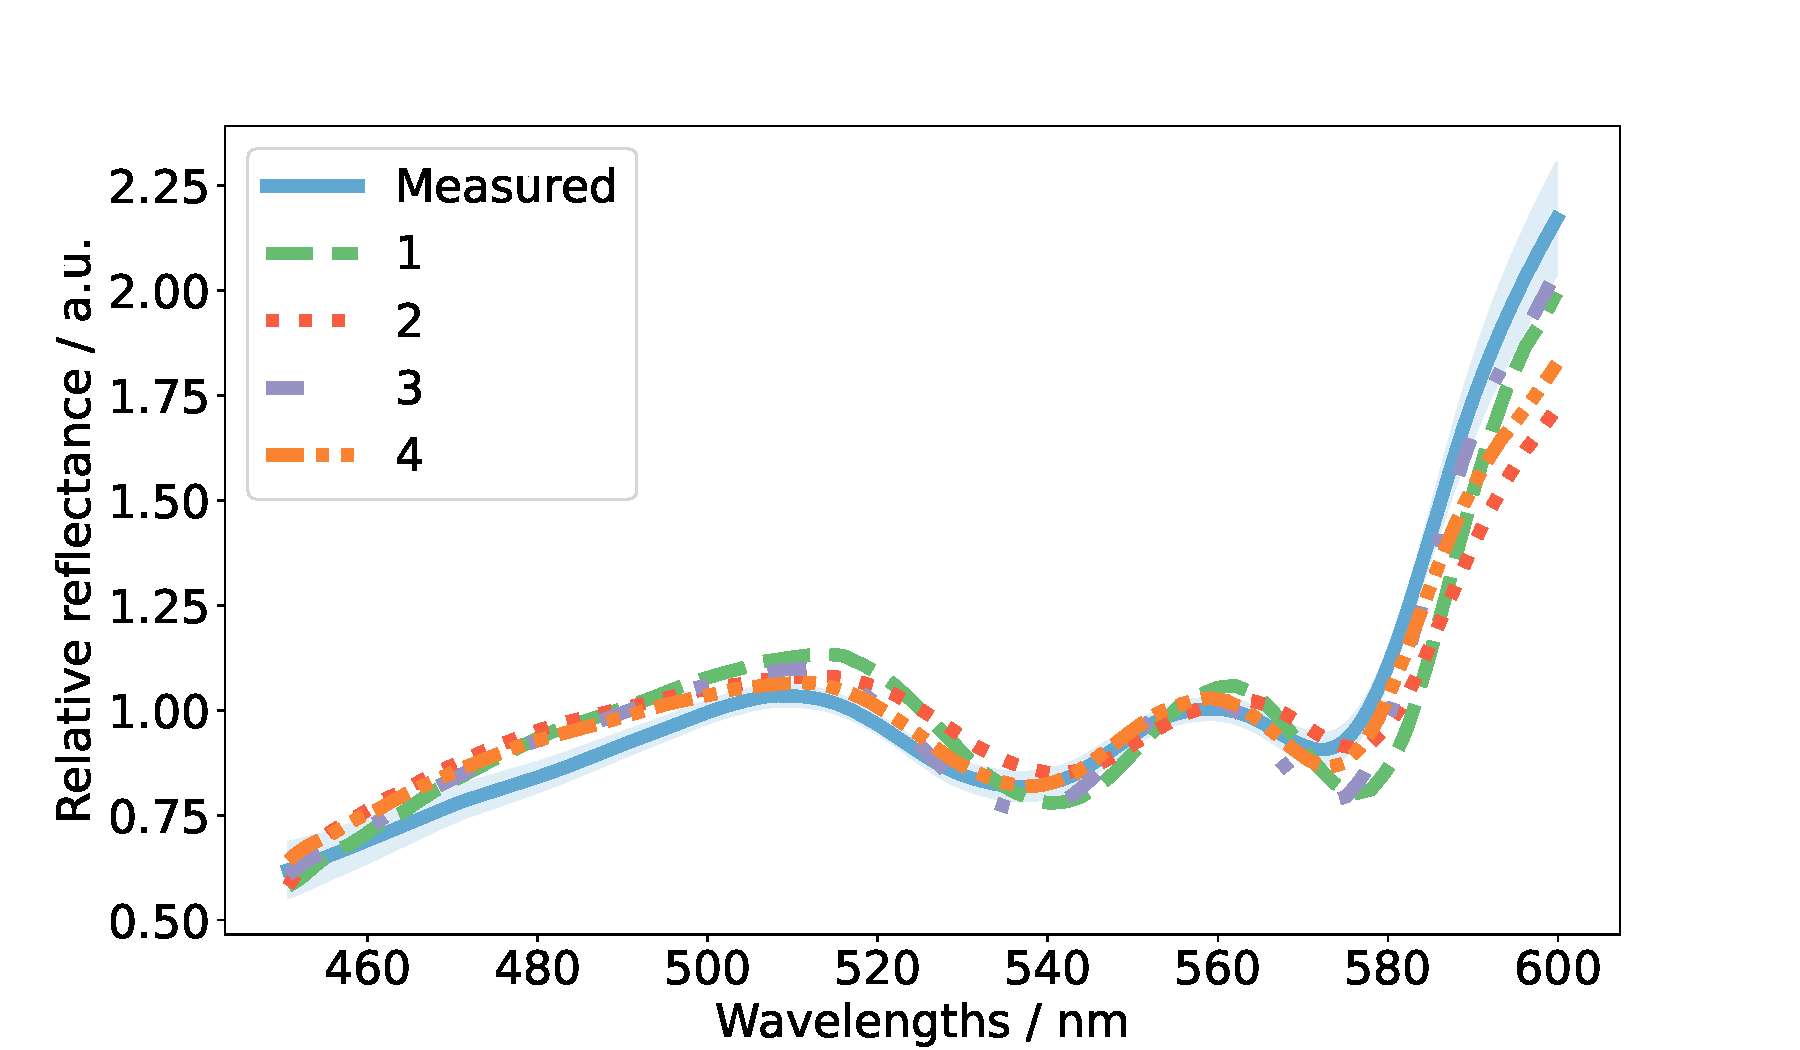
\includegraphics[width=\textwidth]{012-02Normal_spectra_Y.pdf}
        \caption{}
        \label{fig:backwardsHSIHeliY}
    \end{subfigure}
    \begin{subfigure}{0.49\textwidth}
        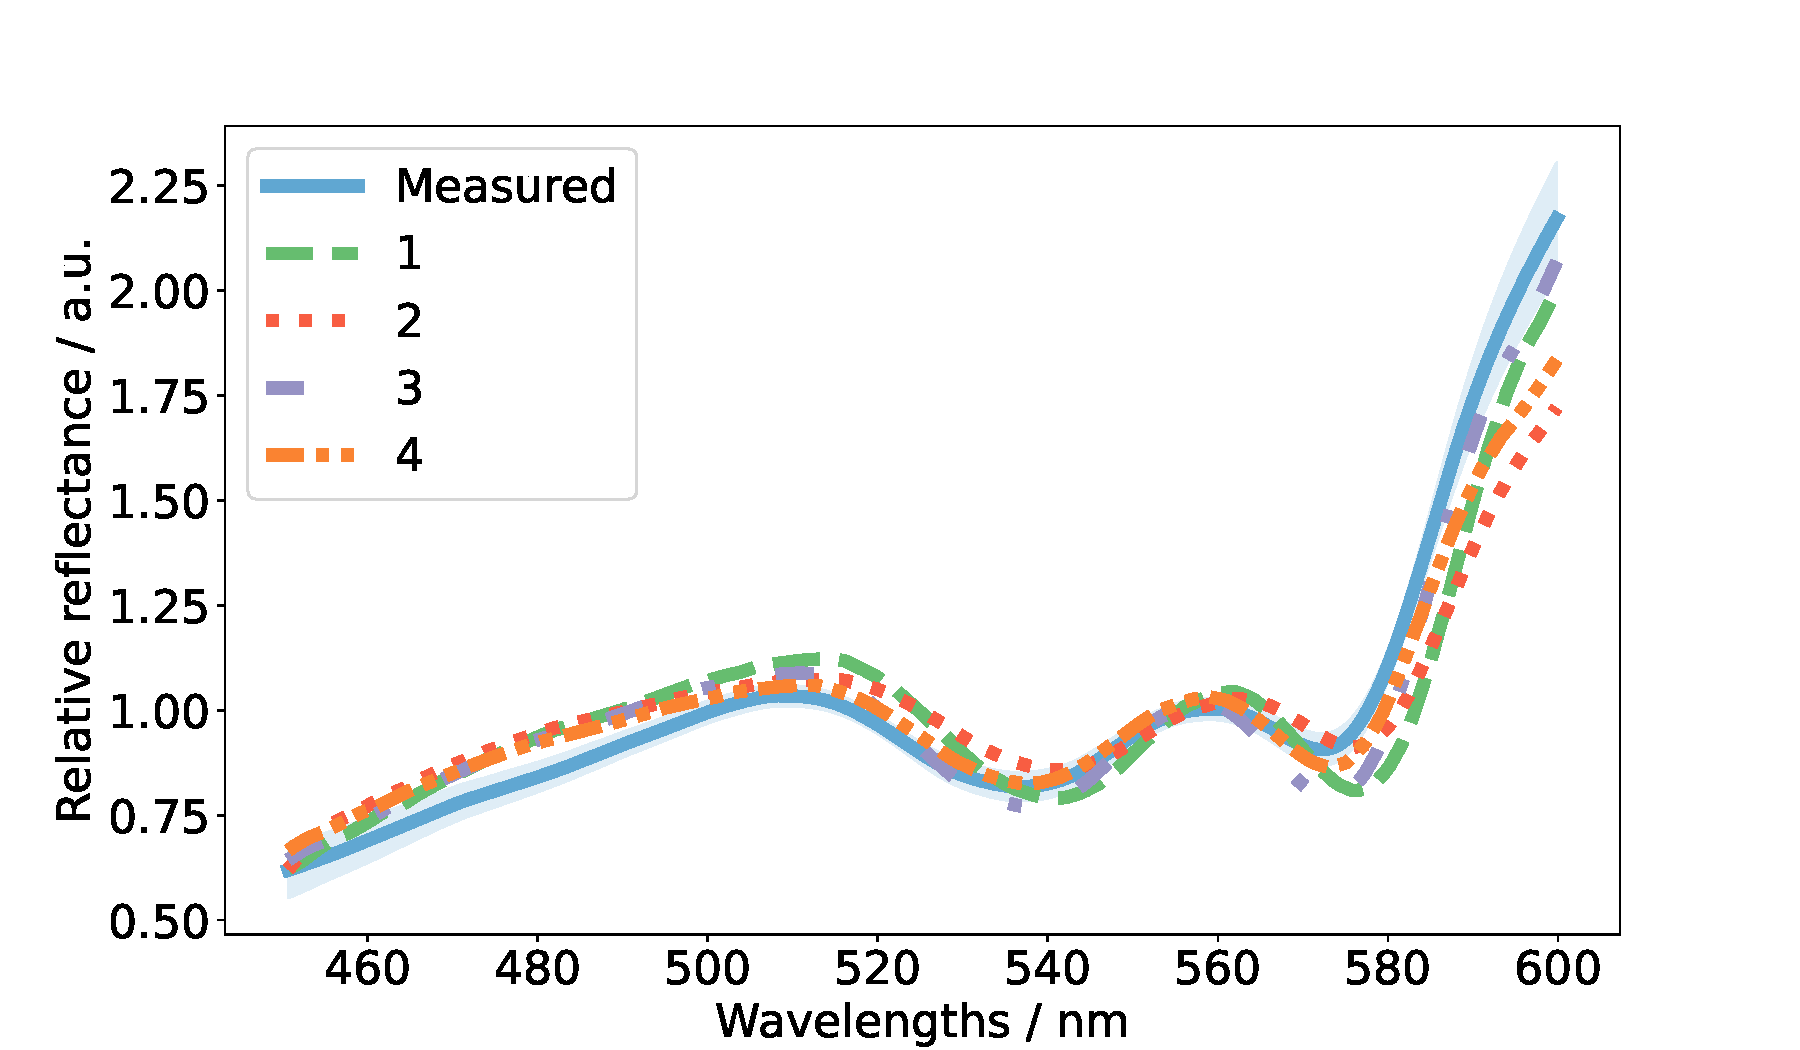
\includegraphics[width=\textwidth]{012-02Normal_spectra_J.pdf}
        \caption{}
        \label{fig:backwardsHSIHeliJ}
    \end{subfigure}
    \begin{subfigure}{\textwidth}
        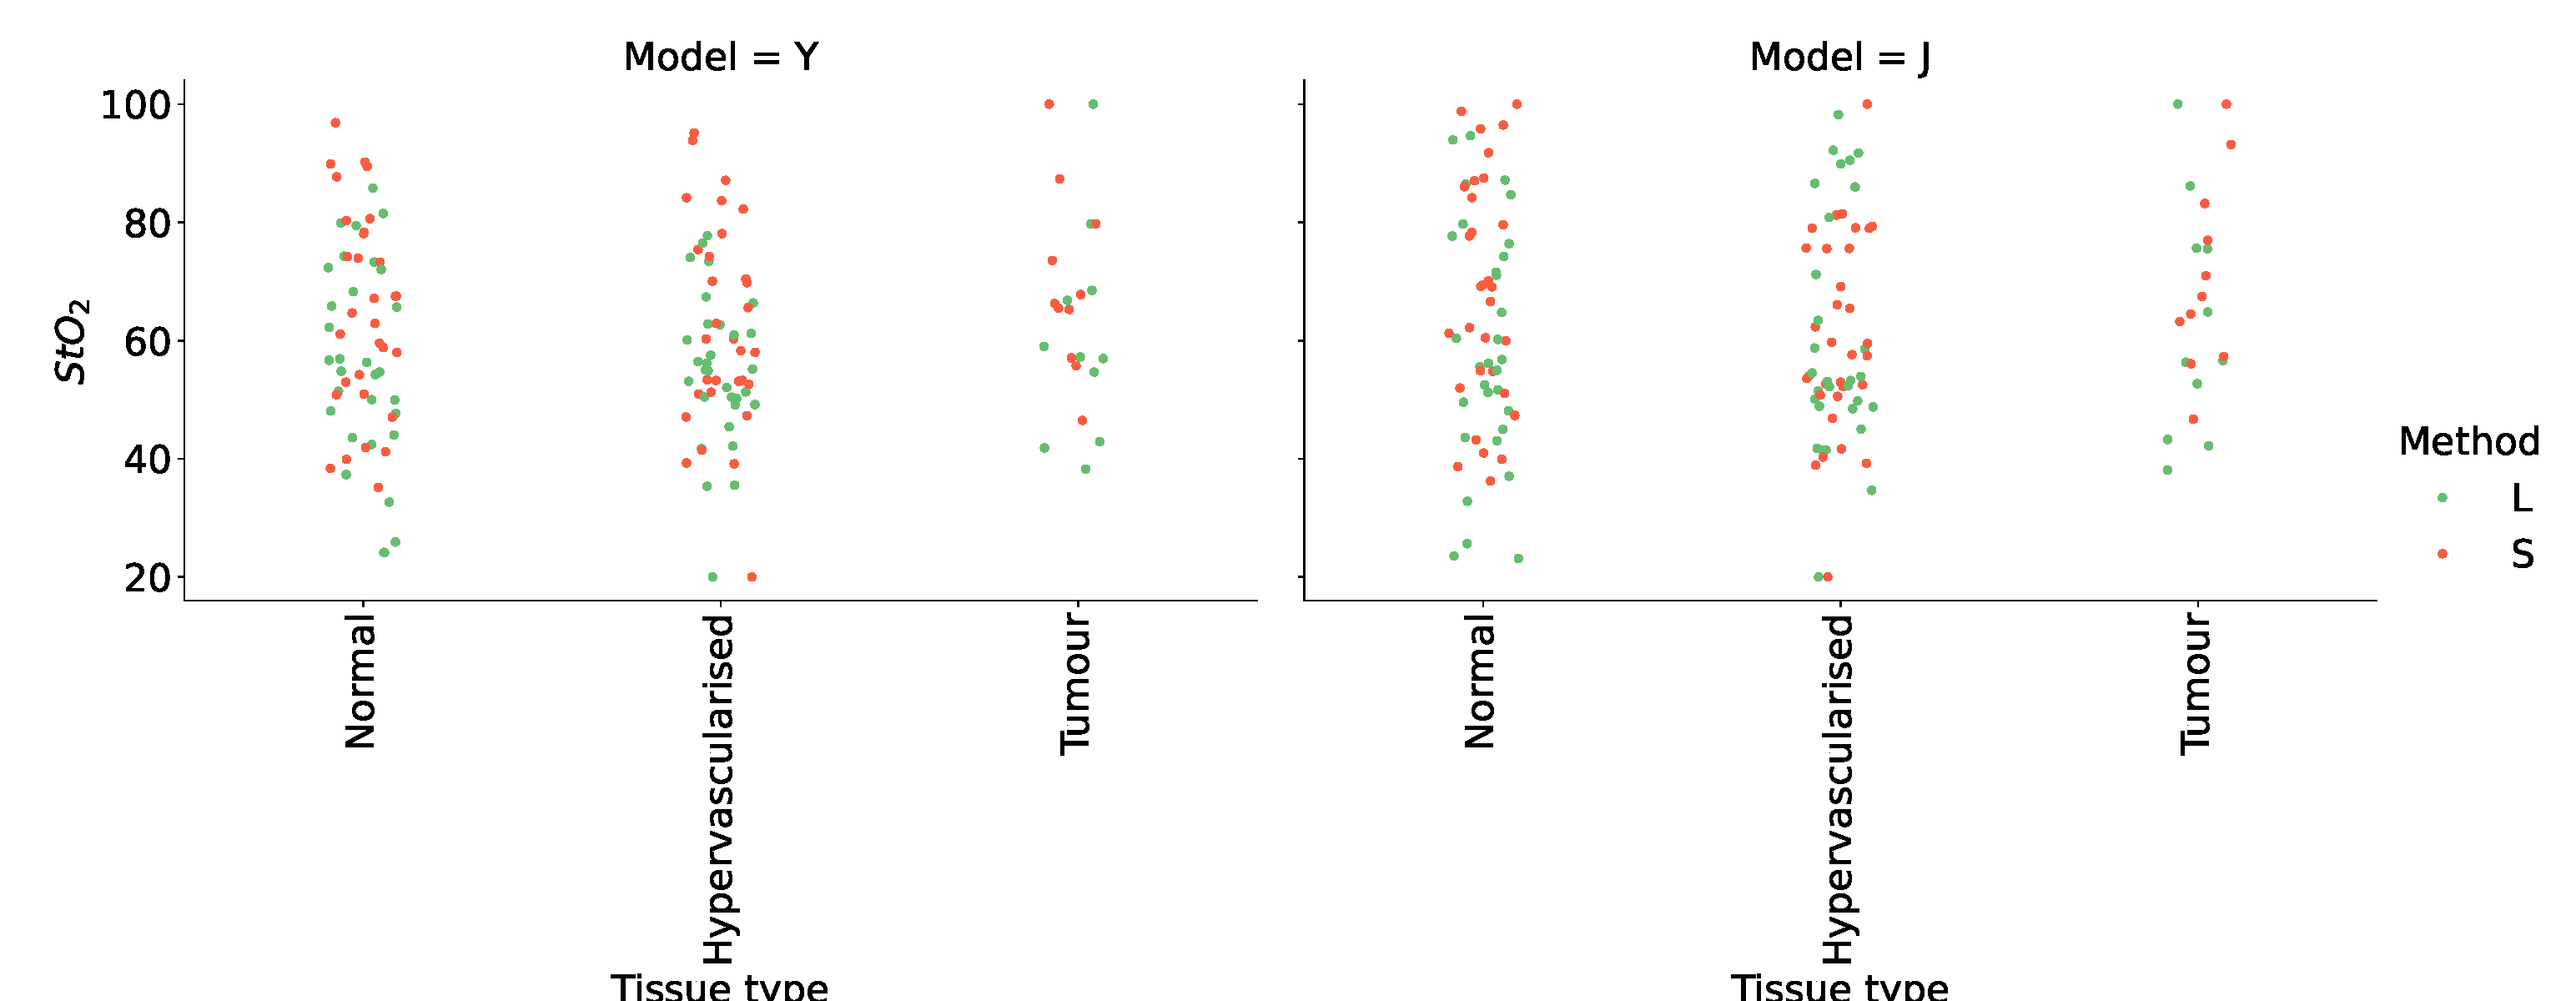
\includegraphics[width=\textwidth]{boxplotsHeli.pdf}
        \caption{}
        \label{fig:boxplotsHeli}
    \end{subfigure}
    \caption{An example of the visual fitting quality of the Yudovsky 2009 (\ref{fig:backwardsHSIHeliY}) and Jacques 1999 (\ref{fig:backwardsHSIHeliJ}) single layer models when fitting to the relative mean annotated spectrum ($\pm$1 standard deviation, \textcolor{blue}{blue solid}) of the normal tissue class of HELICoiD image 12-02 using literature (L) or shifted (S) extinction coefficients. The distribution of the fitted physiological parameters retrieved by fitting each model to each relative mean annotated spectrum of the tissue classes of each HELICoiD image is shown in \ref{fig:boxplotsHeli}.}
    \label{fig:HELICoiDann}
\end{figure}

%Similarly, the annotations from the NeuroHSI dataset are used to produce relative mean spectra for each tissue type which are also analysed. The resulting physiological parameters are shown in Table \ref{tb:NHSIann} and aggregated across tissue types due to the low number of images of each tissue type. The distribution of $StO_2$ is shown in Figure \ref{tb:NHSIann} which also shows an example of the visual fitting of each model using each method to the mean annotated spectrum of the cortex class of image P010010-T02. Here it is clear that the extracted $StO_2$ values have a very narrow distribution which do not distinguish well between tissue types or images so providing little value. 
%%Likely will need to update the table and figures here when further data is uploaded and/or annotations. 
%
% \begin{table}[h!]
%     \centering
%     \caption{The mean (standard deviation) of the fitted physiological parameters when extracted by fitting Yudovsky 2009 single layer (Y) or Jacques 1999 (J) to the relative mean annotated spectra for each mean annotated spectrum in each image from the NeuroHSI dataset using each method in \ref{sec:NeuroHSIdata} aggregated across all tissue types. All presented to 3s.f.}
%     \begin{tabular}{|cc|cccc|}
%         \hline
%         \multirow{2}{*}{Model} & \multirow{2}{*}{Method} & $StO_2$ & $f_{blood}$ & $a$ & $b$ \\
%         & & (\%) & (\%) & ($cm^{-1}$) & (a.u.) \\
%         \hline
%         \multirow{4}{*}{Y} & 1 & 99.0 (2.45) & 9.40 (8.46) & 39.4 (25.3) & 1.09 (0.368) \\
%         & 2 & 98.6 (8.23) & 8.26 (7.91) & 35.9 (27.5) & 1.31 (0.422) \\
%         & 3 & 100 (4.51$\times 10^{-10}$) & 6.34 (5.34) & 37.9 (24.7) & 1.43 (0.435) \\
%         & 4 & 99.0 (5.20) & 6.15 (4.41) & 53.1 (26.3) & 1.99 (0.546) \\
%         \hline
%         \multirow{4}{*}{J} & 1 & 99.6 (1.58) & 15.2 (9.98) & 65.4 (15.7) & 1.15 (0.476) \\
%         & 2 & 99.1 (5.83) & 14.8 (9.89) & 61.6 (17.6) & 1.53 (0.493) \\
%         & 3 & 99.9 (0.931) & 10.7 (11.1) & 64.0 (17.3) & 1.53 (0.514) \\
%         & 4 & 99.0 (6.06) & 9.33 (13.3) & 54.4 (23.7) & 2.28 (0.617) \\
%         \hline
%     \end{tabular}    
%     \label{tb:NHSIann}
% \end{table}
%
% \begin{figure}[h!]
%     \centering
%     \begin{subfigure}{0.49\textwidth}
%         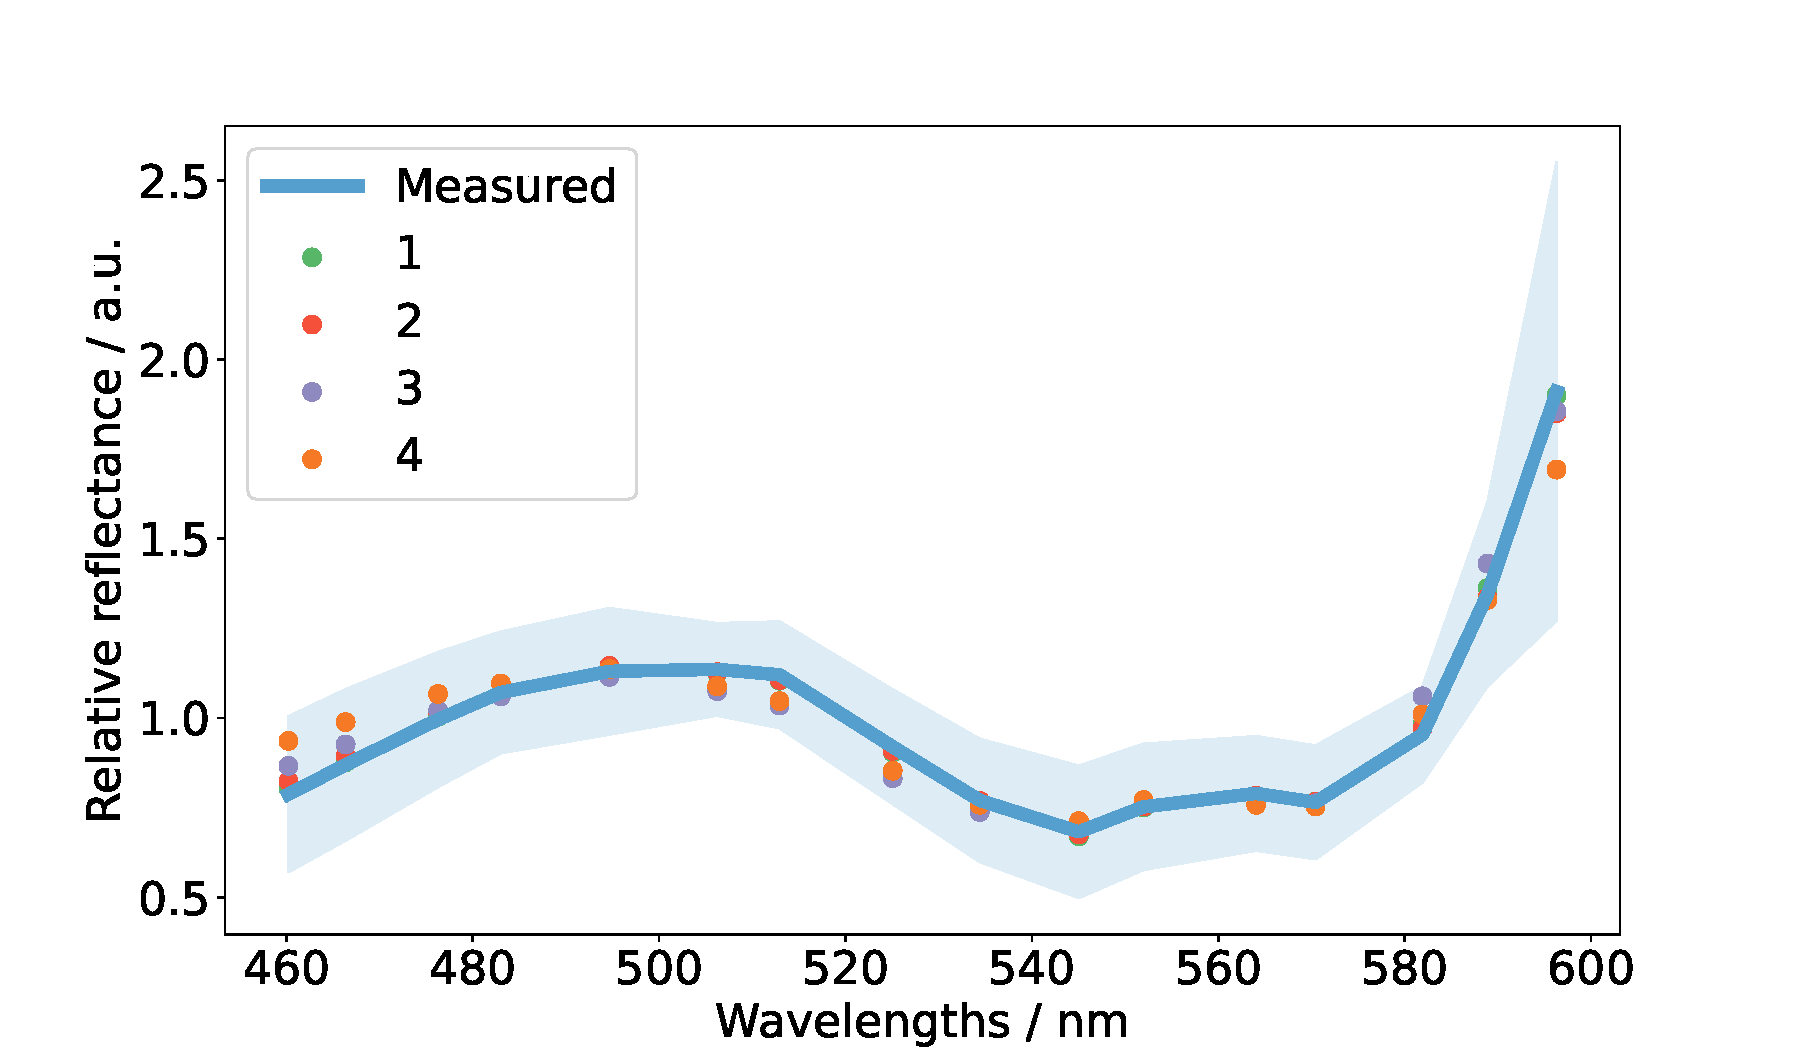
\includegraphics[width=\textwidth]{P010010_T02Cortex_spectra_Y.pdf}
%         \caption{}
%         \label{fig:backwardsHSINHSIY}
%     \end{subfigure}
%     \begin{subfigure}{0.49\textwidth}
%         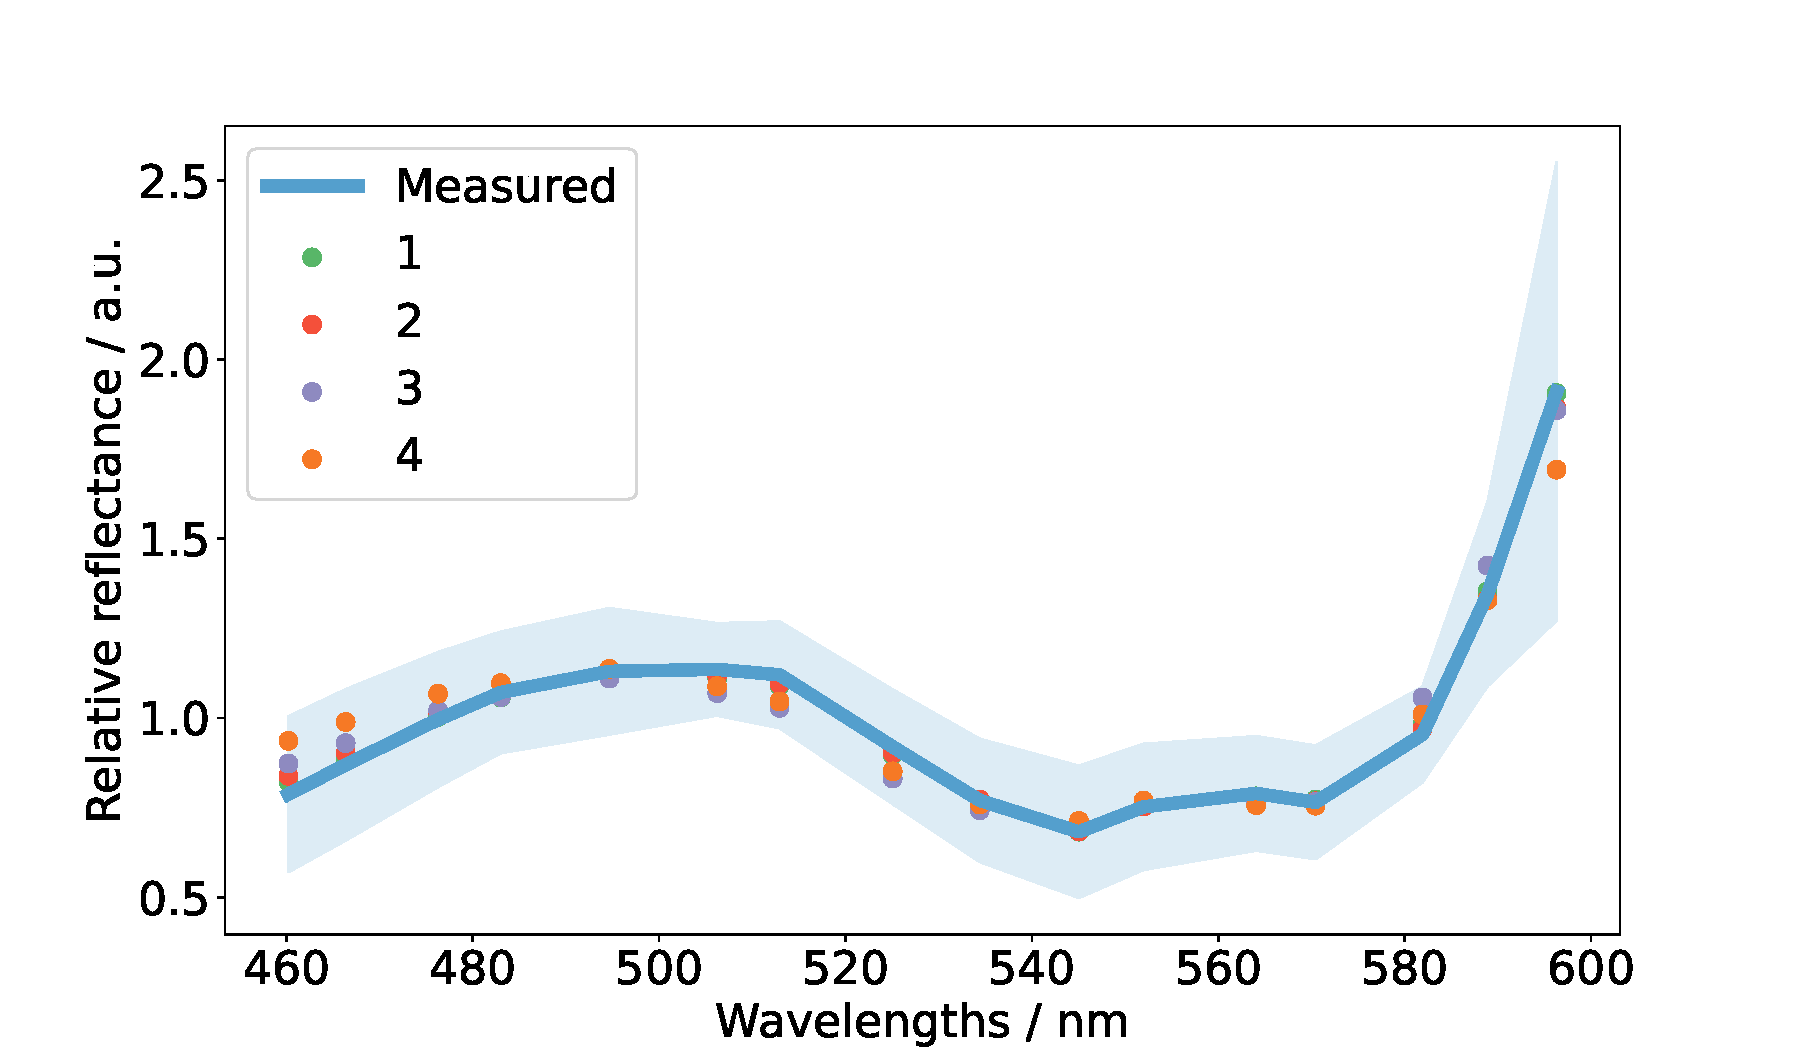
\includegraphics[width=\textwidth]{P010010_T02Cortex_spectra_J.pdf}
%         \caption{}
%         \label{fig:backwardsHSINHSIJ}
%     \end{subfigure}
%     \begin{subfigure}{\textwidth}
%         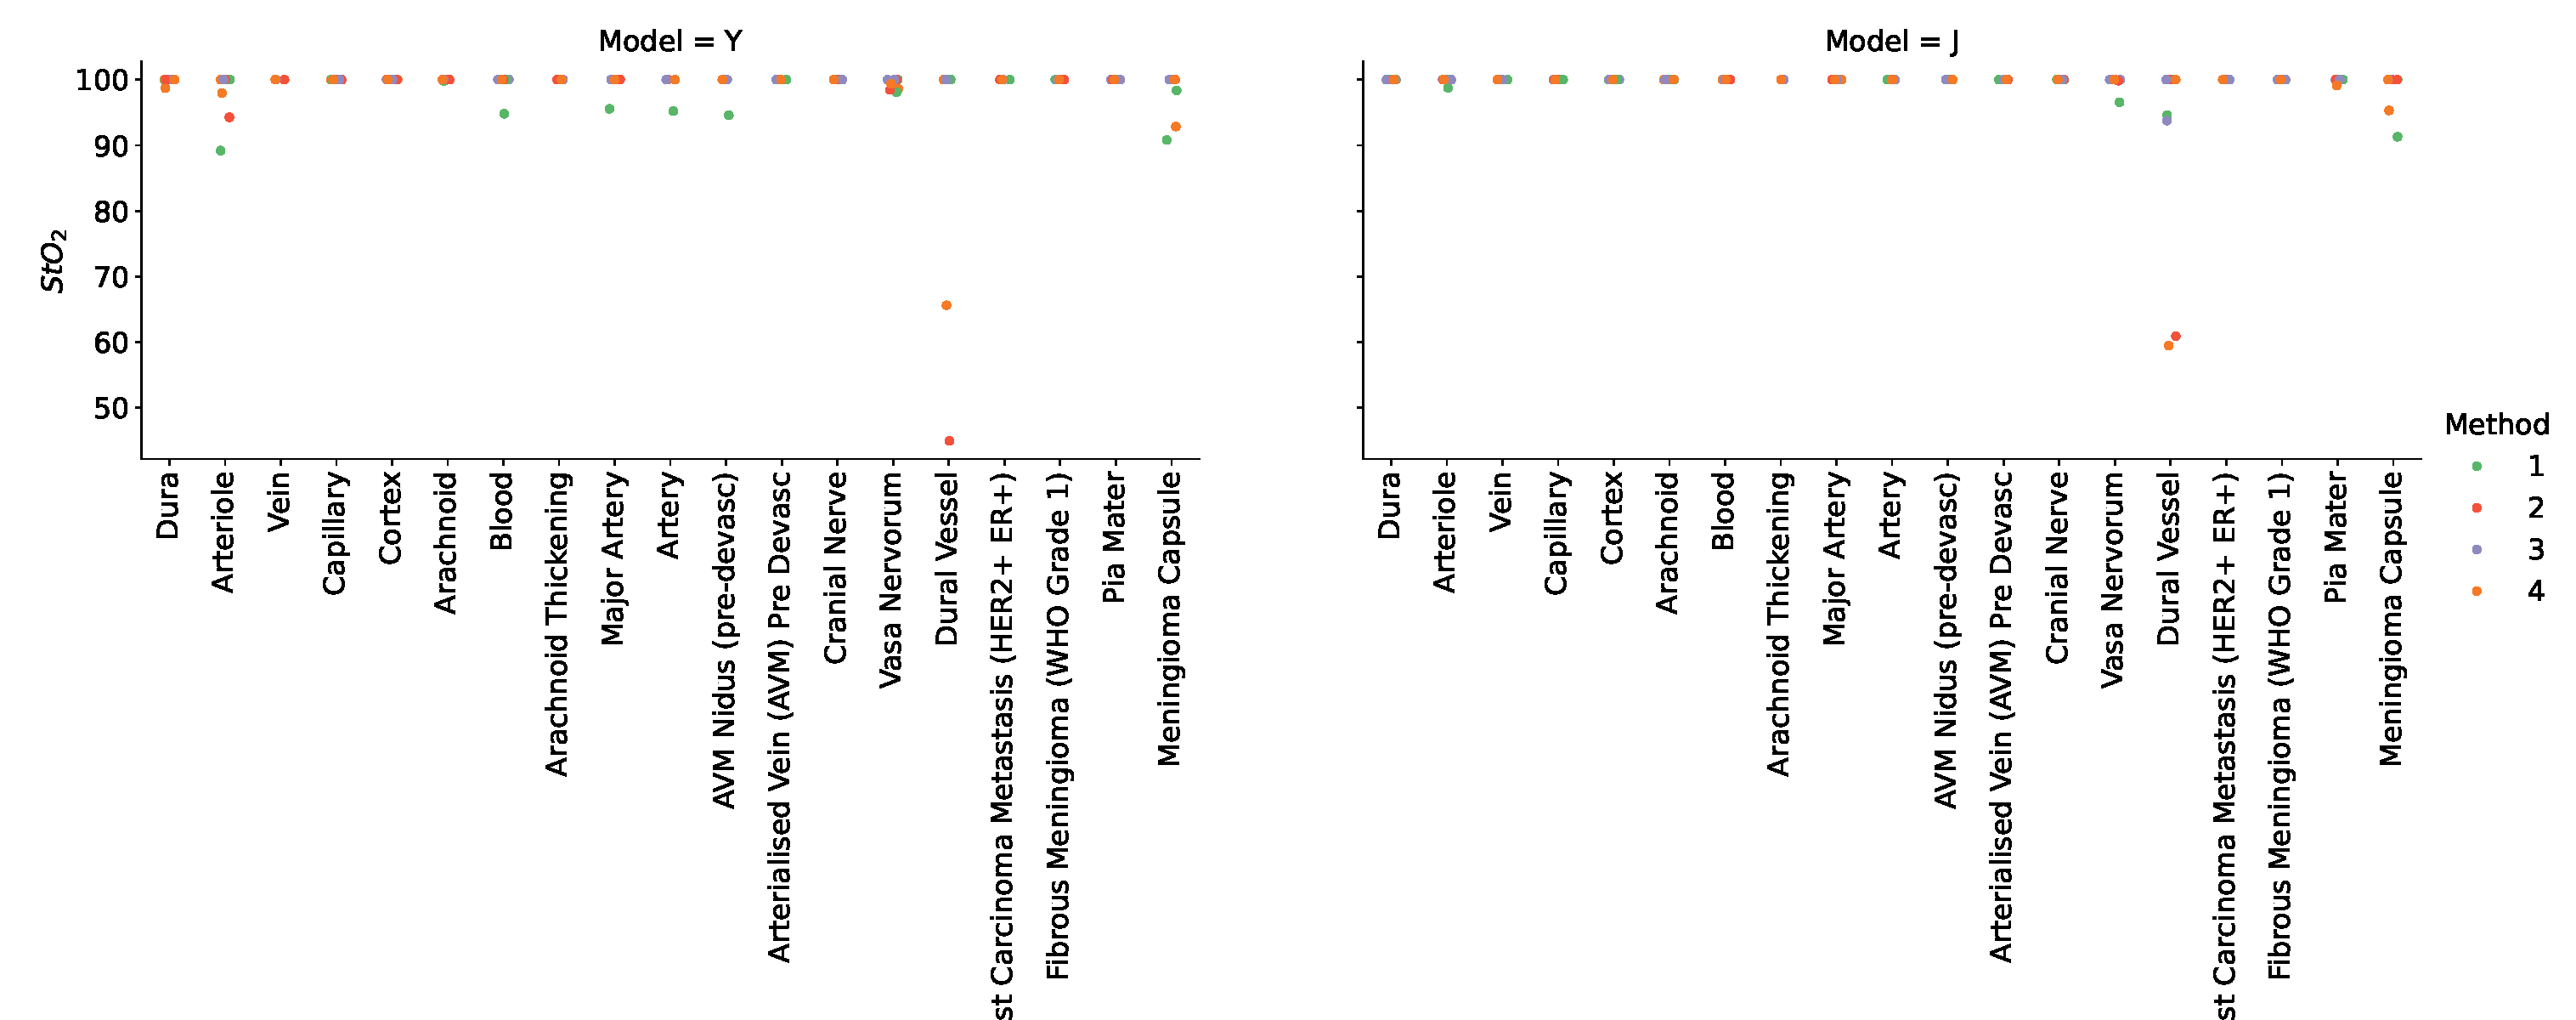
\includegraphics[width=\textwidth]{boxplotsNHSI.pdf}
%         \caption{}
%         \label{fig:boxplotsNHSI}
%     \end{subfigure}
%     \caption{An example of the visual fitting quality of each method in \ref{sec:NeuroHSIdata} used for the Yudovsky 2009 (\ref{fig:backwardsHSINHSIY}) and Jacques 1999 (\ref{fig:backwardsHSINHSIJ}) single layer models when fitting to the relative mean annotated spectrum ($\pm$1 standard deviation, \textcolor{blue}{blue solid}) of the cortex tissue class of NeuroHSI image P010010-T02. The distribution of the fitted physiological parameters retrieved by fitting each model using each method to each relative mean annotated spectrum of the tissue classes of each NeuroHSI image is shown in \ref{fig:boxplotsNHSI}.}
%     \label{fig:NHSIann}
% \end{figure}

The Yudovsky 2009 model is fitted using the Yudovsky 2009 single-layer model with shifted extinction coefficients to HELICoiD image 12-02 on a pixel-by-pixel basis. Figure \ref{fig:HELICoiDpixelY} depicts the resulting $StO_2$ image alongside the sRGB reconstruction of the image and the $APE$ of the $StO_2$ from that obtained by fitting to the mean annotated spectrum within the annotated regions, however this error metric is only calculated in the annotated regions. In all of these plots regions beyond the 99.5\% and 0.5\% thresholds are indicated as white with this extending to all regions outside of the annotated regions in the $APE$ plot. The mean annotated spectrum ($\pm$ standard deviation) for each tissue type in this image is also presented alongside the modelled spectrum using parameters fitted to the mean annotated spectrum in Figure \ref{fig:HELICoiDpixelY}. A similar figure for the Jacques 1999 single-layer model can be seen in Appendix \ref{ap:HELICoiDpixelJ}.

\begin{figure}[h!]
    \centering 
    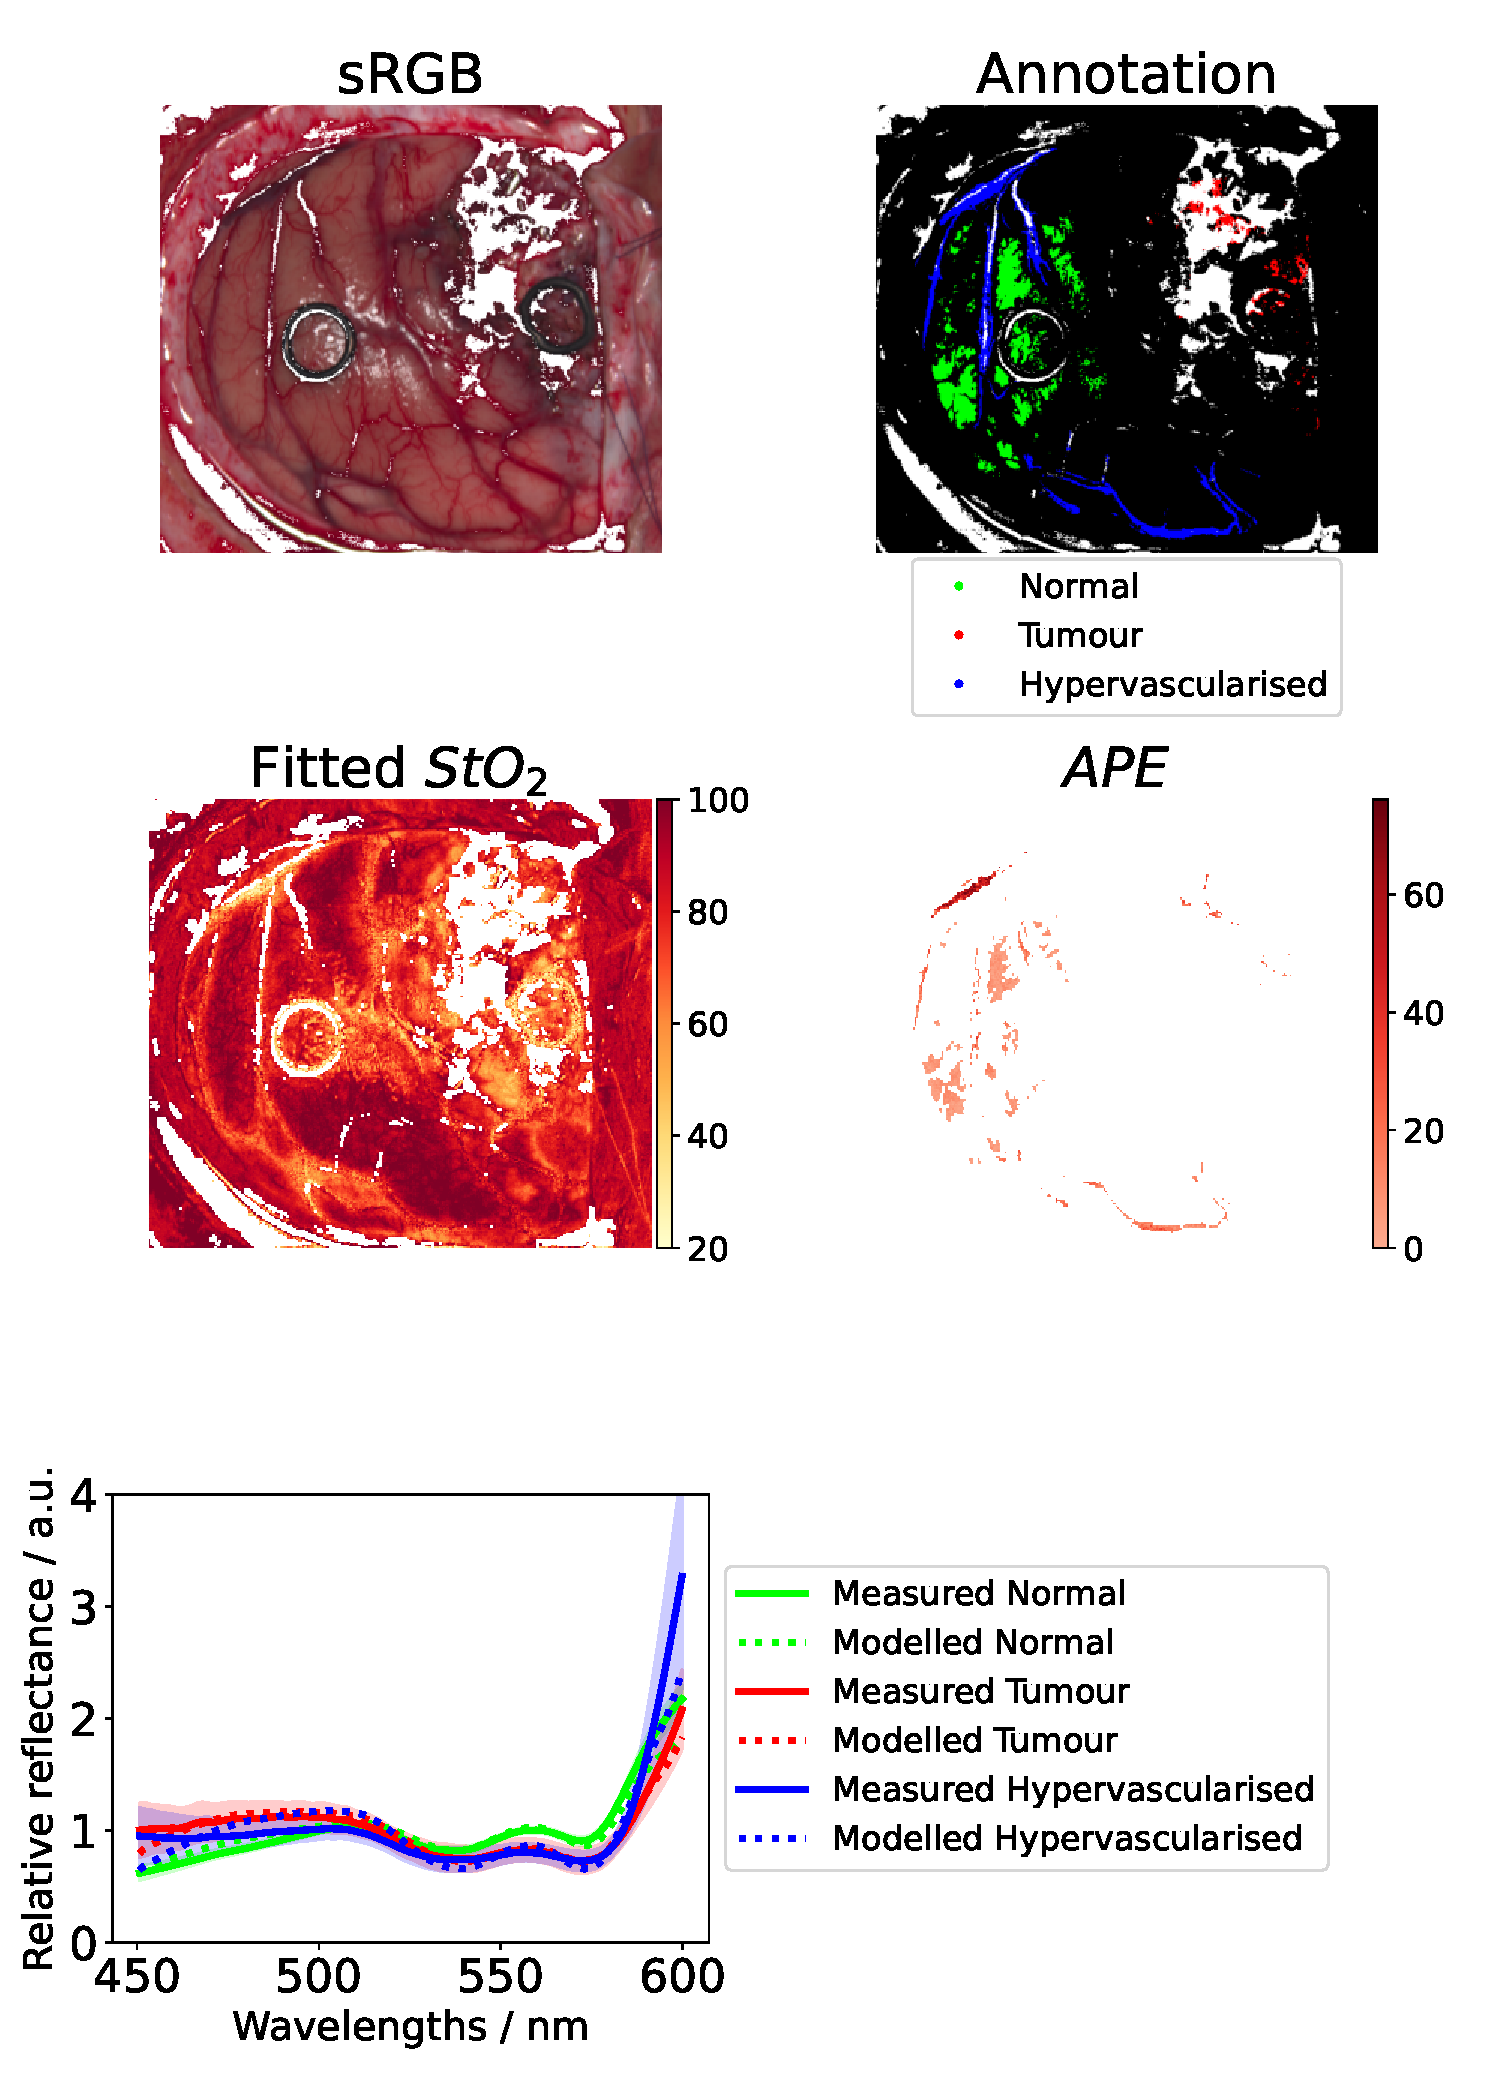
\includegraphics[width=\textwidth]{012-02_StO2_Y.pdf}
    \caption{Top left shows an sRGB reconstruction of the HELICoiD image 012-02 with the regions beyond thresholds shown as white. Top right shows an annotation of the same image. Middle left shows the fitted $StO_2$ on a pixel-by-pixel basis using the Yudovsky 2009 single-layer model and shifted extinction coefficients. Middle right shows the $APE$ of the fitted $StO_2$ of each pixel in each annotated region compared to the fitted $StO_2$ from the mean spectrum of the annotated region, however this is only computed in the annotated regions. Bottom shows the mean annotated spectra of each tissue type ($\pm$ standard deviation) plotted with the modelled spectra using parameters fitted to the mean annotated spectrum.}
    \label{fig:HELICoiDpixelY}
\end{figure}

\FloatBarrier
\section{Discussion} \label{sec:discussion5}
When simulating camera responses from Monte Carlo data and the analytical models, there remains very high similarity (as shown by the $NRMSE$ and $r$) when there is no simulated noise. This confirms the expectation that using the same camera simulation for the forwards models and the Monte Carlo data, results in the similarity of these spectra being retained. When the noise is increased for the Monte Carlo camera response simulation the similarity to the noiseless model-predicted reflectance decreases. Both Yudovsky 2009 and Jacques 1999 single-layer models behave similarly with little difference in correlation between modelled and simulated spectra as noise is increased, however the Yudovsky 2009 double-layer model shows more significant correlation reduction. For all models investigated, mean normalising the data results in poorer correlation with this reduction being more prominent for Yudovsky 2009 double-layer model. This reduction in correlation when noise is increased is expected, however the double-layer model appears more susceptible to the impact of this than the single-layer models. 

By fitting the models to Monte Carlo simulations with simulated camera responses and varying noise levels, the inverse problem is investigated. This shows the quality of parameter extraction rapidly decrease on increase in noise for every parameter and model with the double-layer model showing a more pronounced effect than the single-layer models, confirming that this model is more sensitive to noise. In the event of no noise being present, the Yudovsky 2009 and Jacques 1999 single-layer models both show excellent parameter extraction for all physiological parameters for quantitative data which is retained for $StO_2$ and $b$ for relative data. When noise is introduced, however, the quality of parameter extraction is significantly reduced with the precision of the recovered parameters reduced even where their trend remains relatively preserved. This is markedly worse when relative data is used. This demonstrates the importance of noise reduction methods in HSI data acquisition in order to obtain accurate parameter extraction, particularly when relative data is used. 

When simulating the camera response for the forwards single-layer models or the spectrophotometer measurements compared to the mean annotated spectrum from HSI snapshot frames of the gelatin-based phantoms, the correlation of the spectra remain high (as shown by $r$), however the absolute errors increase in comparison to Table \ref{tb:NRMSEphantom}. This can be seen by slight changes in all camera simulated spectra from the mean annotated spectra, most notably in the 525-575nm region where $StO_2$ or $AR1$ has a large impact on the spectral shape. This demonstrates that the simple approach to camera simulation may require improvement. In these statistics, only bands with central wavelengths less than 575nm are considered since Chapter \ref{chap:1layer} shows poor performance of the models beyond this meaning only 13 bands are used. The impact of this poor performance, however, may not be fully eliminated as bands with lower central wavelengths may be sensitive to wavelengths above 575nm due to cross-talk effects seen in Figure \ref{fig:bandresponses}, however this should then be corrected using the correction matrix. This would, however, not be problematic in the spectrophotometer response suggesting there are also other factors impacting the poorer camera simulation. 

Fitting the single-layer models to the mean annotated spectrum of each gelatin-based phantom, shows the quality of parameter extraction is overall lower than when fitting to spectrophotometer responses as in Table \ref{tb:phantomparams}. Similar to the results of fitting to spectrophotometer responses, only $AR1$ and $AR14$ are extracted well, with $c_{tot}$ and $I$ very poorly recovered so only the former are discussed. Yudovsky 2009 recovers these parameters with better quality than Jacques 1999 in all cases, however the use of relative data dramatically increases the mean $APE$ despite preserving the overall trends demonstrating an offset compared to the ground-truth values. This is likely to reflect the flawed camera simulation used in fitting to these spectra which is mismatched in regions where the dyes have significant impact. When fitting, instead, to each pixel spectrum of the annotated regions it can be seen that the errors follow similar trends but are inflated when using a single, likely due to noise which is present in this regime but largely removed when the mean spectrum is taken or when the mean of 5 frames is used. Whilst some trends and mean $APE$ are relatively well preserved, the precision of the parameter recovery is sacrificed when a single frame is analysed pixelwise due to the increased noise. For this reason, it is clear that effective denoising strategies are necessary to obtain high quality results. 

When fitting to HELICoiD neurosurgical linescan HSI relative mean annotated spectra, it is noticeable that the literature Haemoglobin peaks appear offset from those measured. When shifting these peaks by 3nm they appear more in line with the mean annotated spectra, suggesting that the wavelength calibration of this data may not be fully accurate or the environment of the haemoglobin is impacting its absorption spectra as seen for the dyes used in Chapter \ref{chap:1layer}. It is also noted that the spectrum forms a closer fit to the region of the spectrum associated most strongly with Hemoglobin when this region is weighted in the residual. There appears to be some decrease in mean fitted $StO_2$ as fitting is improved to this region of the spectrum, however the distribution of values appears very similar and lower than those considered typical by JVOS or cerebral oximetry for all methods tested. This demonstrates the importance of accurate optical modelling of the tissue for quality parameter extraction. 
%These methods are also applied with a simulated camera response to relative mean annotated NeuroHSI neurosurgical snapshot HSI data. This reduction in bands and introduction of simulated camera response returns very poor parameter extraction, despite excellent visual fits to the spectra. This may be linked to the poor camera simulation in the region of largest $StO_2$ impact (525-575nm) as seen with the gelatin-based phantoms. 

Finally, the Yudovsky 2009 single-layer model is applied using the shifted extinction coefficients to an exemplary HELICoiD image (012-02) on a pixel-by-pixel basis. This results in an $StO_2$ image demonstrating difference between tissues and vessels with spatial resolution. This may demonstrate potential for this technology in future work, however there are no ground truth values here with which to evaluate the success of this analysis.

\subsection{Limitations}
The most notable limitation of this work is the computational time associated as pixel-by-pixel analysis taking many hours per image using the current implementation. This would not be feasible in a clinical environment and limits the use of this technology. 

Other limitations (as mentioned in Section \ref{sec:discussion5}) include possibility of the poorer regions of model prediction to be impacting the more successful regions when modelling gelatin-based phantoms due to cross-talk between snapshot bands, the need for further validation of the optical characterisation of tissues, and unknown ground truth values of $StO_2$ for these tissues and images for rigorous evaluation. Another limitation is that, whilst temporal averaging provided significant improvement of the results shown for the static videos of gelatin-based phantoms, the use of temporal averaging in surgical videos would likely result in motion artefacts thus suggesting that improved noise reduction methods should be investigated. 

Additionally, whilst the HELICoiD dataset is able to provide high spectral resolution neurosurgical HSI images, the associated annotations only determine a small number of classes. This results in limited distinction between regions expected to have large variation in $StO_2$, such as arterial or venous vessels. This may result in unusual mean annotated spectra which aggregate these tissue types. These annotations also make use of SAM which results in only pixels of the same tissue with high spectral similarity being annotated, while there may be pixels of the same class with greater variation that are not included. This may result in artificially low variation in the spectrum of each class which may then not capture the full variety of spectra associated with that tissue type. This may result in fitted parameters on a pixel-by-pixel level showing larger variation from the annotated values for both the reasons that the class encompasses multiple sub-types of tissue, and that the mean spectrum may not encompass the full variation in the spectrum of each tissue type which may be captured by the manual annotation of a clinician. % as in the NeuroHSI dataset. 

Further to this point, these models should be tested on neurosurgical data taken with a similar configuration to that used for the phantom analysis with sufficient denoising performed. 

Finally, only single-layer models are used to analyse these neurosurgical datasets, however it is clear that Arachnoid or Pia Mater tissues may be present in a layered manner here. Arachnoid is known to show some absorbance, whereas Pia Mater is known to contain significant collagen which would indicate a likely scattering effect~\citep{Ghannam2023}. Whilst these layers usually have low thickness~\citep{Ghannam2023}, these effects may impact the diffuse reflectance spectrum measured and so two-layer modelling may be necessary to fully capture this. 

\subsection{Conclusion and future work}
In conclusion, this chapter shows that these models are able to obtain good quality results from quantitative snapshot hyperspectral data using well-defined optical properties, despite some oversimplification in the camera simulation. Relative data, however should be used with more caution demonstating a much larger impact of this camera simulation. When applied to neurosurgical hyperspectral linescan data, quantitative evaluation is more challenging due to the lack of known ground truth values. From visual inspection of this data, it appears that further work must be done to validate the modelling of the optical properties of these tissues. There is, however, promise that with an increased prior knowledge, these models may be able to provide valuable clinical parameters. 

Future work should include improving the computation time to allow for faster processing. This could be done by parallelising the computation of pixels using GPU processing, or by training a deep-learning network using the forwards models to generate training data. The bands chosen for the snapshot mosaic camera should be optimised to be most informative on the optical properties and to minimise cross-talk. This should be informed by well-characterised optical properties of these tissues which should be investigated further. The algorithm established in Chapter \ref{chap:SWB} should be used in it's extensive version to obtain intra-operative, quantitative, snapshot data. This should be combined with denoising techniques that preserve the spatial, spectral, and temporal resolution of the data to allow the possibility of good quality parameter extraction in real-time. Finally, the two-layer model should be explored for improvement in quality and this should be used to account for the meninges of the brain when analysing neurosurgical data. 

\begin{subappendices}
    
\section{Appendices investigating simulated HSI camera data}
\begin{table}[bhp]
    \centering
    \caption{Mean ($\pm$ standard deviation) $NRMSE$ (3.d.p.) between the simulated camera responses of each forwards spectrum from each model and each of 100 Monte Carlo simulated spectra using the same ground truth variable parameters for each refractive index dataset for quantitative data at a variety of noise levels (0pp, 1pp, 3pp). This is presented with the Pearson $r$ (bold if Pearson $p < 0.05$) for the linear regression between all forwards spectra against Monte Carlo simulated spectra for each refractive index dataset and each analytical model. All metrics are evaluated for the wavelength region of 450-600nm.}
    \begin{tabular}{|cc|c|ccc|ccc|}
        \hline
        Model & Layers & Refractive & \multicolumn{3}{|c}{$NRMSE$} & \multicolumn{3}{|c|}{$r$} \\
         & & index & 0pp & 1pp & 3pp & 0pp & 1pp & 3pp \\
        \hline
        \multirow{3}{*}{\shortstack{Yudovsky\\ 2009}} & \multirow{3}{*}{1} & 1.33 & \shortstack{0.012 \\($\pm$ 0.006)} & \shortstack{0.077 \\($\pm$ 0.054)} & \shortstack{0.204 \\($\pm$ 0.128)} & \textbf{1.000} & \textbf{0.996} & \textbf{0.959} \\
        & & 1.35 & \shortstack{0.011 \\($\pm$ 0.005)} & \shortstack{0.088 \\($\pm$ 0.063)} & \shortstack{0.241 \\($\pm$ 0.150)} & \textbf{1.000} & \textbf{0.993} & \textbf{0.944} \\
        & & 1.44 & \shortstack{0.009 \\($\pm$ 0.004)} & \shortstack{0.082 \\($\pm$ 0.057)} & \shortstack{0.224 \\($\pm$ 0.125)} & \textbf{1.000} & \textbf{0.993} & \textbf{0.942} \\
        \hline
        \multirow{3}{*}{\shortstack{Jacques\\ 1999}} & \multirow{3}{*}{1} & 1.33 & \shortstack{0.033 \\($\pm$ 0.063)} & \shortstack{0.086 \\($\pm$ 0.084)} & \shortstack{0.206 \\($\pm$ 0.137)} & \textbf{1.000} & \textbf{0.995} & \textbf{0.959} \\
        & & 1.35 & \shortstack{0.040 \\($\pm$ 0.071)} & \shortstack{0.100 \\($\pm$ 0.092)} & \shortstack{0.242 \\($\pm$ 0.153)} & \textbf{0.999} & \textbf{0.992} & \textbf{0.943} \\
        & & 1.44 & \shortstack{0.026 \\($\pm$ 0.046)} & \shortstack{0.089 \\($\pm$ 0.077)} & \shortstack{0.227 \\($\pm$ 0.130)} & \textbf{1.000} & \textbf{0.993} & \textbf{0.942} \\
        \hline
        \shortstack{Yudovsky\\ 2009} & 2 & 1.44 & \shortstack{0.166 \\($\pm$ 0.133)} & \shortstack{0.482 \\($\pm$ 0.289)} & \shortstack{0.738 \\($\pm$ 0.294)} & \textbf{0.992} & \textbf{0.971} & \textbf{0.829} \\
        \hline
    \end{tabular}
    \label{ap:forwardsHSIMCq}
\end{table}
\FloatBarrier

\begin{table}[bhp]
    \centering
    \caption{Mean ($\pm$ standard deviation) $NRMSE$ (3.d.p.) between the simulated camera responses of each forwards spectrum from each model and each of 100 Monte Carlo simulated spectra using the same ground truth variable parameters for each refractive index dataset for relative data at a variety of noise levels (0pp, 1pp, 3pp). This is presented with the Pearson $r$ (bold if Pearson $p < 0.05$) for the linear regression between all forwards spectra against Monte Carlo simulated spectra for each refractive index dataset and each analytical model. All metrics are evaluated for the wavelength region of 450-600nm.}
    \begin{tabular}{|cc|c|ccc|ccc|}
        \hline
        Model & Layers & Refractive & \multicolumn{3}{|c}{$NRMSE$} & \multicolumn{3}{|c|}{$r$} \\
         & & index & 0pp & 1pp & 3pp & 0pp & 1pp & 3pp \\
        \hline
        \multirow{3}{*}{\shortstack{Yudovsky\\ 2009}} & \multirow{3}{*}{1} & 1.33 & \shortstack{0.004 \\($\pm$ 0.003)} & \shortstack{0.071 \\($\pm$ 0.057)} & \shortstack{0.203 \\($\pm$ 0.142)} & \textbf{1.000} & \textbf{0.908} & \textbf{0.559} \\
        & & 1.35 & \shortstack{0.003 \\($\pm$ 0.003)} & \shortstack{0.085 \\($\pm$ 0.063)} & \shortstack{0.237 \\($\pm$ 0.150)} & \textbf{1.000} & \textbf{0.886} & \textbf{0.530} \\
        & & 1.44 & \shortstack{0.003 \\($\pm$ 0.002)} & \shortstack{0.075 \\($\pm$ 0.044)} & \shortstack{0.212 \\($\pm$ 0.118)} & \textbf{1.000} & \textbf{0.916} & \textbf{0.602} \\
        \hline
        \multirow{3}{*}{\shortstack{Jacques\\ 1999}} & \multirow{3}{*}{1} & 1.33 & \shortstack{0.018 \\($\pm$ 0.026)} & \shortstack{0.073 \\($\pm$ 0.062)} & \shortstack{0.204 \\($\pm$ 0.144)} & \textbf{0.992} & \textbf{0.899} & \textbf{0.545} \\
        & & 1.35 & \shortstack{0.021 \\($\pm$ 0.029)} & \shortstack{0.087 \\($\pm$ 0.064)} & \shortstack{0.239 \\($\pm$ 0.152)} & \textbf{0.990} & \textbf{0.884} & \textbf{0.519} \\
        & & 1.44 & \shortstack{0.014 \\($\pm$ 0.021)} & \shortstack{0.076 \\($\pm$ 0.045)} & \shortstack{0.212 \\($\pm$ 0.117)} & \textbf{0.995} & \textbf{0.915} & \textbf{0.605} \\
        \hline
        \shortstack{Yudovsky\\ 2009} & 2 & 1.44 & \shortstack{0.033 \\($\pm$ 0.026)} & \shortstack{0.428 \\($\pm$ 0.286)} & \shortstack{0.684 \\($\pm$ 0.286)} & \textbf{0.991} & \textbf{0.270} & -0.007 \\
        \hline
    \end{tabular}
    \label{ap:forwardsHSIMCr}
\end{table}
\FloatBarrier

\begin{table}[htb!]
    \centering
    \caption{The Pearson $r$ values (bold if $p<0.05$) of the linear regression line between the fitted tissue parameters and their ground truth displayed with their median (inter-quartile range) absolute percentage errors. This is shown for each variable and for each refractive index dataset when extracted by fitting Yudovsky 2009 single layer (Y1), Jacques 1999 (J), or Yudovsky 2009 double layer (Y2) to the quantitative Monte-Carlo datasets at each noise level (0pp, 1pp, 3pp). All presented to 3s.f.}
    \begin{tabular}{|ccc|ccc|ccc|}
        \hline
        Parameter & Model & Refractive & \multicolumn{3}{c}{$r$} & \multicolumn{3}{|c|}{median (inter-quartile range)} \\
        & & index & \multicolumn{3}{c}{} & \multicolumn{3}{|c|}{absolute percentage error (\%)} \\
        & & & 0pp & 1pp & 3pp & 0pp & 1pp & 3pp \\
        \hline
        \multirow{7}{*}{$StO_2$} & \multirow{3}{*}{Y1} & 1.33 & \textbf{0.999} & \textbf{0.794} & \textbf{0.403} & 2.25 (5.70) & 40.2 (74.5) & 79.5 (75.6) \\
        & & 1.35 & \textbf{0.999} & \textbf{0.668} & \textbf{0.628} & 1.41 (3.91) & 29.4 (27.4) & 54.4 (79.3) \\
        & & 1.44 & \textbf{0.999} & \textbf{0.825} & \textbf{0.369} & 1.90 (2.83) & 24.8 (60.7) & 85.2 (69.9) \\
        \cline{2-9}
        & \multirow{3}{*}{J} & 1.33 & \textbf{0.967} & \textbf{0.797} & \textbf{0.435} & 5.28 (19.1) & 30.7 (59.3) & 83.1 (71.2) \\
        & & 1.35 & \textbf{0.962} & \textbf{0.807} & \textbf{0.629} & 4.57 (24.0) & 31.2 (64.4) & 51.4 (81.4) \\
        & & 1.44 &  \textbf{0.978} & \textbf{0.829} & \textbf{0.402} & 4.06 (11.3) & 22.5 (60.8) & 83.6 (77.7) \\
        \cline{2-9}
        & Y2 & 1.44 & \textbf{0.751} & 0.0612 & 0.0194 & 16.8 (25.5) & 66.5 (51.5) & 68.9 (55.3) \\
        \hline
        \multirow{7}{*}{$f_{blood}$} & \multirow{3}{*}{Y1} & 1.33 & \textbf{0.980} & \textbf{0.743} & \textbf{0.552} & 2.25 (5.70) & 27.1 (33.7) & 45.7 (43.5) \\
        & & 1.35 & \textbf{0.974} & \textbf{0.668} & \textbf{0.386} & 4.26 (7.53) & 29.4 (27.4) & 51.6 (52.5) \\
        & & 1.44 & \textbf{0.984} & \textbf{0.667} & \textbf{0.450} & 5.83 (6.97) & 23.7 (38.9) & 51.8 (44.3)\\
        \cline{2-9}
        & \multirow{3}{*}{J} & 1.33 & \textbf{0.918} & \textbf{0.768} & \textbf{0.604} & 8.68 (23.6) & 26.6 (35.3) & 42.6 (49.4) \\
        & & 1.35 & \textbf{0.912} & \textbf{0.736} & \textbf{0.432} & 11.3 (18.8) & 27.7 (34.8) & 48.2 (45.9) \\
        & & 1.44 & \textbf{0.924} & \textbf{0.719} & \textbf{0.498} & 7.14 (15.9) & 25.0 (39.4) & 46.7 (42.4) \\
        \cline{2-9}
        & Y2 & 1.44 & \textbf{0.872} & 0.147 & 0.0329 & 23.1 (25.4) & 115 (197) & 160 (291) \\
        \hline
        \multirow{7}{*}{$a$} & \multirow{3}{*}{Y1} & 1.33 & \textbf{0.993} & \textbf{0.828} & \textbf{0.677} & 5.34 (6.11) & 19.1 (25.1) & 29.0 (40.5) \\
        & & 1.35 & \textbf{0.995} & \textbf{0.824} & \textbf{0.627} & 3.61 (5.95) & 20.0 (25.5) & 36.7 (39.7) \\
        & & 1.44 & \textbf{0.992} & \textbf{0.773} & \textbf{0.558} & 3.85 (5.16) & 18.7 (34.7) & 35.1 (39.1) \\
        \cline{2-9}
        & \multirow{3}{*}{J} & 1.33 & \textbf{0.955} & \textbf{0.817} & \textbf{0.682} & 6.33 (20.5) & 19.5 (25.3) & 25.9 (37.6) \\
        & & 1.35 & \textbf{0.968} & \textbf{0.815} & \textbf{0.641} & 8.47 (17.0) & 20.0 (26.4) & 37.1 (38.6) \\
        & & 1.44 & \textbf{0.961} & \textbf{0.759} & \textbf{0.542} & 4.69 (14.0) & 17.1 (31.8) & 30.4 (39.9) \\
        \cline{2-9}
        & Y2 & 1.44 & \textbf{0.674} & 0.00365 & 0.0666 & 17.9 (13.8) & 37.8 (26.8) & 37.4 (26.1) \\
        \hline
        \multirow{9}{*}{$b$} & \multirow{3}{*}{Y1} & 1.33 & \textbf{0.996} & \textbf{0.689} & \textbf{0.370} & 2.28 (3.17) & 25.4 (54.9) & 55.5 (72.2) \\
        & & 1.35 & \textbf{0.996} & \textbf{0.682} & \textbf{0.426} & 2.24 (3.94) & 36.0 (75.1) & 58.2 (69.6) \\
        & & 1.44 & \textbf{0.998} & \textbf{0.751} & \textbf{0.516} & 2.63 (3.63) & 21.8 (46.8) & 52.0 (68.3) \\
        \cline{2-9}
        & \multirow{3}{*}{J} & 1.33 & \textbf{0.874} & \textbf{0.679} & \textbf{0.410} & 5.13 (12.8) & 30.0 (54.0) & 58.0 (74.6) \\
        & & 1.35 & \textbf{0.838} & \textbf{0.646} & \textbf{0.446} & 6.22 (34.2) & 40.4 (74.2) & 57.8 (71.4) \\
        & & 1.44 & \textbf{0.934} & \textbf{0.757} & \textbf{0.515} & 5.70 (16.5) & 23.7 (52.9) & 50.4 (71.4) \\
        \cline{2-9}
        & Y2 & 1.44 & \textbf{0.735} & 0.169 & -0.00249 & 16.8 (19.3) & 56.4 (48.2) & 61.3 (54.9) \\
        \hline
        $f_mel$ & Y2 & 1.44 & \textbf{0.852} & \textbf{0.622} & \textbf{0.477} & 28.0 (31.7) & 85.1 (128) & 90.1 (120) \\
        \hline
        $L_1$ & Y2 & 1.44 & \textbf{0.824} & \textbf{0.401} & 0.123 & 36.7 (40.9) & 69.5 (83.1) & 84.5 (96.0) \\
        \hline
    \end{tabular}    
    \label{ap:backwardsHSIMCq}
\end{table}

\begin{table}[htb!]
    \centering
    \caption{The Pearson $r$ values (bold if $p<0.05$) of the linear regression line between the fitted tissue parameters and their ground truth displayed with their median (inter-quartile range) absolute percentage errors. This is shown for each variable and for each refractive index dataset when extracted by fitting Yudovsky 2009 single layer (Y1), Jacques 1999 (J), or Yudovsky 2009 double layer (Y2) to the relative Monte-Carlo datasets at each noise level (0pp, 1pp, 3pp). All presented to 3s.f.}
    \begin{tabular}{|ccc|ccc|ccc|}
        \hline
        Parameter & Model & Refractive & \multicolumn{3}{c}{$r$} & \multicolumn{3}{|c|}{median (inter-quartile range)} \\
        & & index & \multicolumn{3}{c}{} & \multicolumn{3}{|c|}{absolute percentage error (\%)} \\
        & & & 0pp & 1pp & 3pp & 0pp & 1pp & 3pp \\
        \hline
        \multirow{7}{*}{$StO_2$} & \multirow{3}{*}{Y1} & 1.33 & \textbf{0.999} & \textbf{0.799} & \textbf{0.420} & 2.32 (5.27) & 28.3 (74.8) & 65.1 (70.9) \\
        & & 1.35 & \textbf{0.998} & \textbf{0.741} & \textbf{0.550} & 1.92 (2.93) & 40.6 (46.1) & 45.0 (77.2) \\
        & & 1.44 & \textbf{0.999} & \textbf{0.752} & \textbf{0.410} & 2.23 (3.06) & 41.4 (81.1) & 76.7 (77.6) \\
        \cline{2-9}
        & \multirow{3}{*}{J} & 1.33 & \textbf{0.968} & \textbf{0.809} & \textbf{0.444} & 6.44 (17.5) & 31.3 (55.6) & 64.3 (73.7) \\
        & & 1.35 & \textbf{0.959} & \textbf{0.758} & \textbf{0.568} & 4.41 (21.1) & 37.0 (51.8) & 59.6 (77.5) \\
        & & 1.44 &  \textbf{0.977} & \textbf{0.755} & \textbf{0.447} & 4.77 (10.3) & 40.3 (82.5) & 76.7 (77.6) \\
        \cline{2-9}
        & Y2 & 1.44 & \textbf{0.679} & \textbf{0.198} & 0.0448 & 18.8 (30.9) & 63.0 (45.6) & 75.1 (62.5) \\
        \hline
        \multirow{7}{*}{$f_{blood}$} & \multirow{3}{*}{Y1} & 1.33 & \textbf{0.851} & \textbf{0.584} & \textbf{0.653} & 16.5 (27.3) & 36.3 (49.2) & 56.7 (42.7) \\
        & & 1.35 & \textbf{0.840} & \textbf{0.579} & \textbf{0.328} & 16.0 (22.1) & 46.9 (47.2) & 59.6 (50.8) \\
        & & 1.44 & \textbf{0.870} & \textbf{0.547} & \textbf{0.535} & 16.7 (23.9) & 47.5 (40.1) & 51.1 (42.7)\\
        \cline{2-9}
        & \multirow{3}{*}{J} & 1.33 & \textbf{0.854} & \textbf{0.707} & \textbf{0.723} & 24.2 (36.4) & 30.6 (47.2) & 47.1 (45.5) \\
        & & 1.35 & \textbf{0.836} & \textbf{0.727} & \textbf{0.386} & 20.3 (28.7) & 34.6 (47.0) & 55.1 (60.6) \\
        & & 1.44 & \textbf{0.859} & \textbf{0.681} & \textbf{0.644} & 24.1 (28.5) & 39.6 (50.6) & 45.0 (52.0) \\
        \cline{2-9}
        & Y2 & 1.44 & \textbf{0.609} & 0.189 & 0.0466 & 37.6 (56.2) & 97.7 (142) & 108 (152) \\
        \hline
        \multirow{7}{*}{$a$} & \multirow{3}{*}{Y1} & 1.33 & \textbf{0.695} & \textbf{0.213} & 0.181 & 23.0 (32.6) & 44.5 (60.6) & 71.1 (44.9) \\
        & & 1.35 & \textbf{0.774} & \textbf{0.213} & 0.0827 & 21.8 (29.6) & 60.9 (61.3) & 66.2 (54.2) \\
        & & 1.44 & \textbf{0.703} & 0.160 & \textbf{0.558} & 26.2 (29.5) & 62.3 (53.7) & 35.1 (39.1) \\
        \cline{2-9}
        & \multirow{3}{*}{J} & 1.33 & \textbf{0.524} & \textbf{0.493} & 0.144 & 29.2 (49.5) & 38.2 (60.8) & 56.9 (54.6) \\
        & & 1.35 & \textbf{0.677} & \textbf{0.261} & 0.00248 & 30.3 (52.5) & 45.7 (56.1) & 61.0 (60.6) \\
        & & 1.44 & \textbf{0.431} & -0.00356 & 0.166 & 27.7 (44.1) & 57.7 (58.9) & 51.7 (53.1) \\
        \cline{2-9}
        & Y2 & 1.44 & \textbf{0.333} & 0.0199 & -0.100 & 27.0 (24.6) & 36.7 (21.4) & 42.2 (28.7) \\
        \hline
        \multirow{9}{*}{$b$} & \multirow{3}{*}{Y1} & 1.33 & \textbf{0.993} & \textbf{0.633} & \textbf{0.380} & 3.66 (6.61) & 34.6 (50.6) & 65.1 (69.8) \\
        & & 1.35 & \textbf{0.992} & \textbf{0.591} & \textbf{0.426} & 3.38 (6.76) & 44.1 (67.5) & 58.2 (69.6) \\
        & & 1.44 & \textbf{0.996} & \textbf{0.607} & \textbf{0.426} & 3.31 (8.11) & 39.5 (60.6) & 51.2 (73.8) \\
        \cline{2-9}
        & \multirow{3}{*}{J} & 1.33 & \textbf{0.893} & \textbf{0.634} & \textbf{0.325} & 7.18 (22.1) & 34.3 (57.1) & 54.9 (70.5) \\
        & & 1.35 & \textbf{0.850} & \textbf{0.579} & \textbf{0.374} & 11.4 (29.4) & 53.4 (67.4) & 61.6 (72.8) \\
        & & 1.44 & \textbf{0.938} & \textbf{0.641} & \textbf{0.441} & 7.66 (16.6) & 32.6 (60.5) & 46.4 (76.5) \\
        \cline{2-9}
        & Y2 & 1.44 & \textbf{0.360} & 0.0441 & -0.0711 & 33.2 (34.3) & 61.7 (50.2) & 63.6 (47.3) \\
        \hline
        $f_mel$ & Y2 & 1.44 & \textbf{0.517} & 0.166 & \textbf{0.201} & 35.3 (26.4) & 108 (119) & 132 (210) \\
        \hline
        $L_1$ & Y2 & 1.44 & \textbf{0.806} & 0.0777 & -0.0675 & 38.1 (37.0) & 65.4 (54.8) & 76.6 (86.8) \\
        \hline
    \end{tabular}    
    \label{ap:backwardsHSIMCr}
\end{table}
\FloatBarrier
\section{Appendices analysing HSI data examples}\label{ap:MoreHSIPhantomEgs}
\subsection{Using a single frame}
\begin{figure}[h!]
    \centering 
    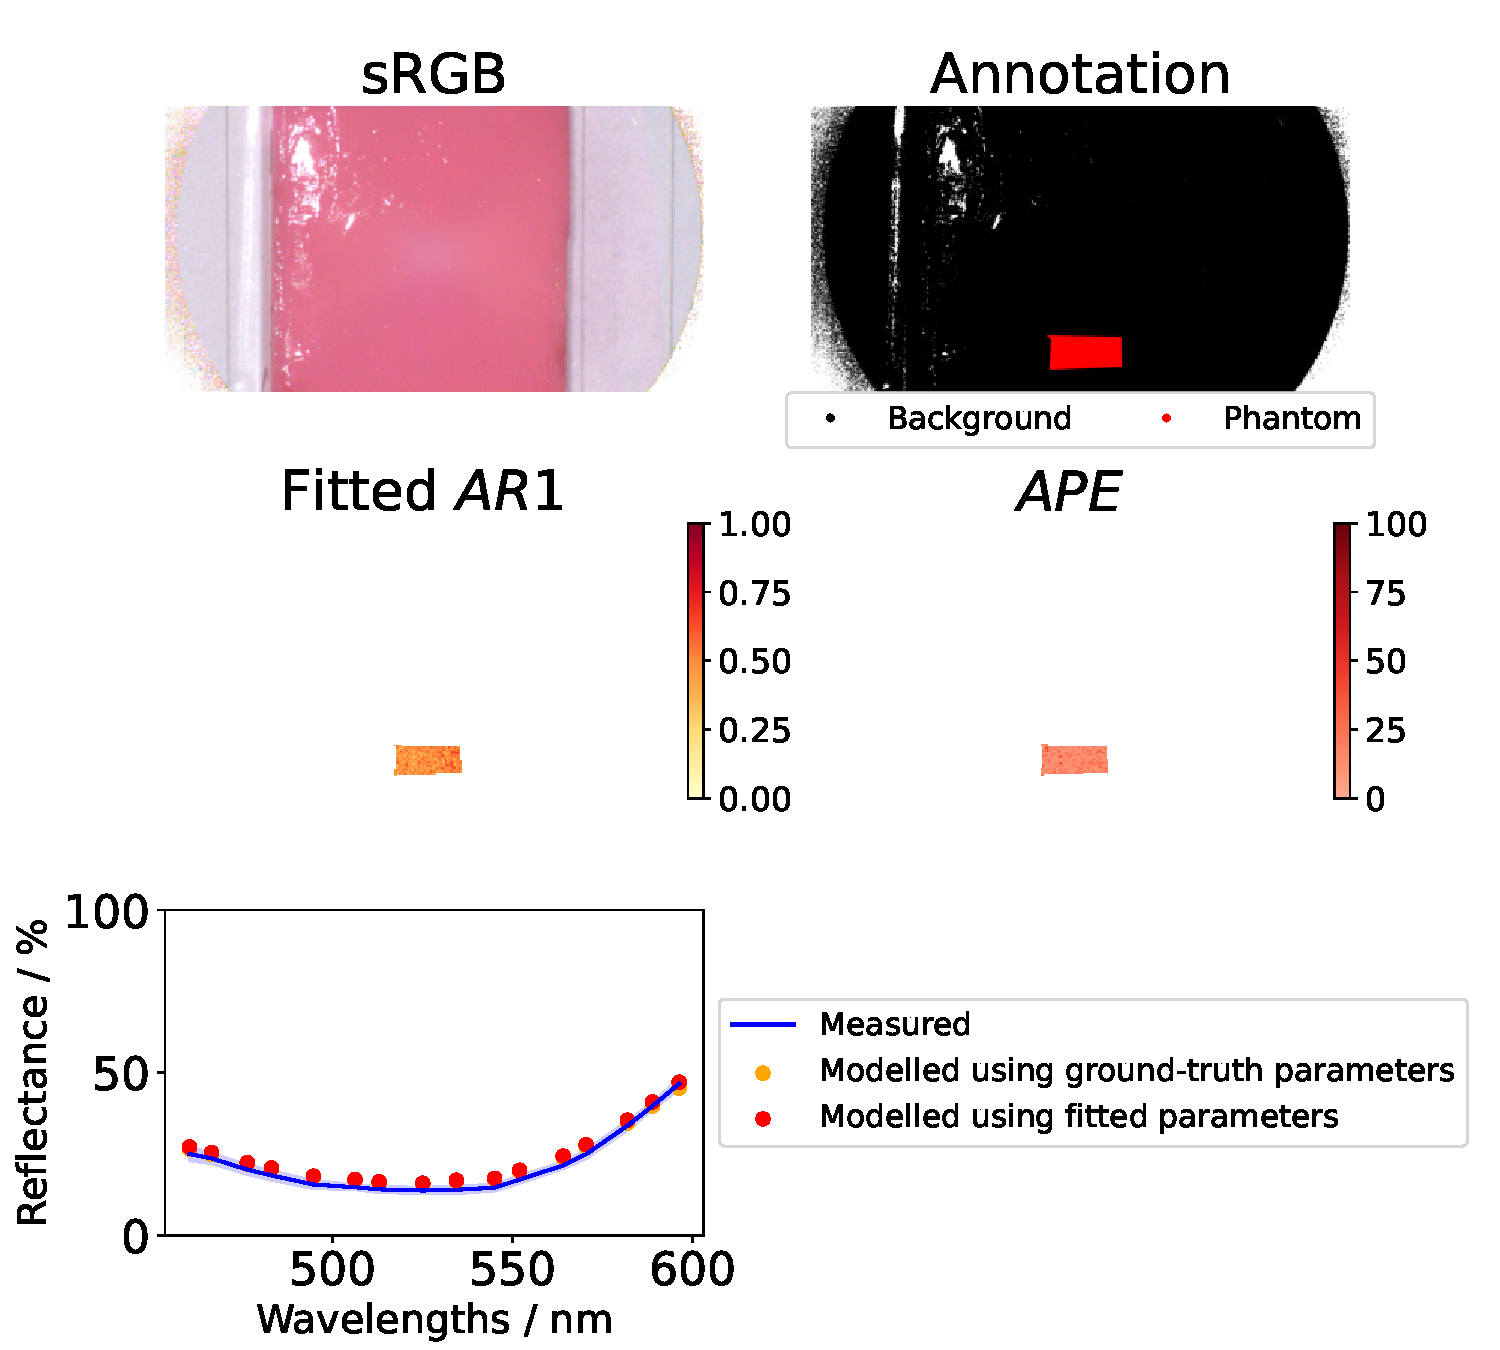
\includegraphics[width=\textwidth]{7_350_Y_OFF_AR1.pdf}
    \caption{Top left shows an sRGB reconstruction of a frame of a hyperspectral video of a gelatin-based phantom where $AR1=0.5$ and $I=3.50\%$ taken with a snapshot HSI camera, where the regions beyond thresholds are shown as white. Top right shows an annotation of the same image. Middle left shows the fitted $StO_2$ on a pixel-by-pixel basis of the quantitative data using the Yudovsky 2009 single-layer model. Middle right shows the $APE$ of the fitted $AR1$ of each pixel in the annotated region compared to the ground truth value (0.5). Bottom shows the mean annotated spectrum ($\pm$ standard deviation) plotted with the modelled spectrum using ground-truth parameters or parameters fitted to the mean annotated spectrum.}
    \label{ap:gelatinpbpegQY}
\end{figure}

\begin{figure}[h!]
    \centering 
    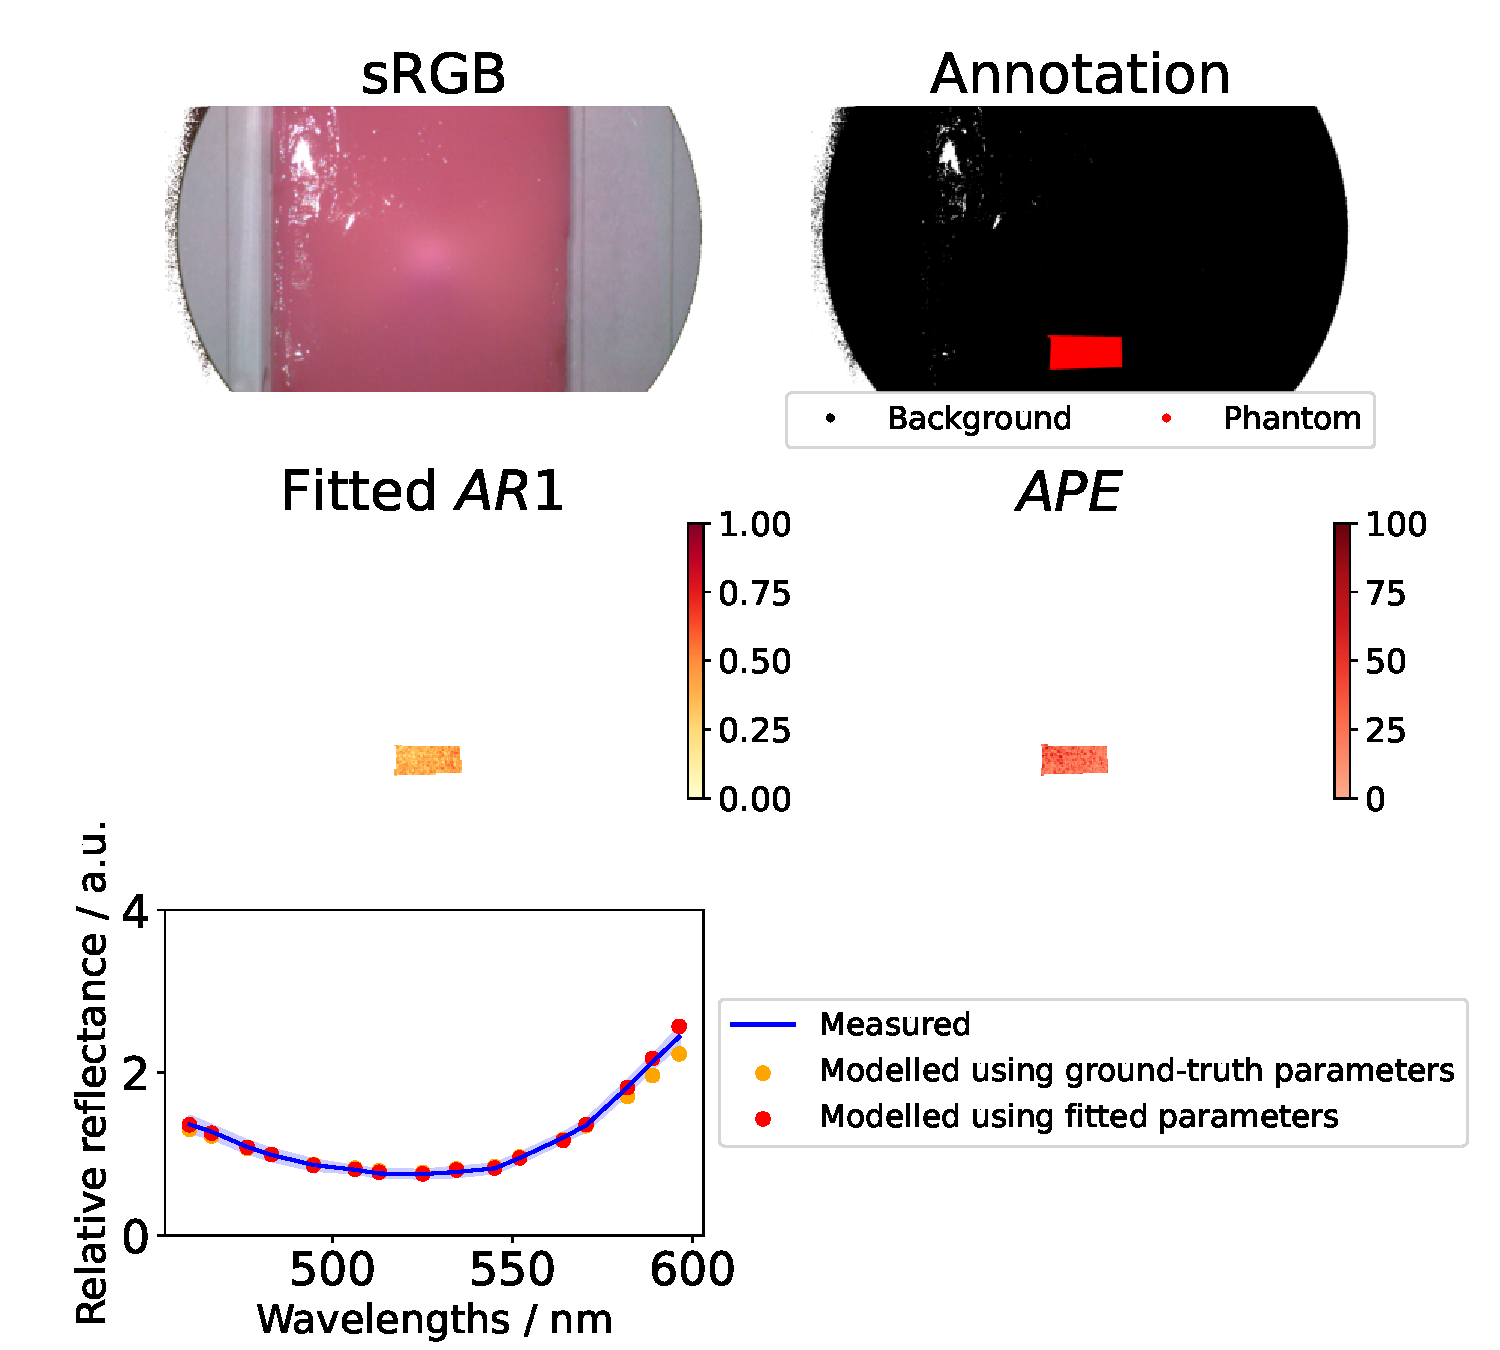
\includegraphics[width=\textwidth]{7_350_J_ON_AR1.pdf}
    \caption{Top left shows an sRGB reconstruction of a frame of a hyperspectral video of a gelatin-based phantom where $AR1=0.5$ and $I=3.50\%$ taken with a snapshot HSI camera, where the regions beyond thresholds are shown as white. Top right shows an annotation of the same image. Middle left shows the fitted $StO_2$ on a pixel-by-pixel basis of the relative data using the Jacques 1999 single-layer model. Middle right shows the $APE$ of the fitted $AR1$ of each pixel in the annotated region compared to the ground truth value (0.5). Bottom shows the mean annotated spectrum ($\pm$ standard deviation) plotted with the modelled spectrum using ground-truth parameters or parameters fitted to the mean annotated spectrum.}
    \label{ap:gelatinpbpegRJ}
\end{figure}

\begin{figure}[h!]
    \centering 
    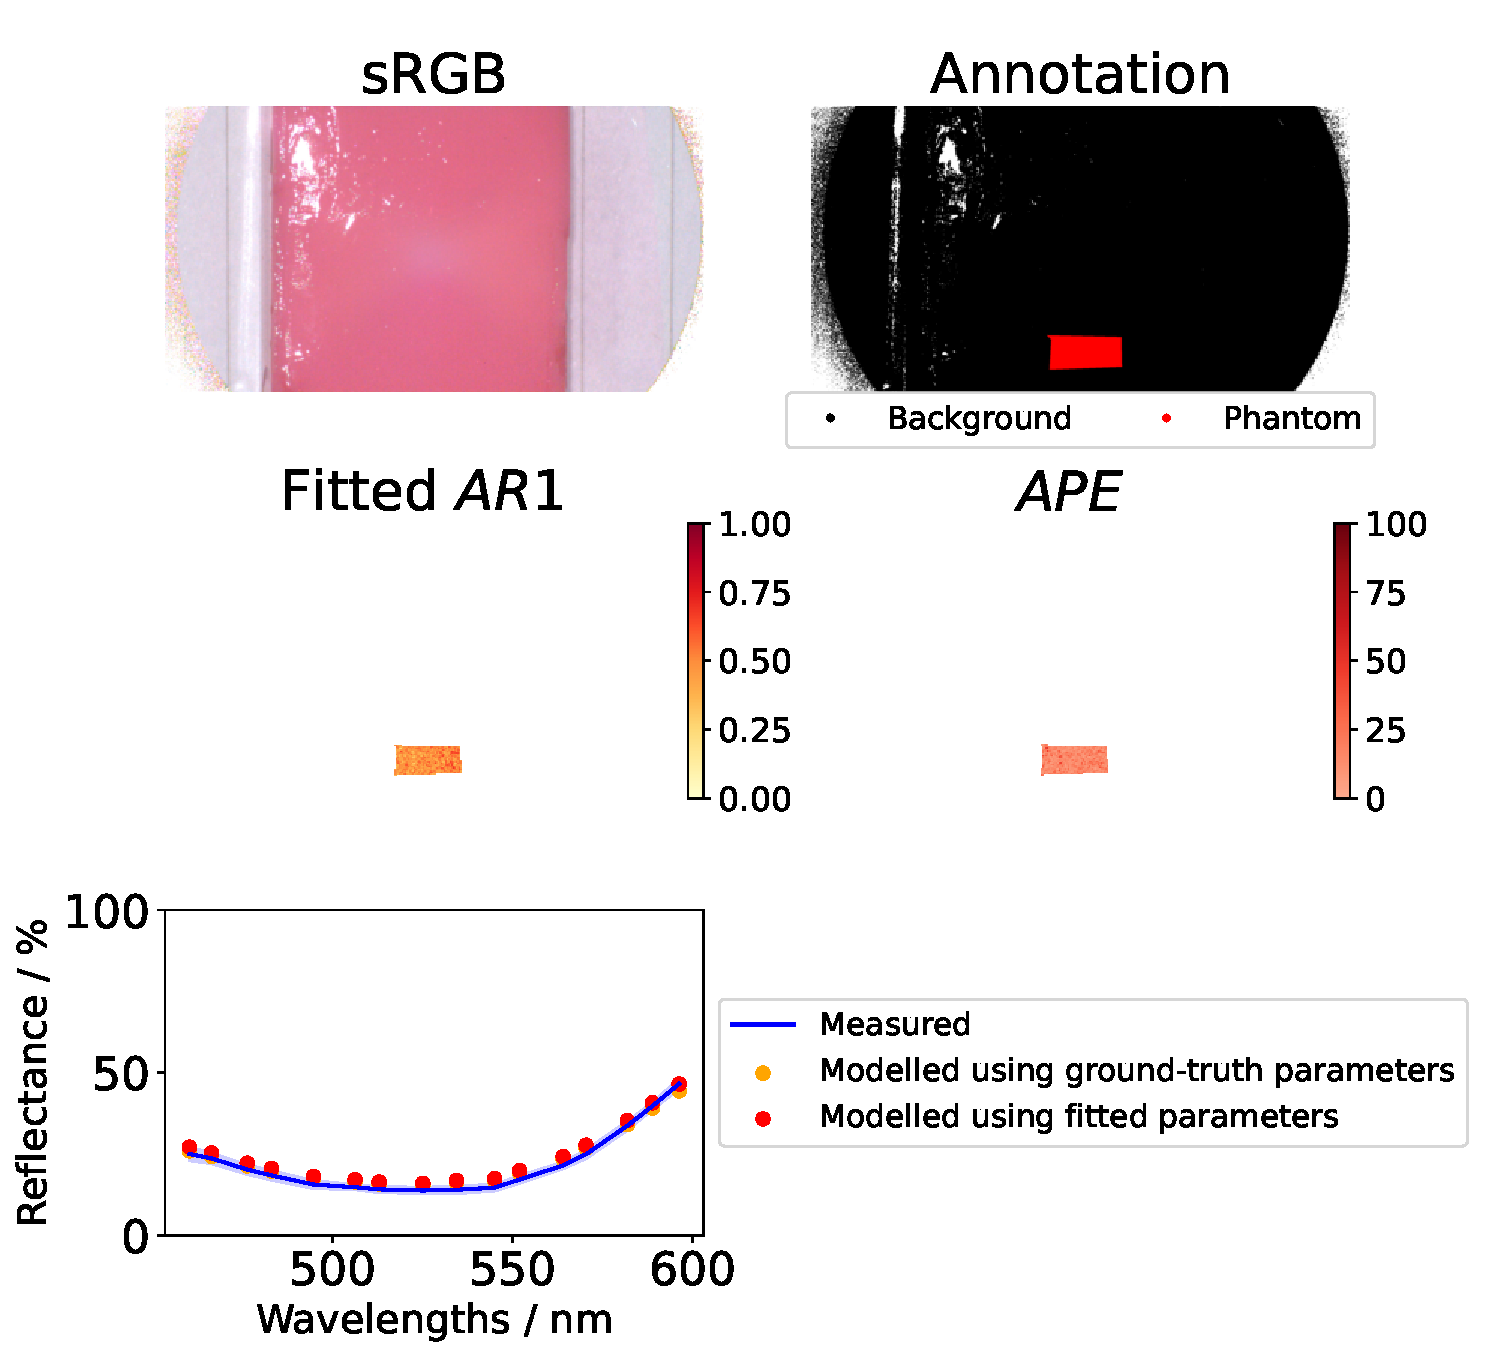
\includegraphics[width=\textwidth]{7_350_J_OFF_AR1.pdf}
    \caption{Top left shows an sRGB reconstruction of a frame of a hyperspectral video of a gelatin-based phantom where $AR1=0.5$ and $I=3.50\%$ taken with a snapshot HSI camera, where the regions beyond thresholds are shown as white. Top right shows an annotation of the same image. Middle left shows the fitted $StO_2$ on a pixel-by-pixel basis of the quantitative data using the Jacques 1999 single-layer model. Middle right shows the $APE$ of the fitted $AR1$ of each pixel in the annotated region compared to the ground truth value (0.5). Bottom shows the mean annotated spectrum ($\pm$ standard deviation) plotted with the modelled spectrum using ground-truth parameters or parameters fitted to the mean annotated spectrum.}
    \label{ap:gelatinpbpegQJ}
\end{figure}

\begin{figure}[h!]
    \centering 
    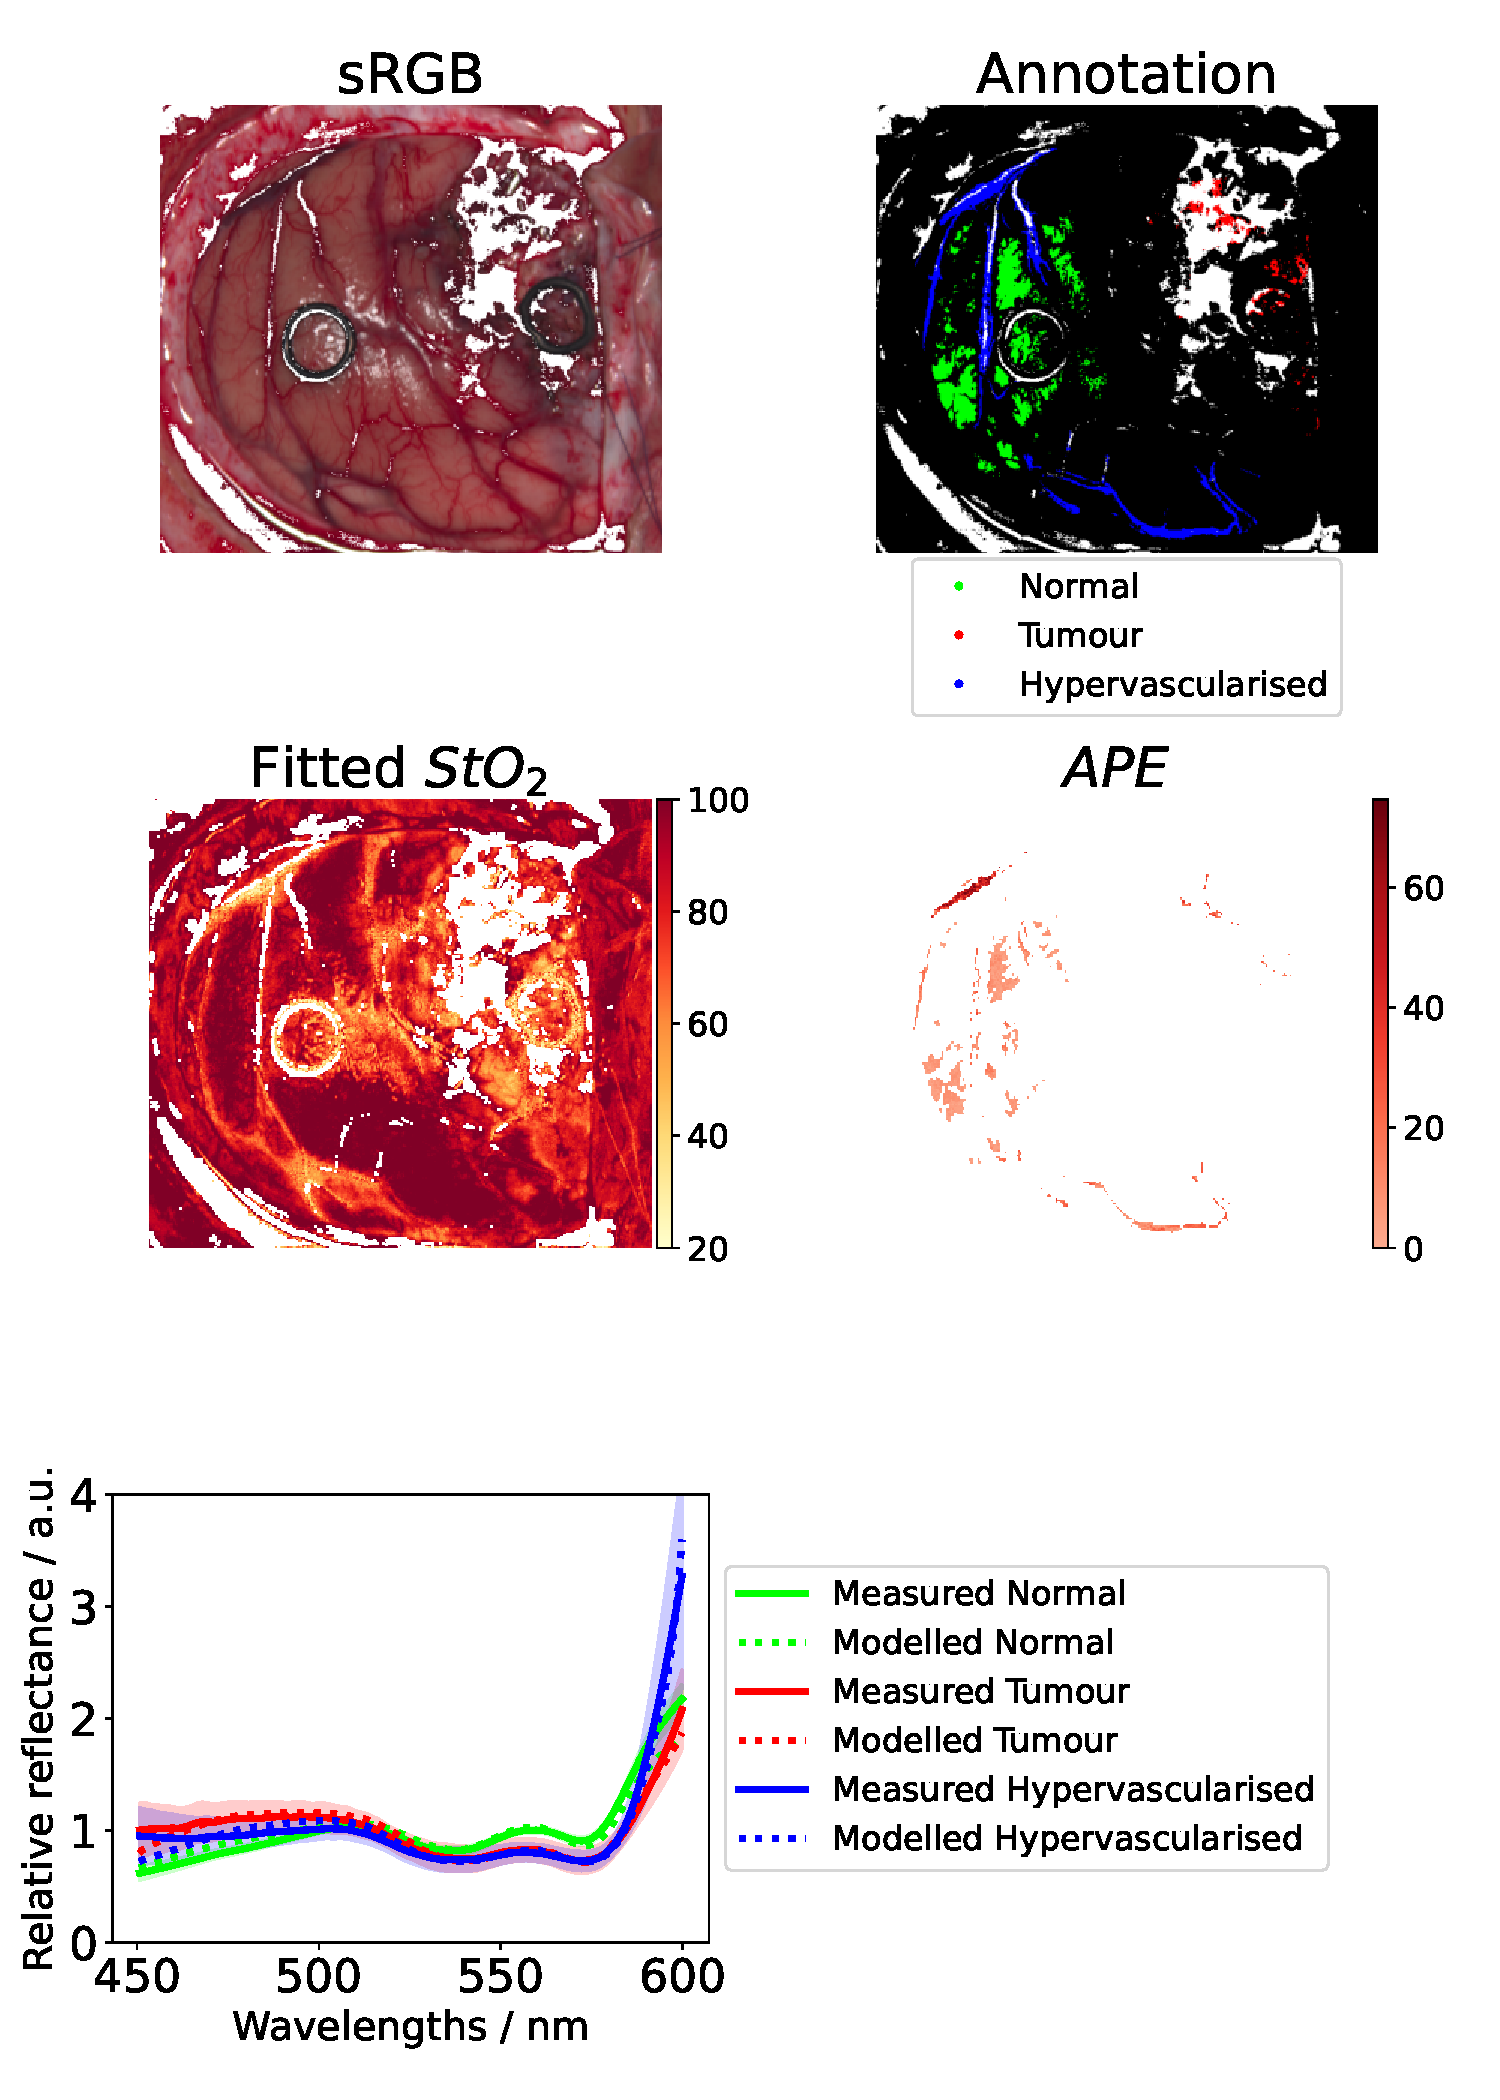
\includegraphics[width=\textwidth]{012-02_StO2_J.pdf}
    \caption{Top left shows an sRGB reconstruction of the HELICoiD image 012-02 with the regions beyond thresholds shown as white. Top right shows an annotation of the same image. Middle left shows the fitted $StO_2$ on a pixel-by-pixel basis using the Jacques 1999 single-layer model and method 4 (from \ref{sec:NeuroHSIdata}). Middle right shows the $APE$ of the fitted $StO_2$ of each pixel in each annotated region compared to the fitted $StO_2$ from the mean spectrum of the annotated region. Bottom shows the mean annotated spectra of each tissue type ($\pm$ standard deviation) plotted with the modelled spectra using parameters fitted to the mean annotated spectrum.}
    \label{ap:HELICoiDpixelJ}
\end{figure}
\FloatBarrier

\subsection{Using the mean of 5 frames}
\begin{figure}[h!]
    \centering 
    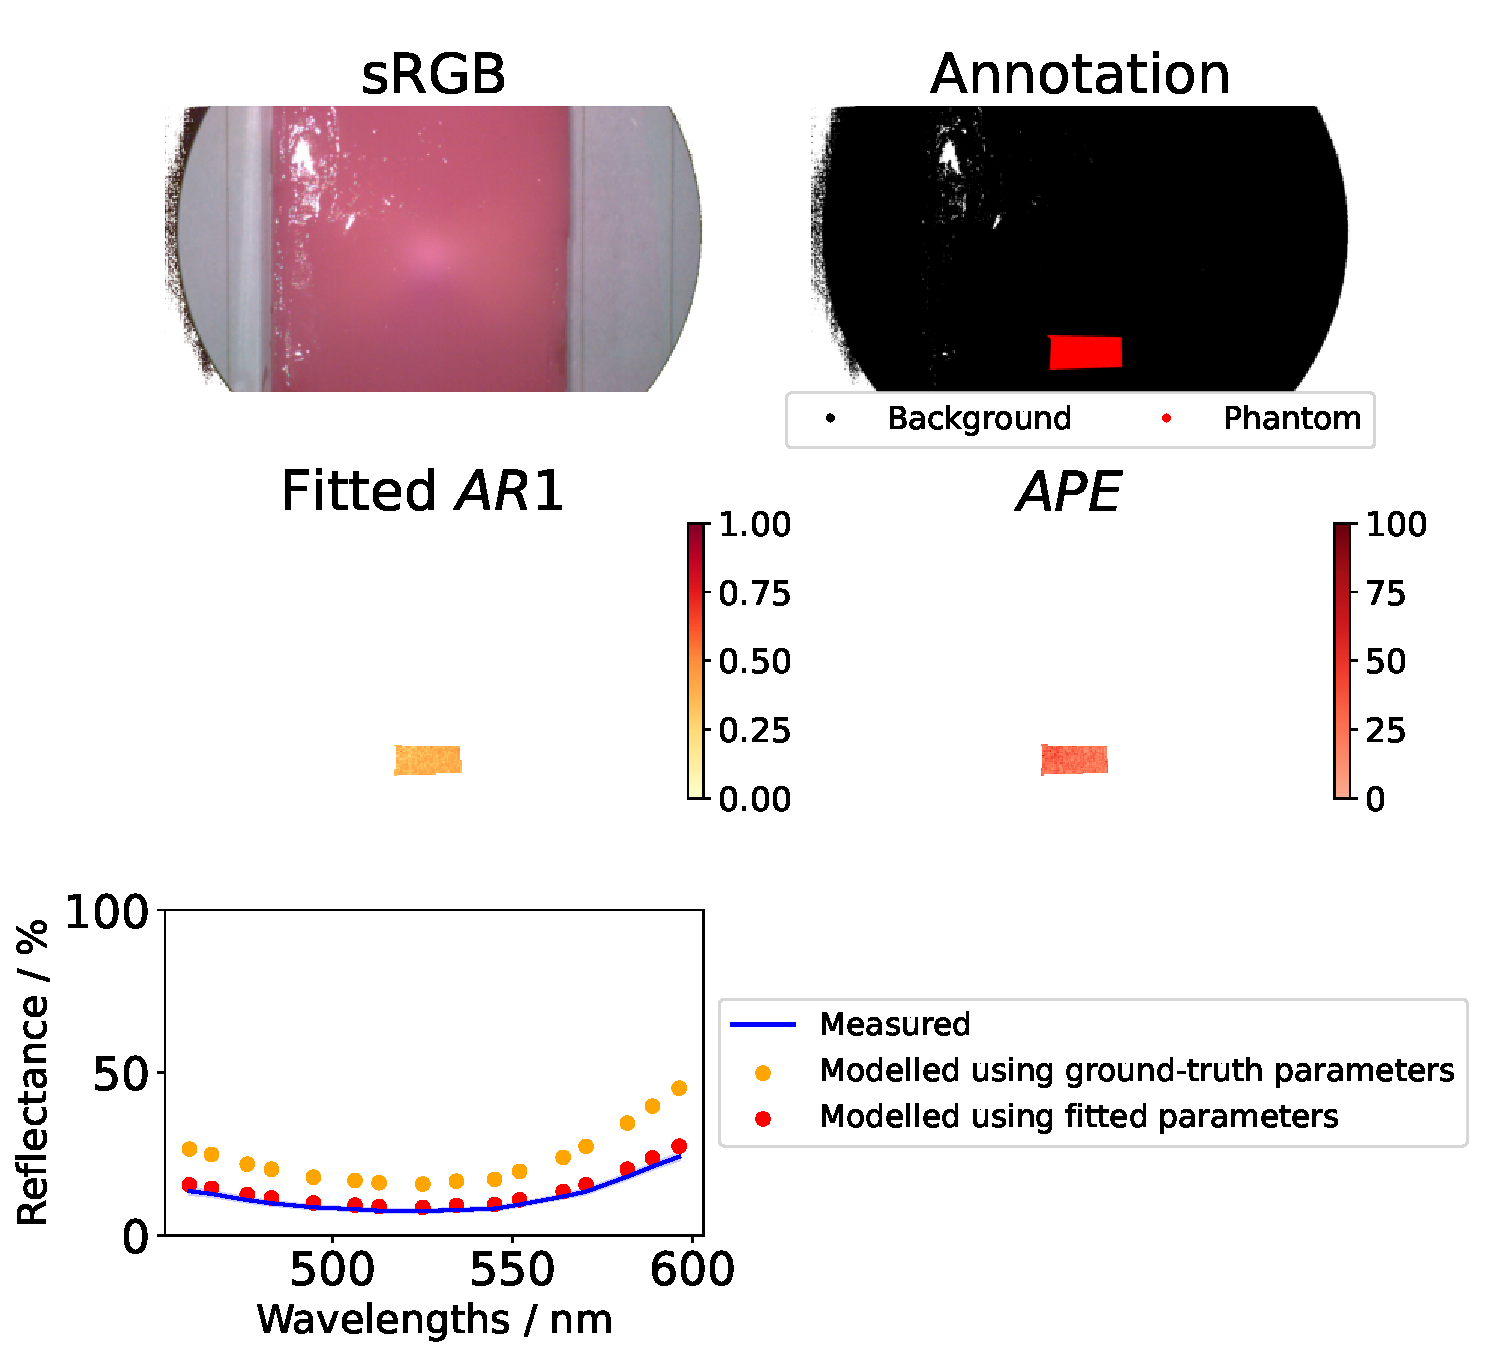
\includegraphics[width=\textwidth]{7_350_Y_OFF_AR1_5.pdf}
    \caption{Top left shows an sRGB reconstruction of the mean of 5 frames of a hyperspectral video of a gelatin-based phantom where $AR1=0.5$ and $I=3.50\%$ taken with a snapshot HSI camera, where the regions beyond thresholds are shown as white. Top right shows an annotation of the same image. Middle left shows the fitted $StO_2$ on a pixel-by-pixel basis of the quantitative data using the Yudovsky 2009 single-layer model. Middle right shows the $APE$ of the fitted $AR1$ of each pixel in the annotated region compared to the ground truth value (0.5). Bottom shows the mean annotated spectrum ($\pm$ standard deviation) plotted with the modelled spectrum using ground-truth parameters or parameters fitted to the mean annotated spectrum.}
    \label{ap:gelatinpbpegQY5}
\end{figure}

\begin{figure}[h!]
    \centering 
    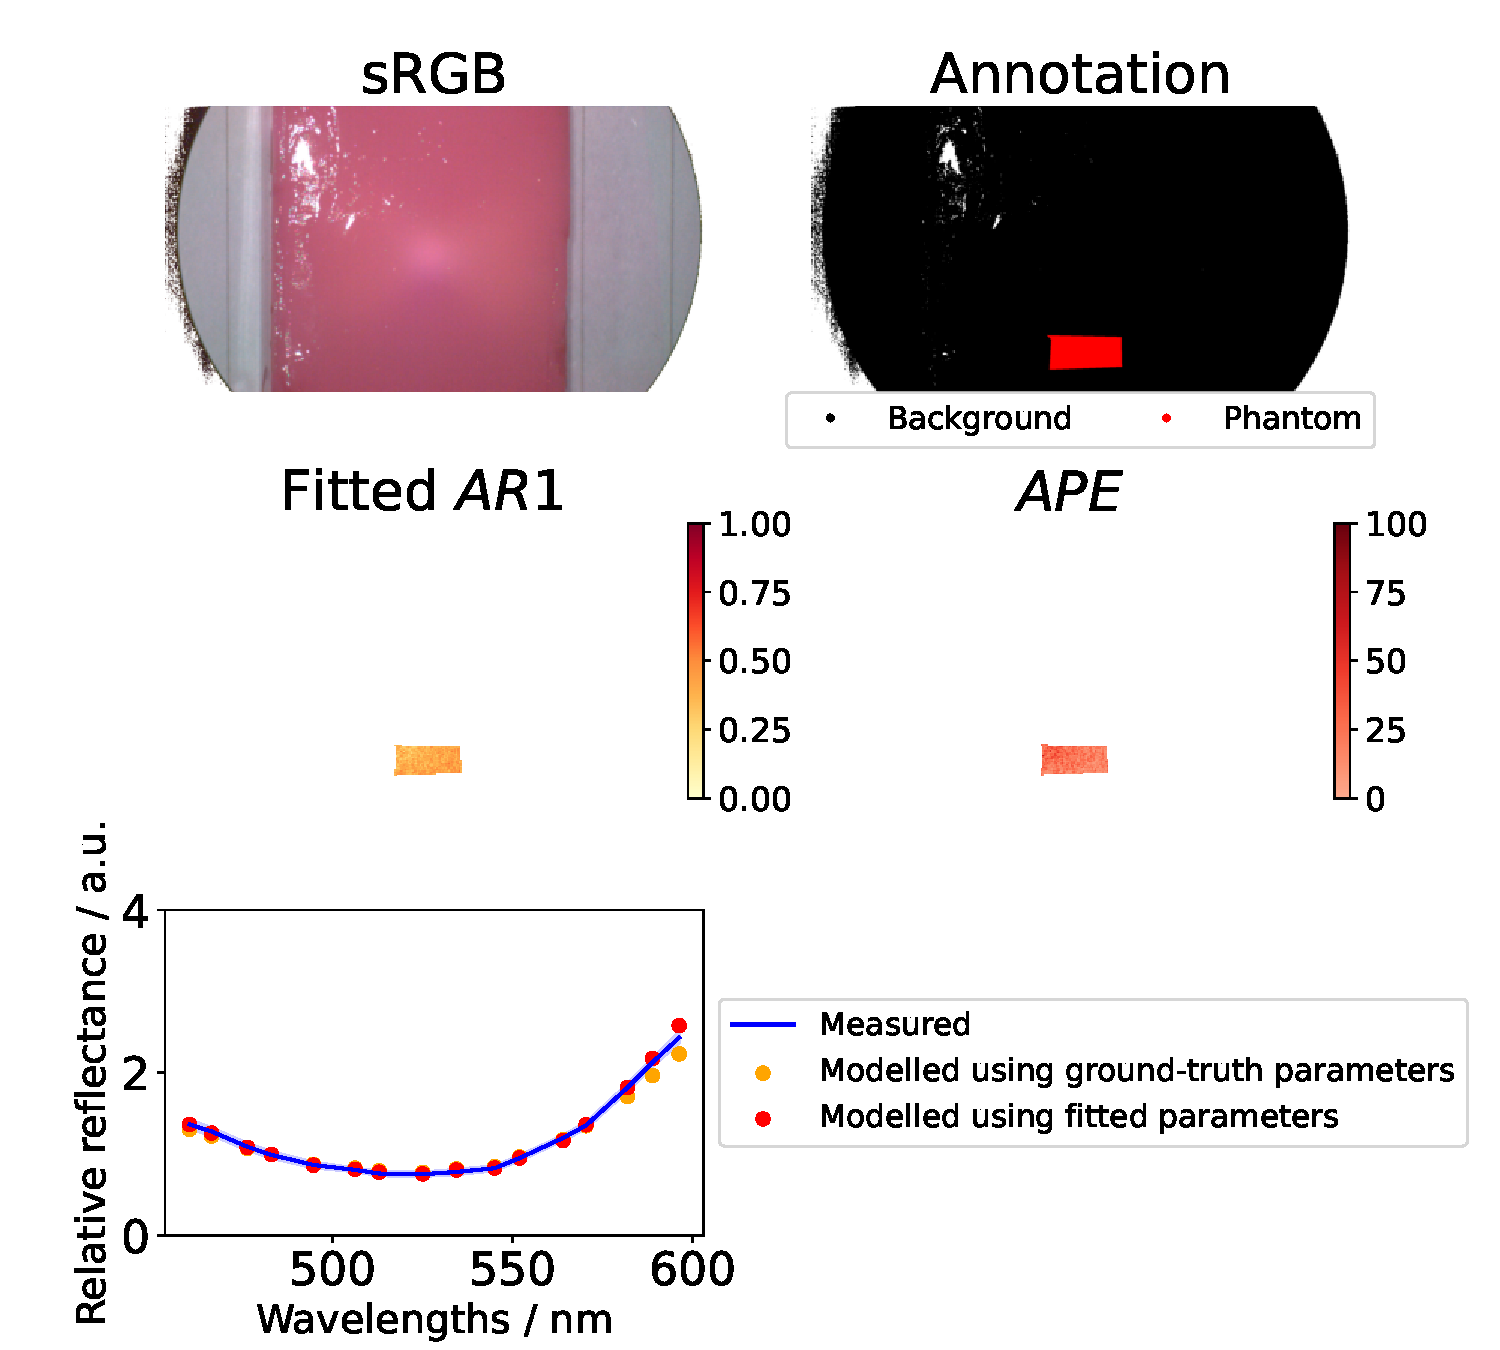
\includegraphics[width=\textwidth]{7_350_J_ON_AR1_5.pdf}
    \caption{Top left shows an sRGB reconstruction of the mean of 5 frames of a hyperspectral video of a gelatin-based phantom where $AR1=0.5$ and $I=3.50\%$ taken with a snapshot HSI camera, where the regions beyond thresholds are shown as white. Top right shows an annotation of the same image. Middle left shows the fitted $StO_2$ on a pixel-by-pixel basis of the relative data using the Jacques 1999 single-layer model. Middle right shows the $APE$ of the fitted $AR1$ of each pixel in the annotated region compared to the ground truth value (0.5). Bottom shows the mean annotated spectrum ($\pm$ standard deviation) plotted with the modelled spectrum using ground-truth parameters or parameters fitted to the mean annotated spectrum.}
    \label{ap:gelatinpbpegRJ5}
\end{figure}

\begin{figure}[h!]
    \centering 
    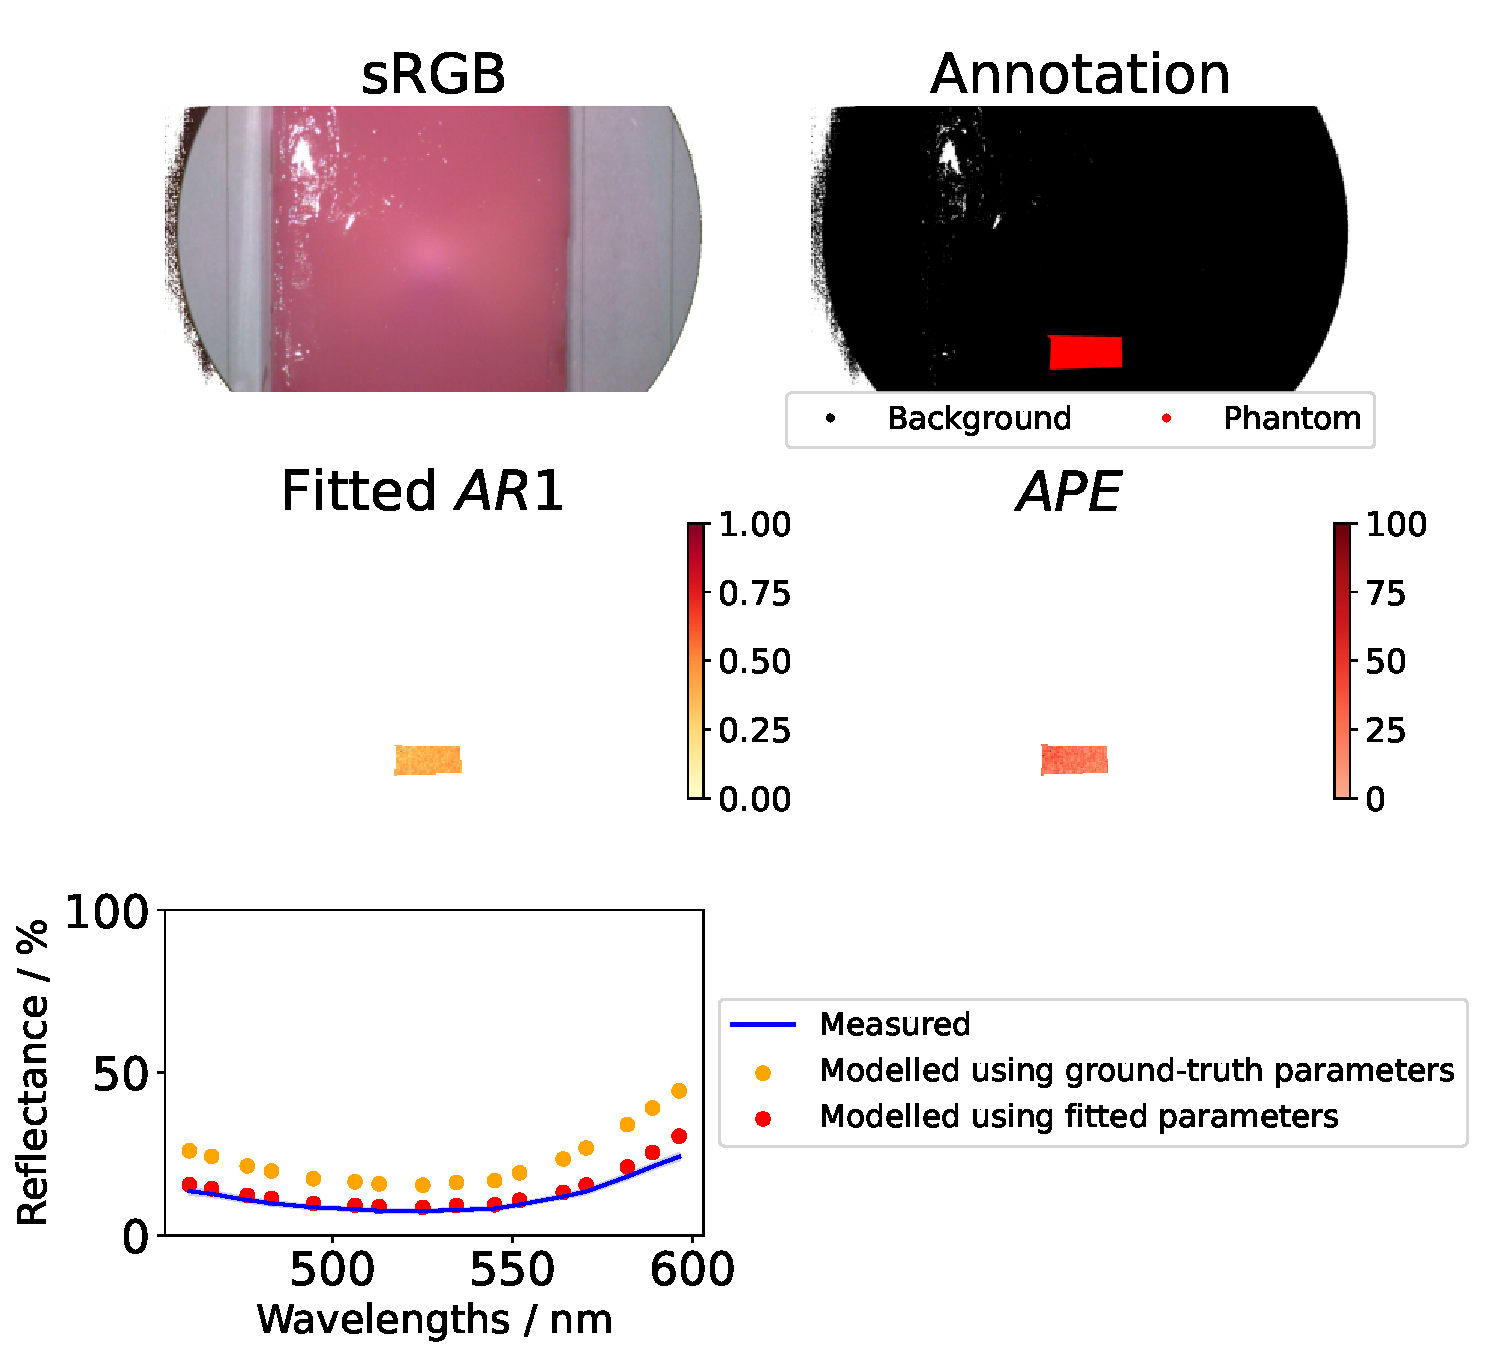
\includegraphics[width=\textwidth]{7_350_J_OFF_AR1_5.pdf}
    \caption{Top left shows an sRGB reconstruction of the mean of 5 frames of a hyperspectral video of a gelatin-based phantom where $AR1=0.5$ and $I=3.50\%$ taken with a snapshot HSI camera, where the regions beyond thresholds are shown as white. Top right shows an annotation of the same image. Middle left shows the fitted $StO_2$ on a pixel-by-pixel basis of the quantitative data using the Jacques 1999 single-layer model. Middle right shows the $APE$ of the fitted $AR1$ of each pixel in the annotated region compared to the ground truth value (0.5). Bottom shows the mean annotated spectrum ($\pm$ standard deviation) plotted with the modelled spectrum using ground-truth parameters or parameters fitted to the mean annotated spectrum.}
    \label{ap:gelatinpbpegQJ5}
\end{figure}
\FloatBarrier

\section{Appendices fitting Neurosurgical HSI data with uniform weighting of wavelengths}\label{ap:Chapter5uniform}
\begin{table}[h!]
    \centering
    \caption{The mean (standard deviation) of the fitted physiological parameters when extracted by fitting Yudovsky 2009 single layer (Y) or Jacques 1999 (J) to the relative mean annotated spectra for each tissue type of each image from the HELICoiD dataset using literature (L) or shifted (S) extinction coefficients with uniform weighting of the wavelengths and $n=1.44$. All presented to 3s.f.}
    \begin{tabular}{|ccc|cccc|}
        \hline
        \multirow{2}{*}{Tissue type} & \multirow{2}{*}{Model} & \multirow{2}{*}{Method} & $StO_2$ & $f_{blood}$ & $a$ & $b$ \\
        & & & (\%) & (\%) & ($cm^{-1}$) & (a.u.) \\
        \hline
        \multirow{4}{*}{\shortstack{Hyper-\\vascularised}} & \multirow{2}{*}{Y} & L & 84.0 (20.3) & 2.39 (2.08) & 48.9 (28.9) & 1.72 (1.24) \\
        & & S & 66.7 (27.5) & 3.67 (3.43) & 61.9 (14.8) & 1.50 (0.975) \\
        \cline{2-7}
        & \multirow{2}{*}{J} & L & 78.0 (20.8) & 6.64 (10.7) & 25.9 (27.2) & 1.76 (1.27) \\
        & & S & 55.2 (23.3) & 3.59 (4.42) & 16.0 (21.1) & 1.61 (1.05) \\
        \hline
        \multirow{4}{*}{Normal} & \multirow{2}{*}{Y} & L & 81.9 (22.7) & 0.782 (0.428) & 8.33 (1.85) & 0.318 (0.799) \\
        & & S & 78.0 (23.5) & 0.759 (0.388) & 8.32 (1.80) & 0.327 (0.800) \\
        \cline{2-7}
        & \multirow{2}{*}{J} & L & 84.0 (22.1) & 0.933 (0.701) & 8.46 (2.27) & 0.311 (0.798) \\
        & & S & 80.5 (23.2) & 0.855 (0.553) & 8.52 (2.27) & 0.323 (0.800) \\
        \hline
        \multirow{4}{*}{Tumour} & \multirow{2}{*}{Y} & L & 74.6 (23.6) & 1.06 (0.870) & 13.6 (18.7) & 0.282 (0.377) \\
        & & S & 78.0 (20.3) & 1.85 (2.01) & 26.3 (26.9) & 0.273 (0.324) \\
        \cline{2-7}
        & \multirow{2}{*}{J} & L & 73.9 (24.3) & 1.04 (0.655) & 8.00 (5.24$\times 10^{-15}$) & 0.205 (0.284) \\
        & & S & 75.7 (19.8) & 0.973 (0.545) & 9.94 (4.85) & 0.395 (0.368) \\
        \hline
    \end{tabular}    
    \label{tb:HELICoiDuniform}
\end{table}

\begin{figure}[h!]
    \centering
    \begin{subfigure}{0.49\textwidth}
        \includegraphics[width=\textwidth]{012-02Normal_spectra_Y_u.pdf}
        \caption{}
        \label{fig:backwardsHSIHeliYuniform}
    \end{subfigure}
    \begin{subfigure}{0.49\textwidth}
        \includegraphics[width=\textwidth]{012-02Normal_spectra_J_u.pdf}
        \caption{}
        \label{fig:backwardsHSIHeliJuniform}
    \end{subfigure}
    \begin{subfigure}{\textwidth}
        \includegraphics[width=\textwidth]{boxplotsHeli_u.pdf}
        \caption{}
        \label{fig:boxplotsHeliuniform}
    \end{subfigure}
    \caption{An example of the visual fitting quality of the Yudovsky 2009 (\ref{fig:backwardsHSIHeliY}) and Jacques 1999 (\ref{fig:backwardsHSIHeliJ}) single layer models when fitting to the relative mean annotated spectrum ($\pm$1 standard deviation, \textcolor{blue}{blue solid}) of the normal tissue class of HELICoiD image 12-02 using literature (L) or shifted (S) extinction coefficients and a uniform wavelength weighting. The distribution of the fitted physiological parameters retrieved by fitting each model to each relative mean annotated spectrum of the tissue classes of each HELICoiD image is shown in \ref{fig:boxplotsHeli}.}
    \label{fig:HELICoiDannuniform}
\end{figure}
\FloatBarrier
\end{subappendices}